% beamer 16:9
\documentclass[aspectratio=169, 9pt, xcolor=dvipsnames]{beamer}
\usecolortheme[named=NavyBlue]{structure}
\beamertemplatenavigationsymbolsempty
\setbeamertemplate{footline}[frame number]
\usefonttheme{serif}
\setbeamertemplate{caption}[numbered]
\setbeamerfont*{itemize/enumerate subbody}{parent=itemize/enumerate body}
% math package
\usepackage{amsmath, amsthm, amssymb, booktabs, multirow, hyperref, pgffor, tabularx, makecell}
\usepackage{kotex}
\usepackage[backend=biber,style=authoryear]{biblatex}

\title{Parameter estimation of age-structured model for SARS-CoV-2 in Seoul and Gyeonggi}
\author{Yunjeong Lee, Jeongjoo Seok}
\institute{School of Mathematics and Computing\\
(Computational Science and Engineering)\\
Yonsei University}
\date{\today}

\addbibresource{210909_ref.bib}

\begin{document}
	
	\begin{frame}\frametitle{}
	    \maketitle
	\end{frame}

	\begin{frame}\frametitle{Data}
	    \begin{enumerate}
	    	\item Daily confirmed cases in Seoul and Gyeonggi
	    	\item Vaccine
	    	\begin{itemize}
	    		\item Daily number of vaccination for 1st dose (by age)
	    		\item Daily number of vaccination for 2nd dose (by age)
	    		\item Vaccine efficacy
	    	\end{itemize}
	    	\item Proportion of $\delta$ variant
	   	\end{enumerate}
	\end{frame}

	\begin{frame}\frametitle{Data processing}
	    \textbf{1. Daily number of vaccination for 1st dose (all ages)}
	    \begin{figure}
	    	\centering
	    	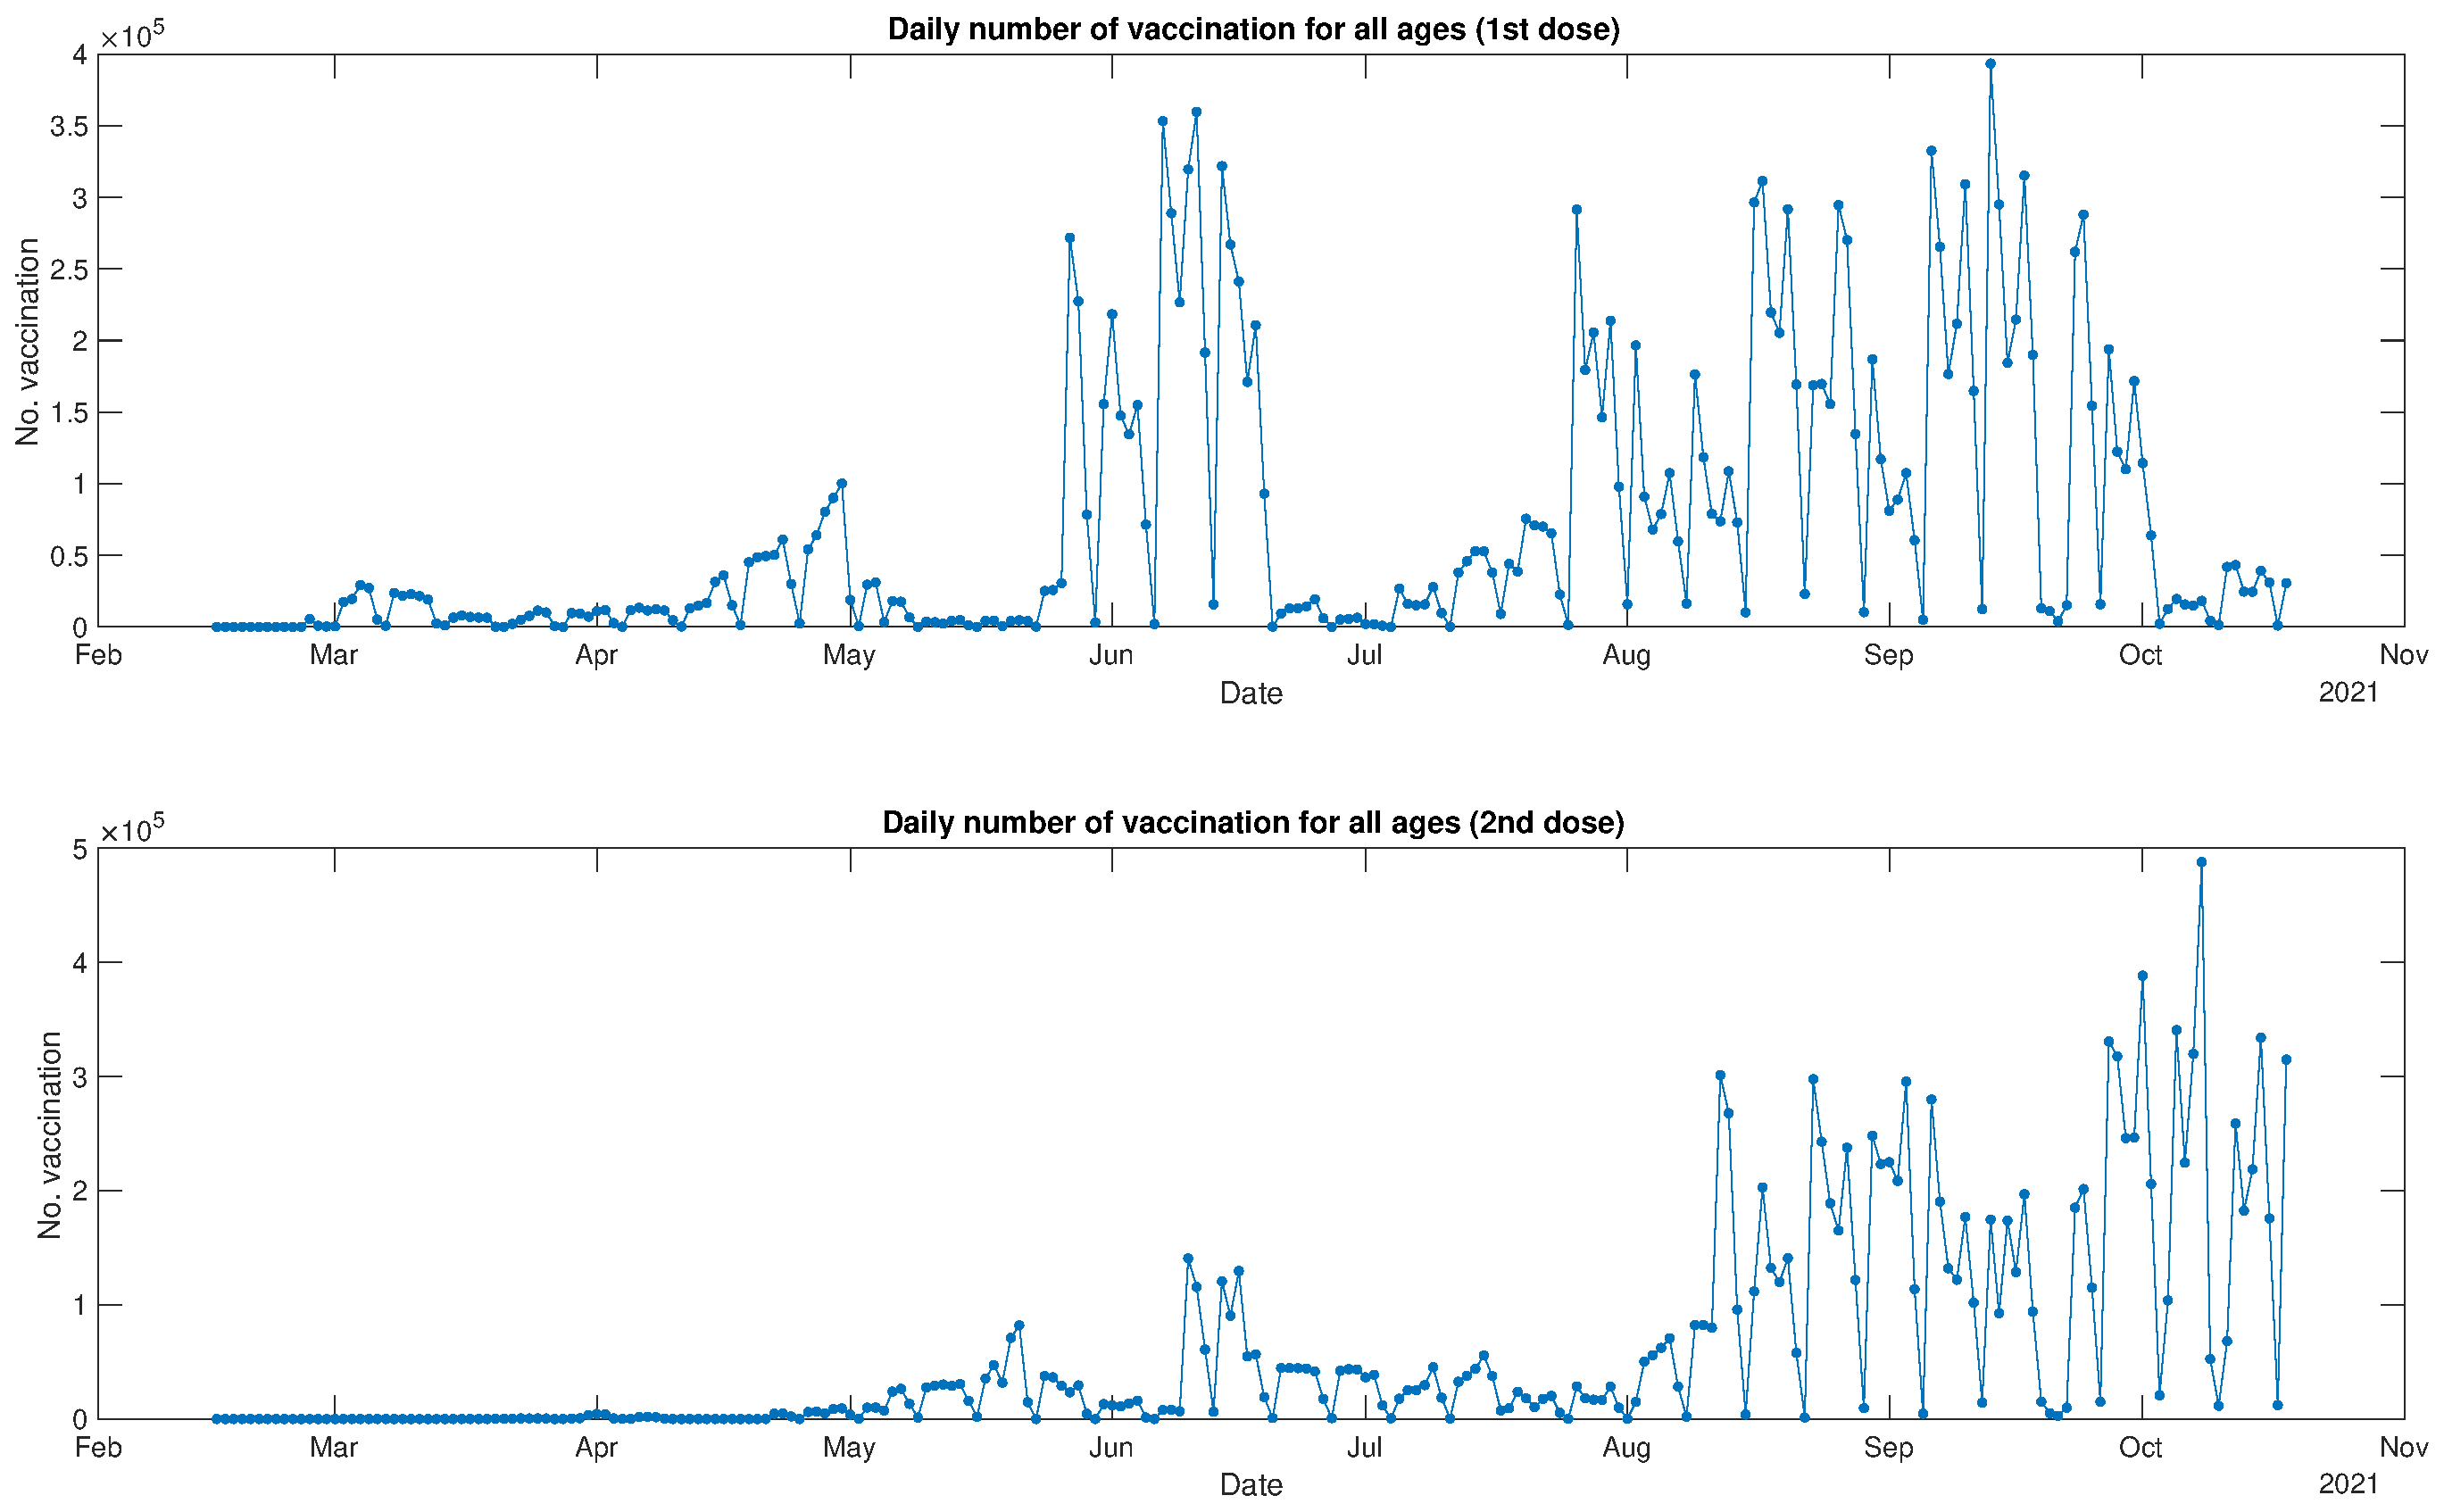
\includegraphics[width=10cm]{../results/data/vaccine_number.eps}
	    	\caption{The daily number vaccination for 1st dose and 2nd dose from 2021/02/15 to 2021/09/01}
	    \end{figure}
	\end{frame}

	\begin{frame}\frametitle{Data processing}
	    \textbf{1. Daily number of vaccination for 1st dose (by age)}
	    \begin{itemize}
	    	\item The daily number of vaccination by age is generated by the ratio between ages of vaccinated people.
	    	\item The ratio is based on KDCA reports.
	    \end{itemize}
	    \begin{figure}
	    	\centering
	    	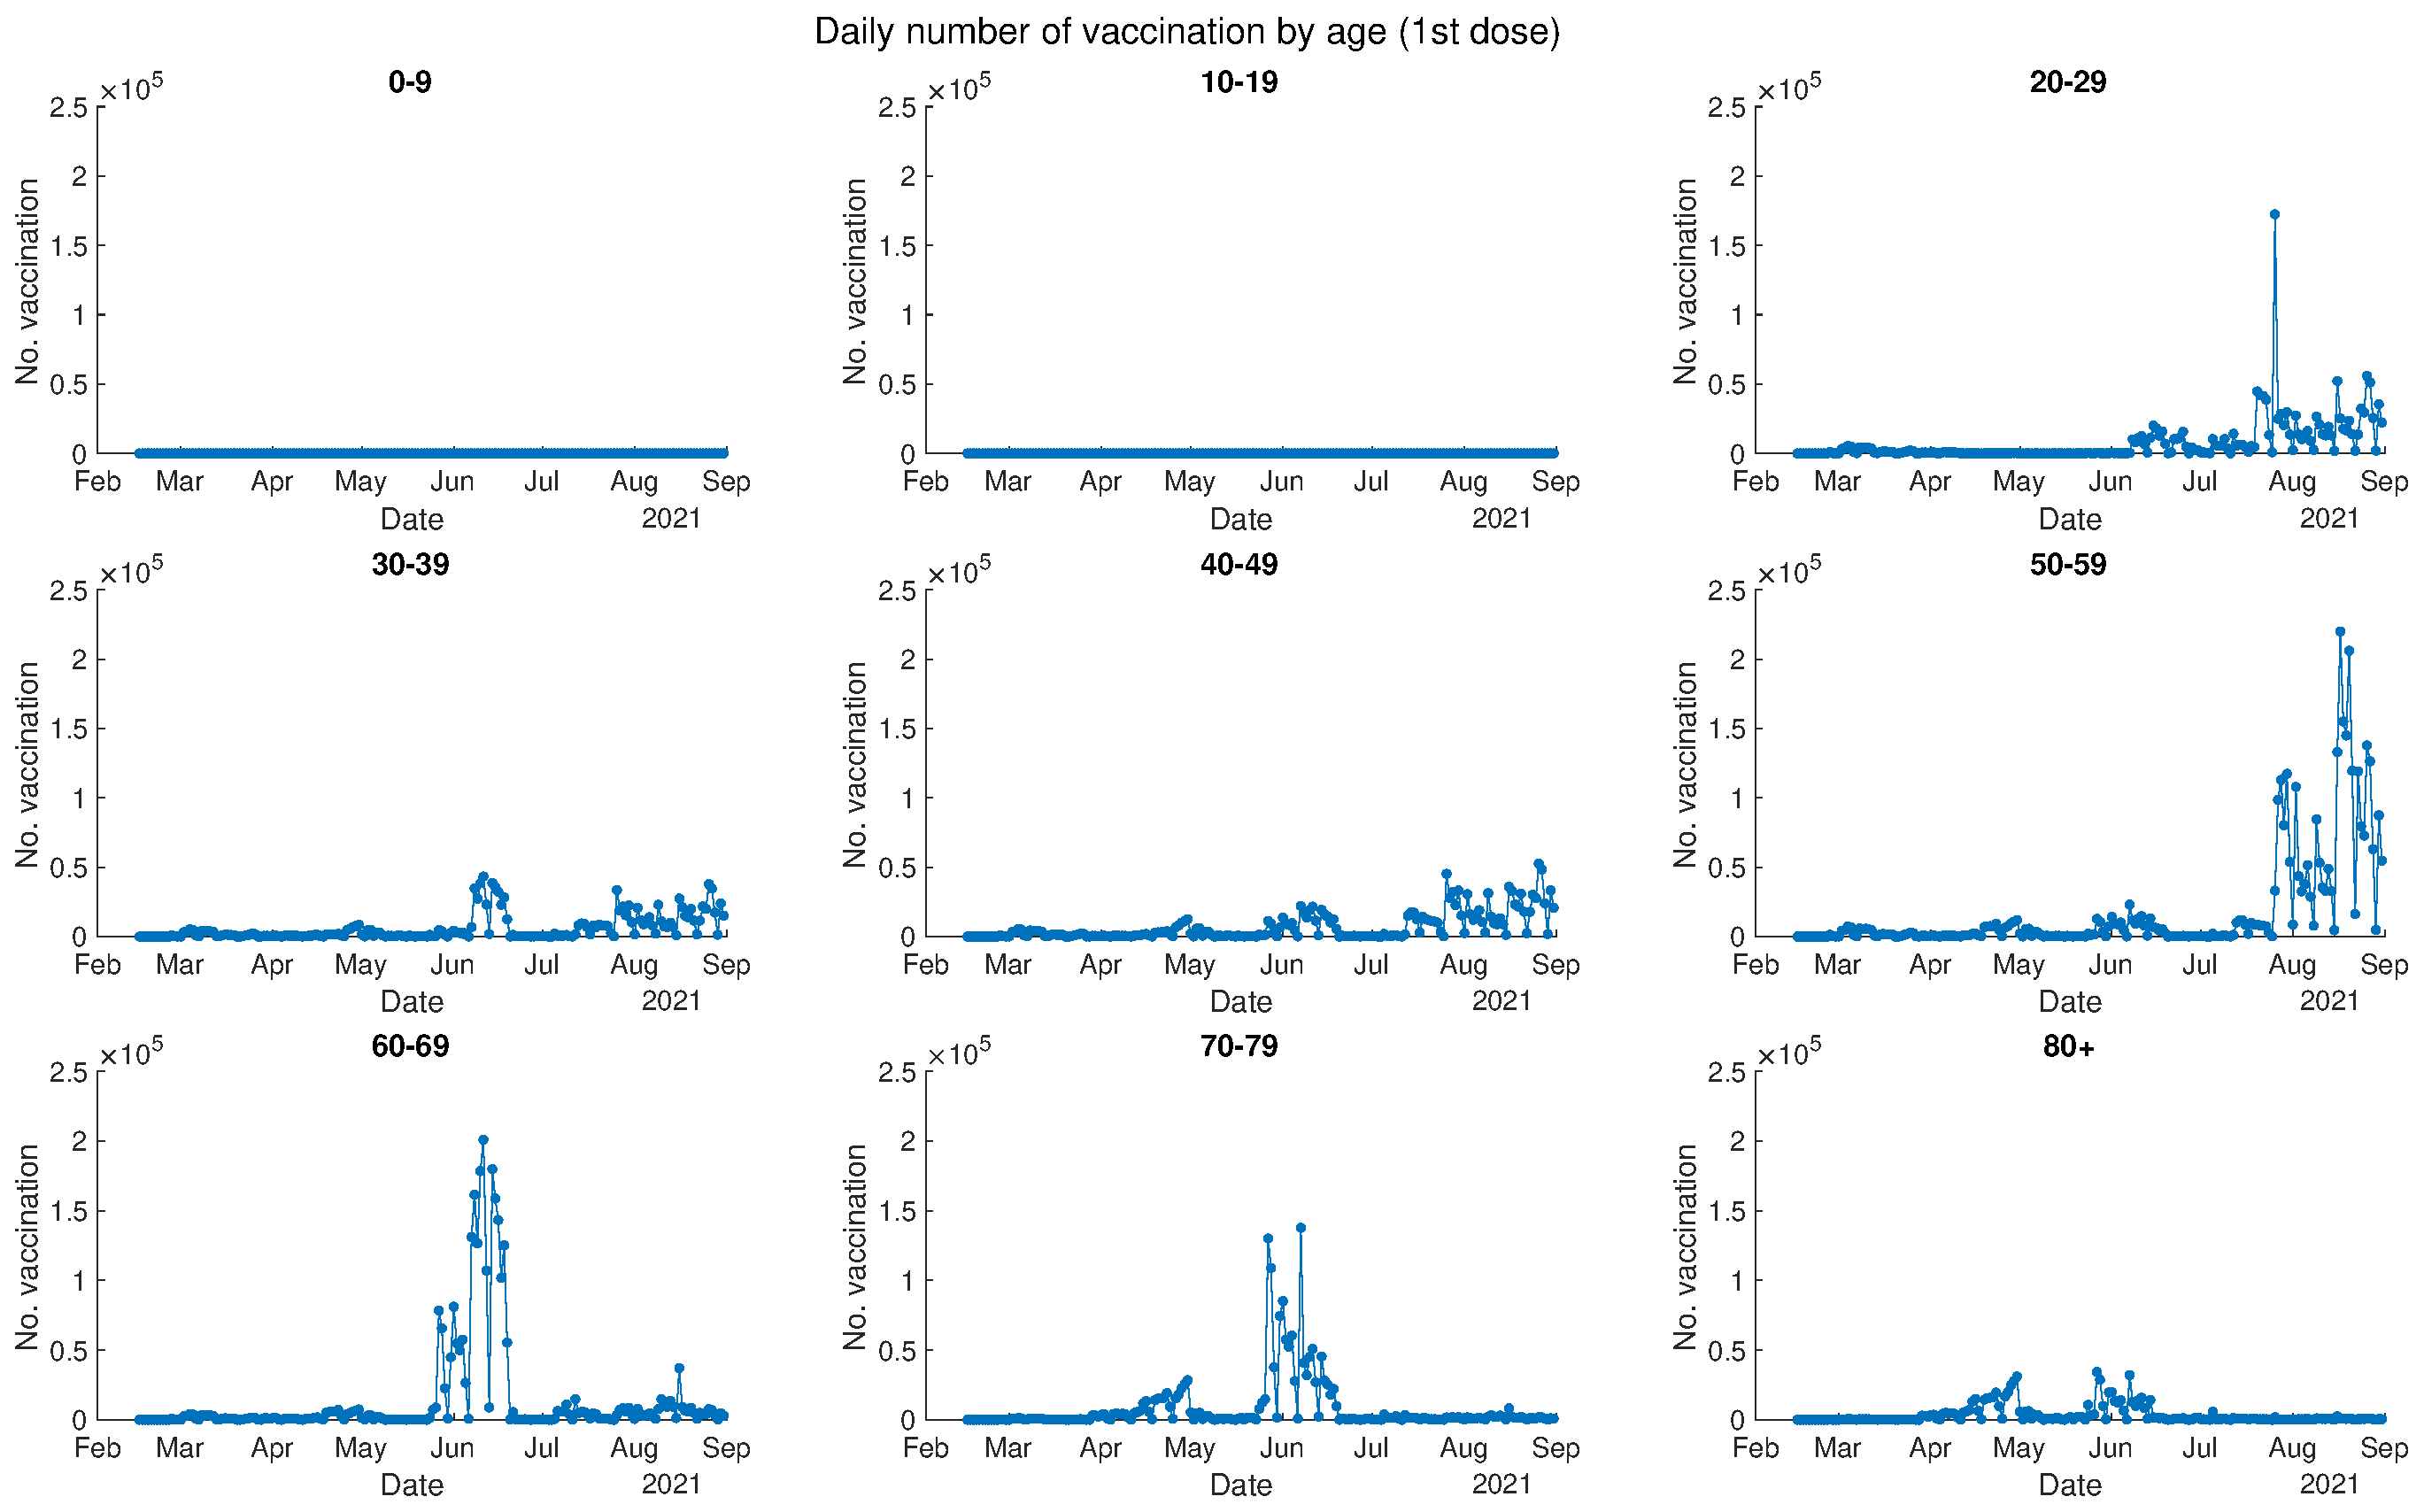
\includegraphics[width=8cm]{../results/data/vaccine_number_by_age_1st.eps}
	    	\caption{The daily number vaccination for 1st dose by age from 2021/02/15 to 2021/09/01}
	    \end{figure}
	\end{frame}

	\begin{frame}\frametitle{Data processing}
	    \textbf{2. Daily number of vaccination for 2nd dose (by age)}
	    \begin{itemize}
	    	\item The daily number of vaccination by age is generated by the ratio between ages of vaccinated people.
	    	\item The ratio is based on KDCA reports.
	    \end{itemize}
	    \begin{figure}
	    	\centering
	    	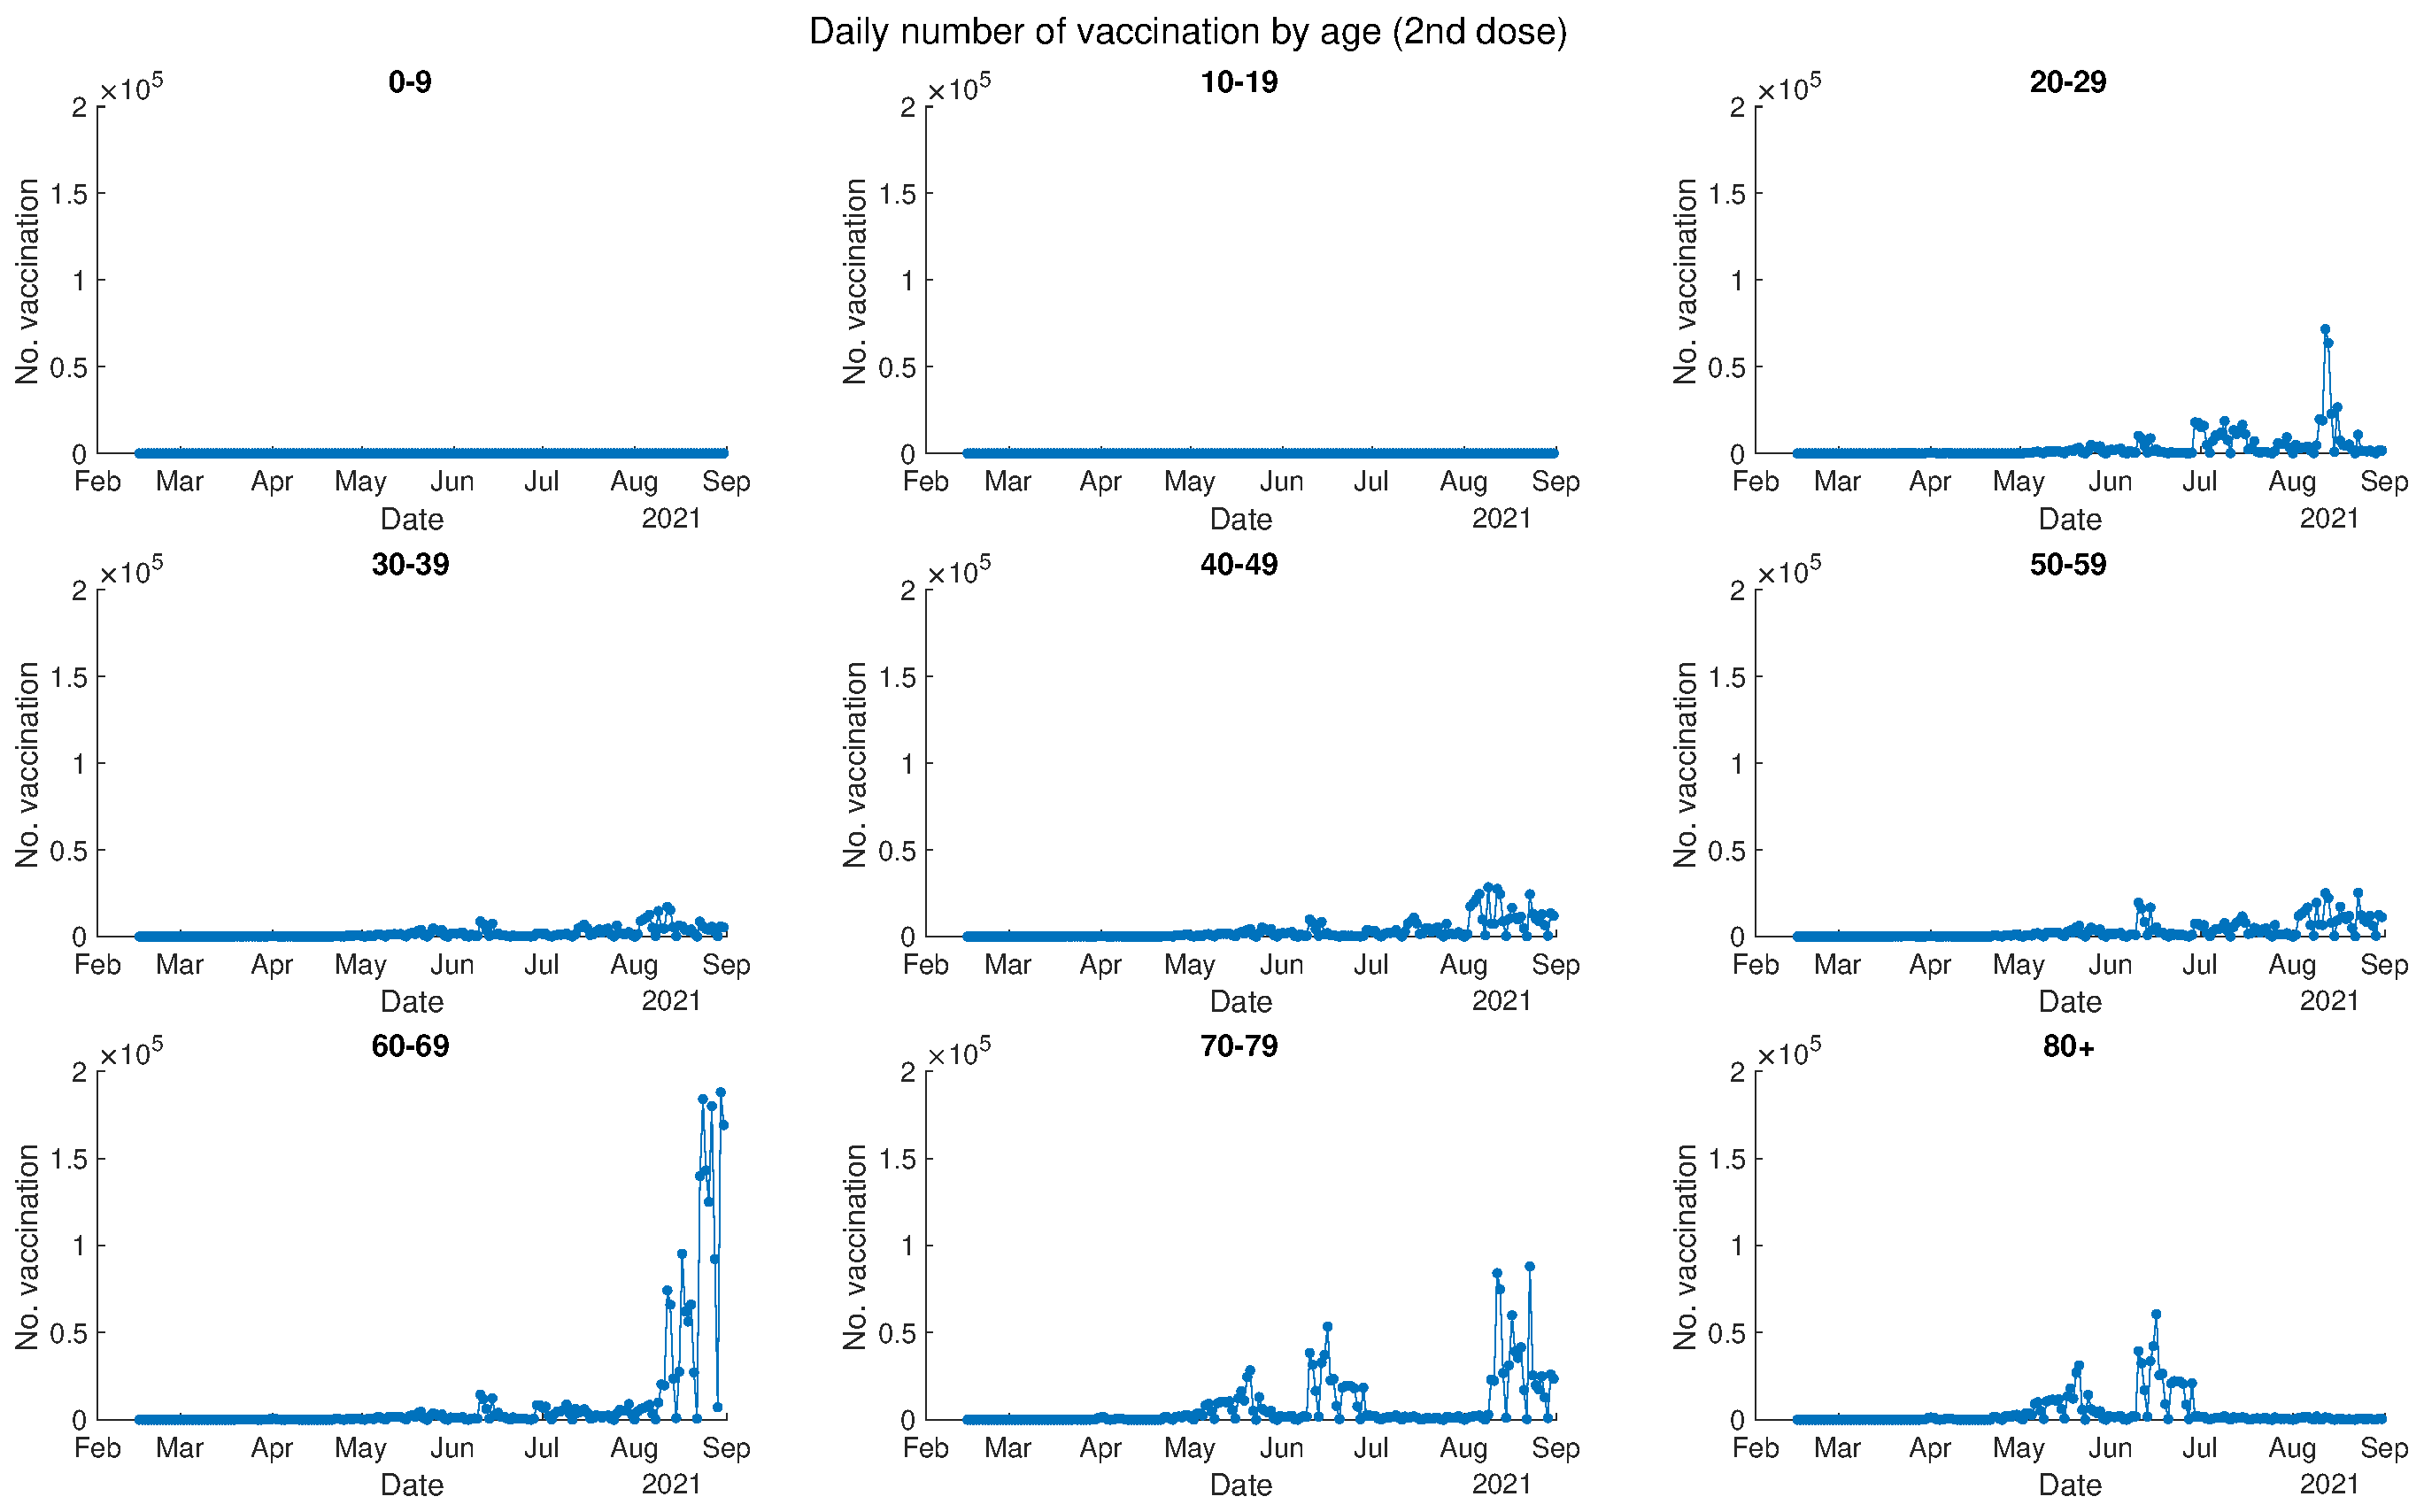
\includegraphics[width=8cm]{../results/data/vaccine_number_by_age_2nd.eps}
	    	\caption{The daily number vaccination for 2nd dose by age from 2021/02/15 to 2021/09/01}
	    \end{figure}
	\end{frame}

	\begin{frame}\frametitle{Data processing}
	    \textbf{3. Vaccine efficacy}
		\begin{itemize}
			\item The vaccine efficacies for $\alpha$ variant and $\delta$ variant are different.\footnotemark[1]
			\item We use weighted sum of vaccine efficacies where weights are based on proportion of $\delta$ variant
		\end{itemize}
		\begin{table}
			\begin{tabular}{c|crr}
				\toprule
				& \textbf{Astrazeneca} & \textbf{Pfizer} \\
				\midrule
				\multirow{2}{*}{$\mathbf{\alpha}$ variant} & \textbf{1st dose} & 48.7\% & 47.5\% \\
				& \textbf{2nd dose} & 74.5\% & 93.7\% \\
				\midrule
				\multirow{2}{*}{$\mathbf{\delta}$ variant} & \textbf{1st dose} & 30.0\% & 35.6\% \\
				& \textbf{2nd dose} & 67\% & 88\% \\
				\bottomrule
			\end{tabular}
		\end{table}
		\footnotetext[1]{\fullcite{bernal2021effectiveness}}
	\end{frame}

	\begin{frame}\frametitle{Data processing}
	    \textbf{3. Vaccine efficacy}
		\begin{figure}
			\centering
			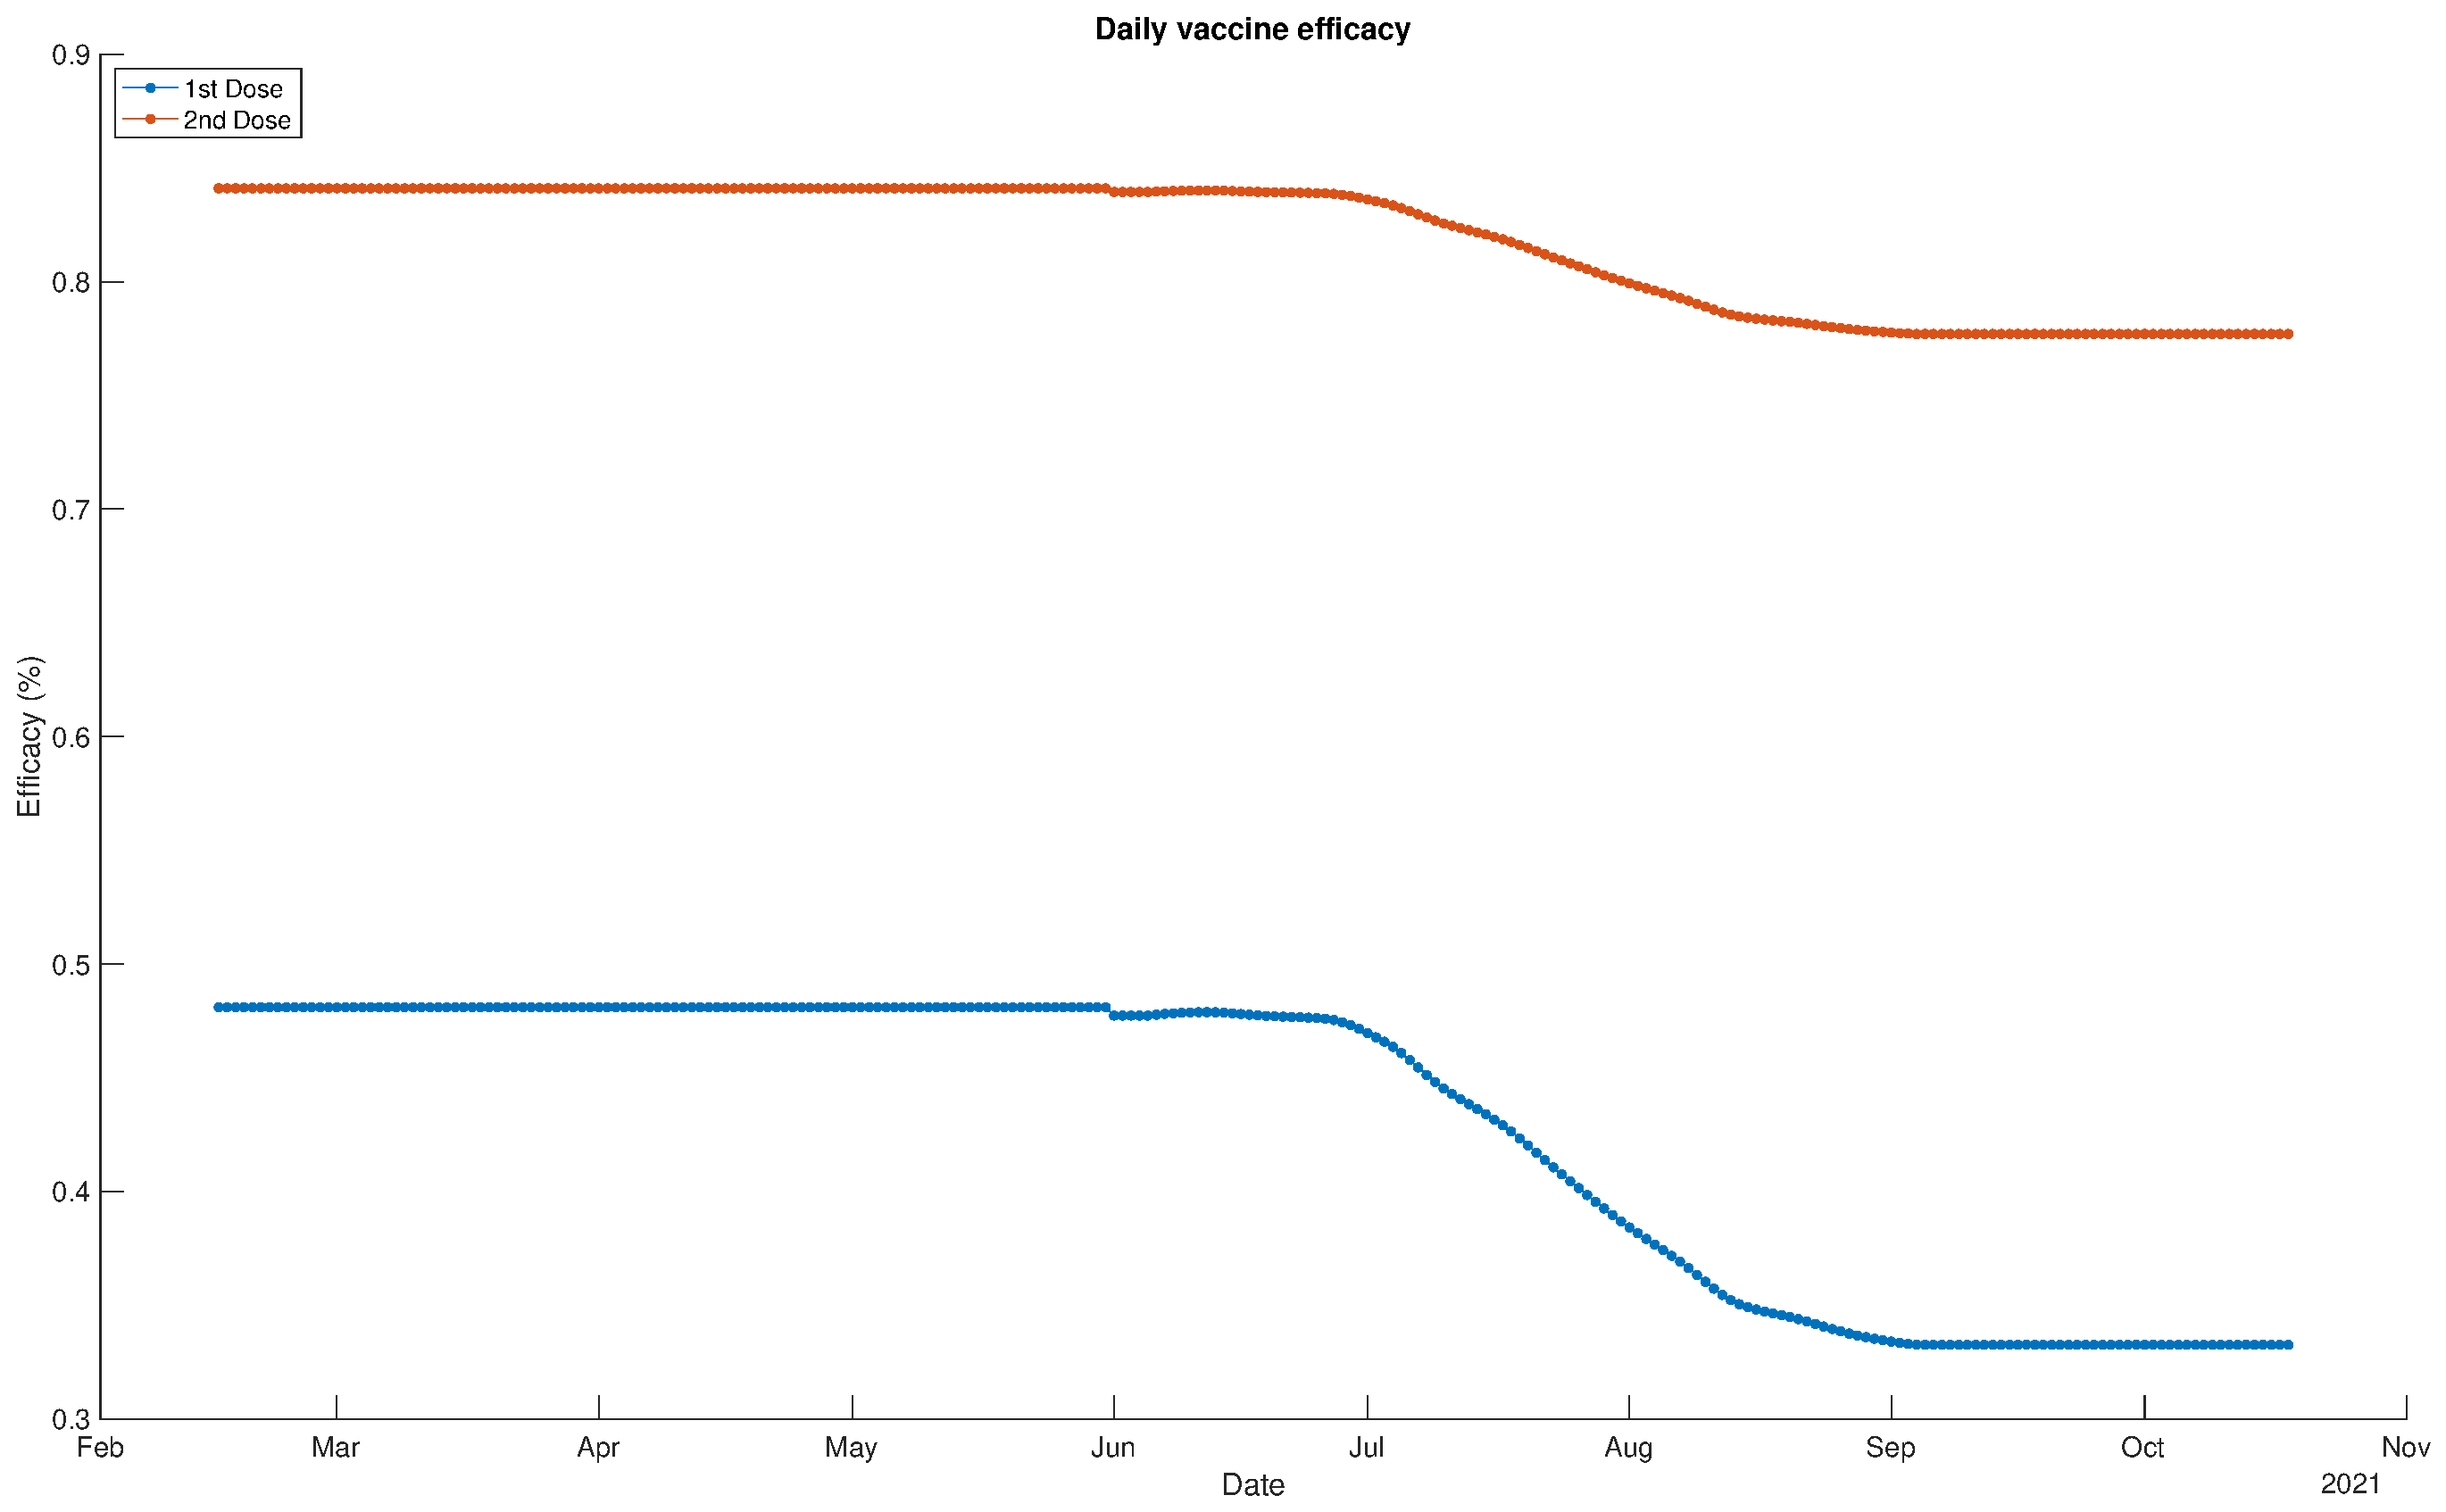
\includegraphics[width=10cm]{../results/data/vaccine_efficacy.eps}
			\caption{The estimated daily vaccine efficacy for 1st dose and 2nd dose.}
		\end{figure}
	\end{frame}

	\begin{frame}\frametitle{Data processing}
	    \textbf{4. Proportion of $\delta$ variant} \\
	    \begin{minipage}{0.3\textwidth}
	    	\begin{figure}
		    	\centering
		    	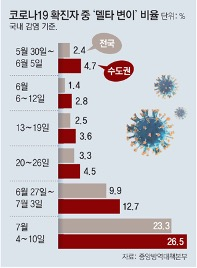
\includegraphics[width=\textwidth]{delta.jpg}
		    \end{figure}
	    \end{minipage}
	    \hfill
	    \begin{minipage}{0.6\textwidth}
	    	\begin{figure}
	    		\centering
	    		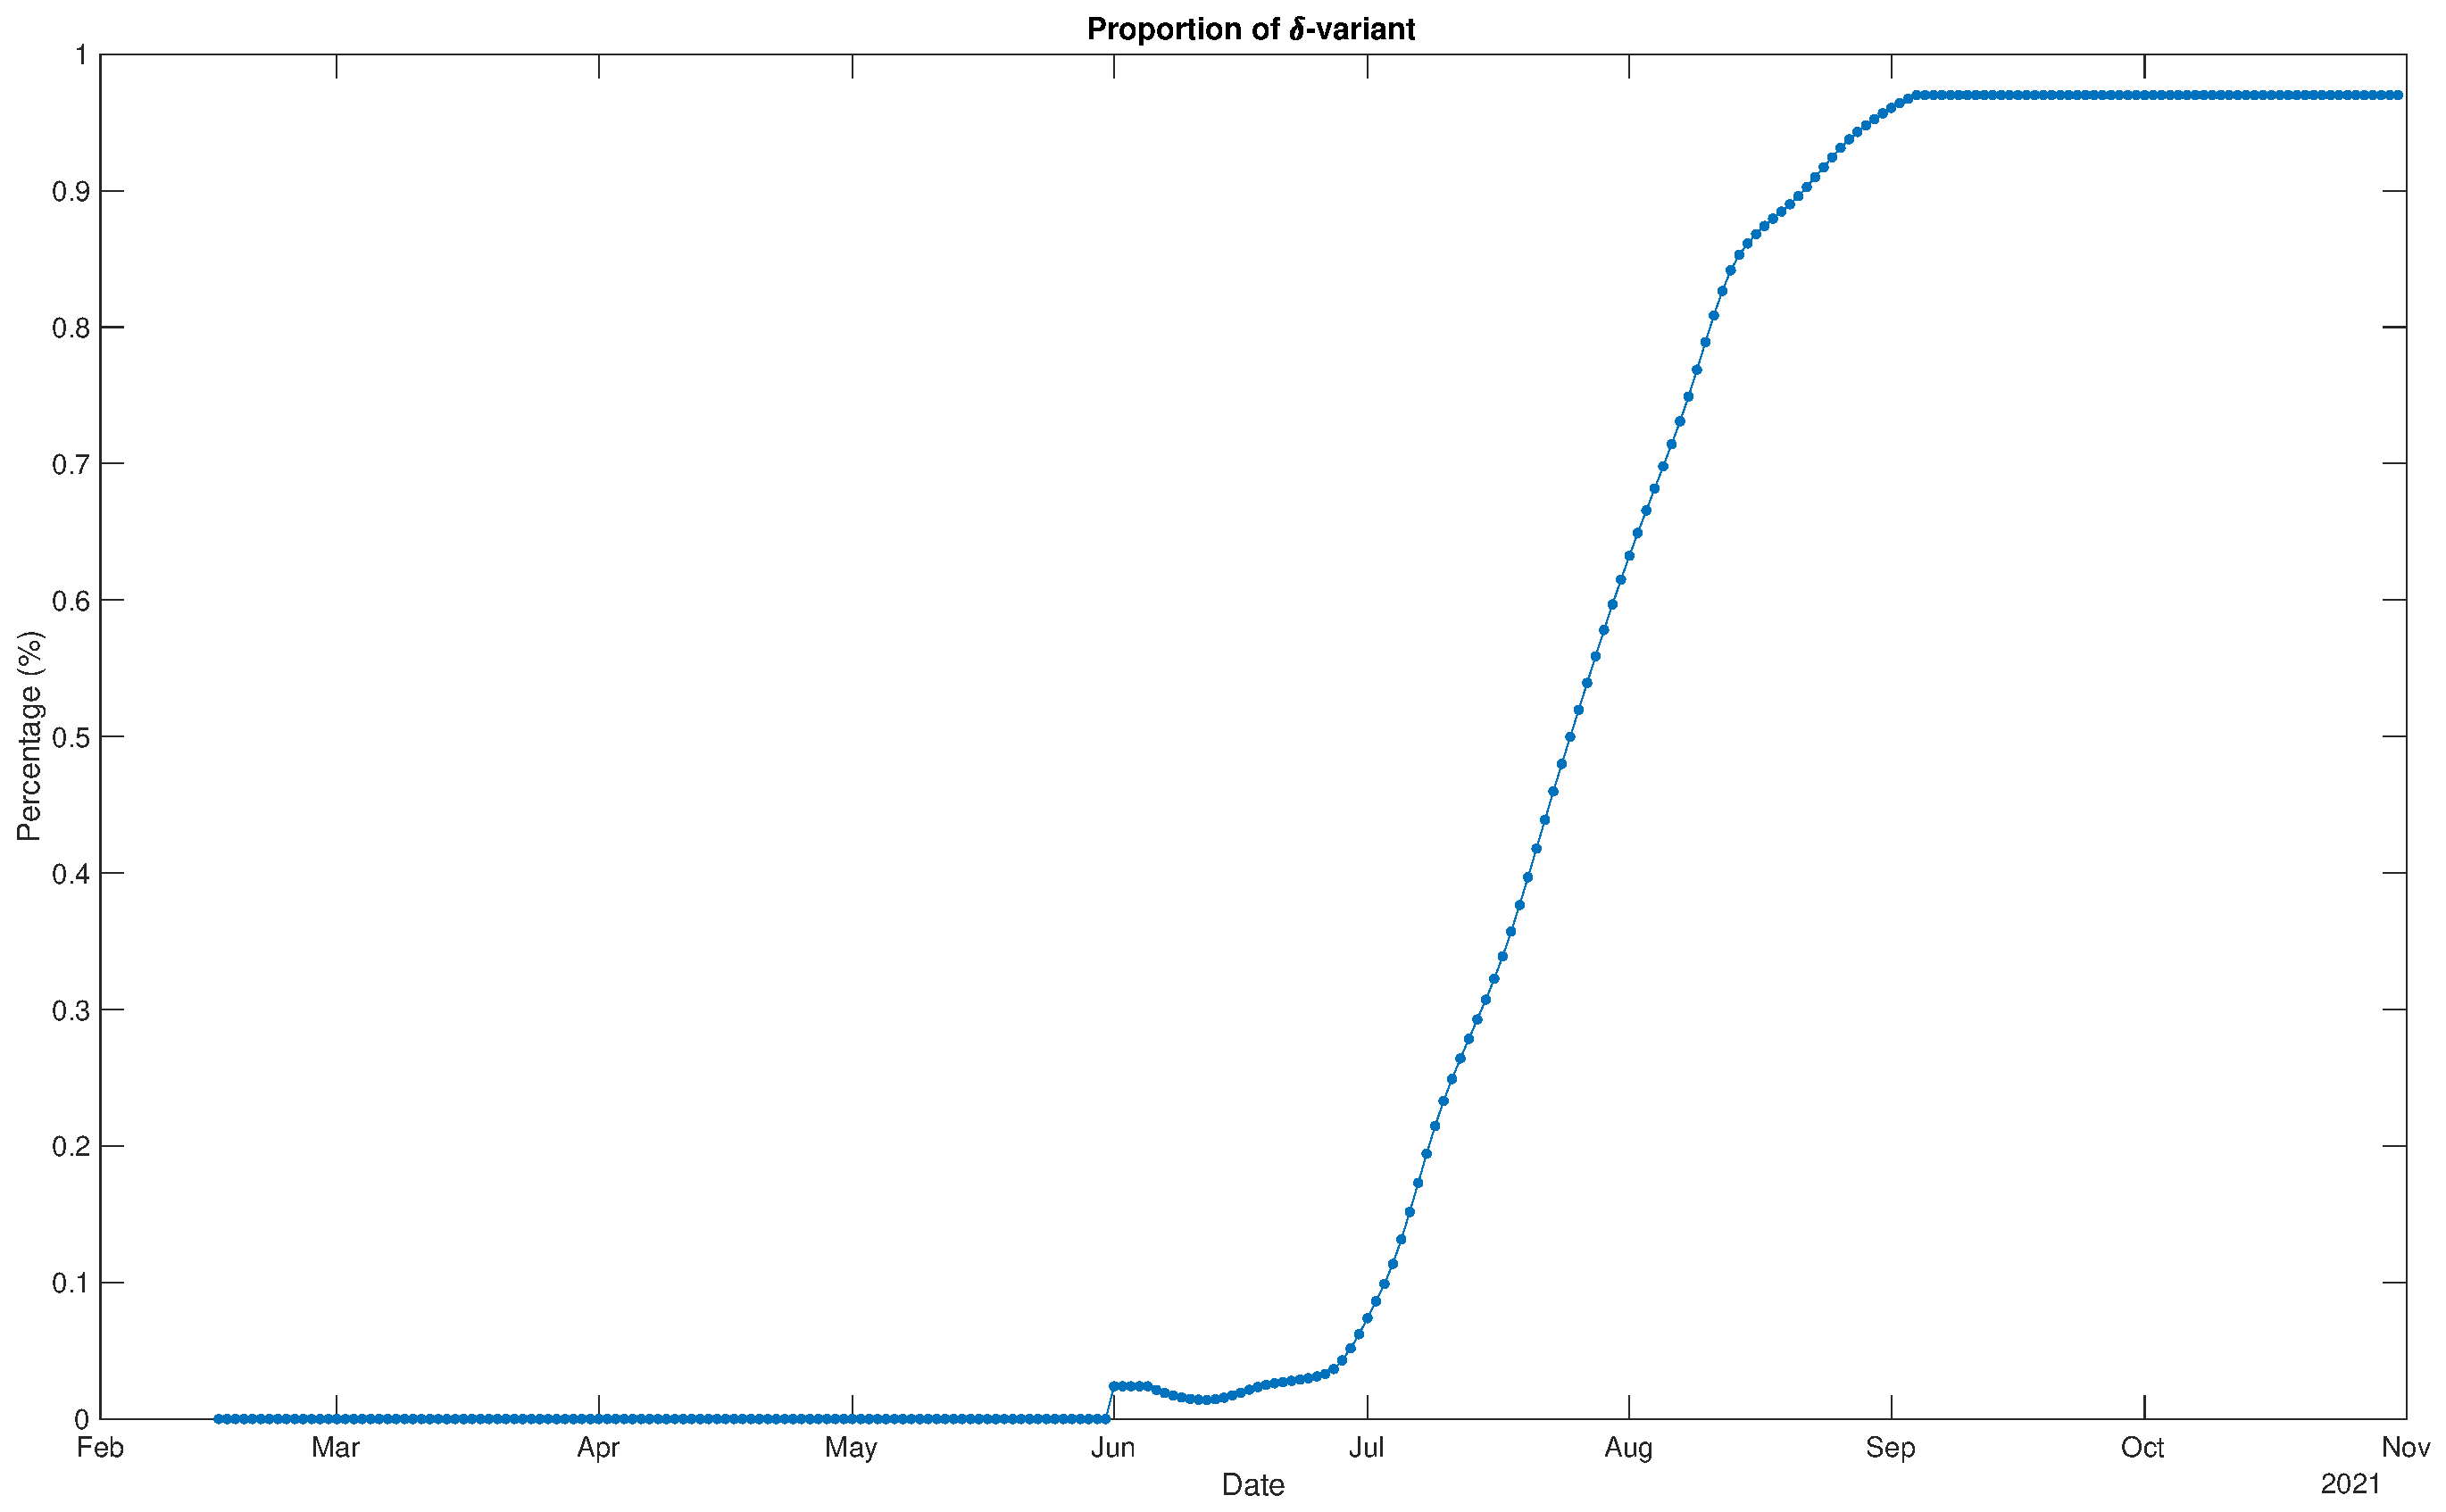
\includegraphics[width=\textwidth]{../results/data/delta_proportion.eps}
	    		\caption{Estimates of proportion of $\delta$ variant.}
	    	\end{figure}
	    \end{minipage}
	\end{frame}

	\begin{frame}\frametitle{Model}
	    \begin{figure}
	    	\centering
	    	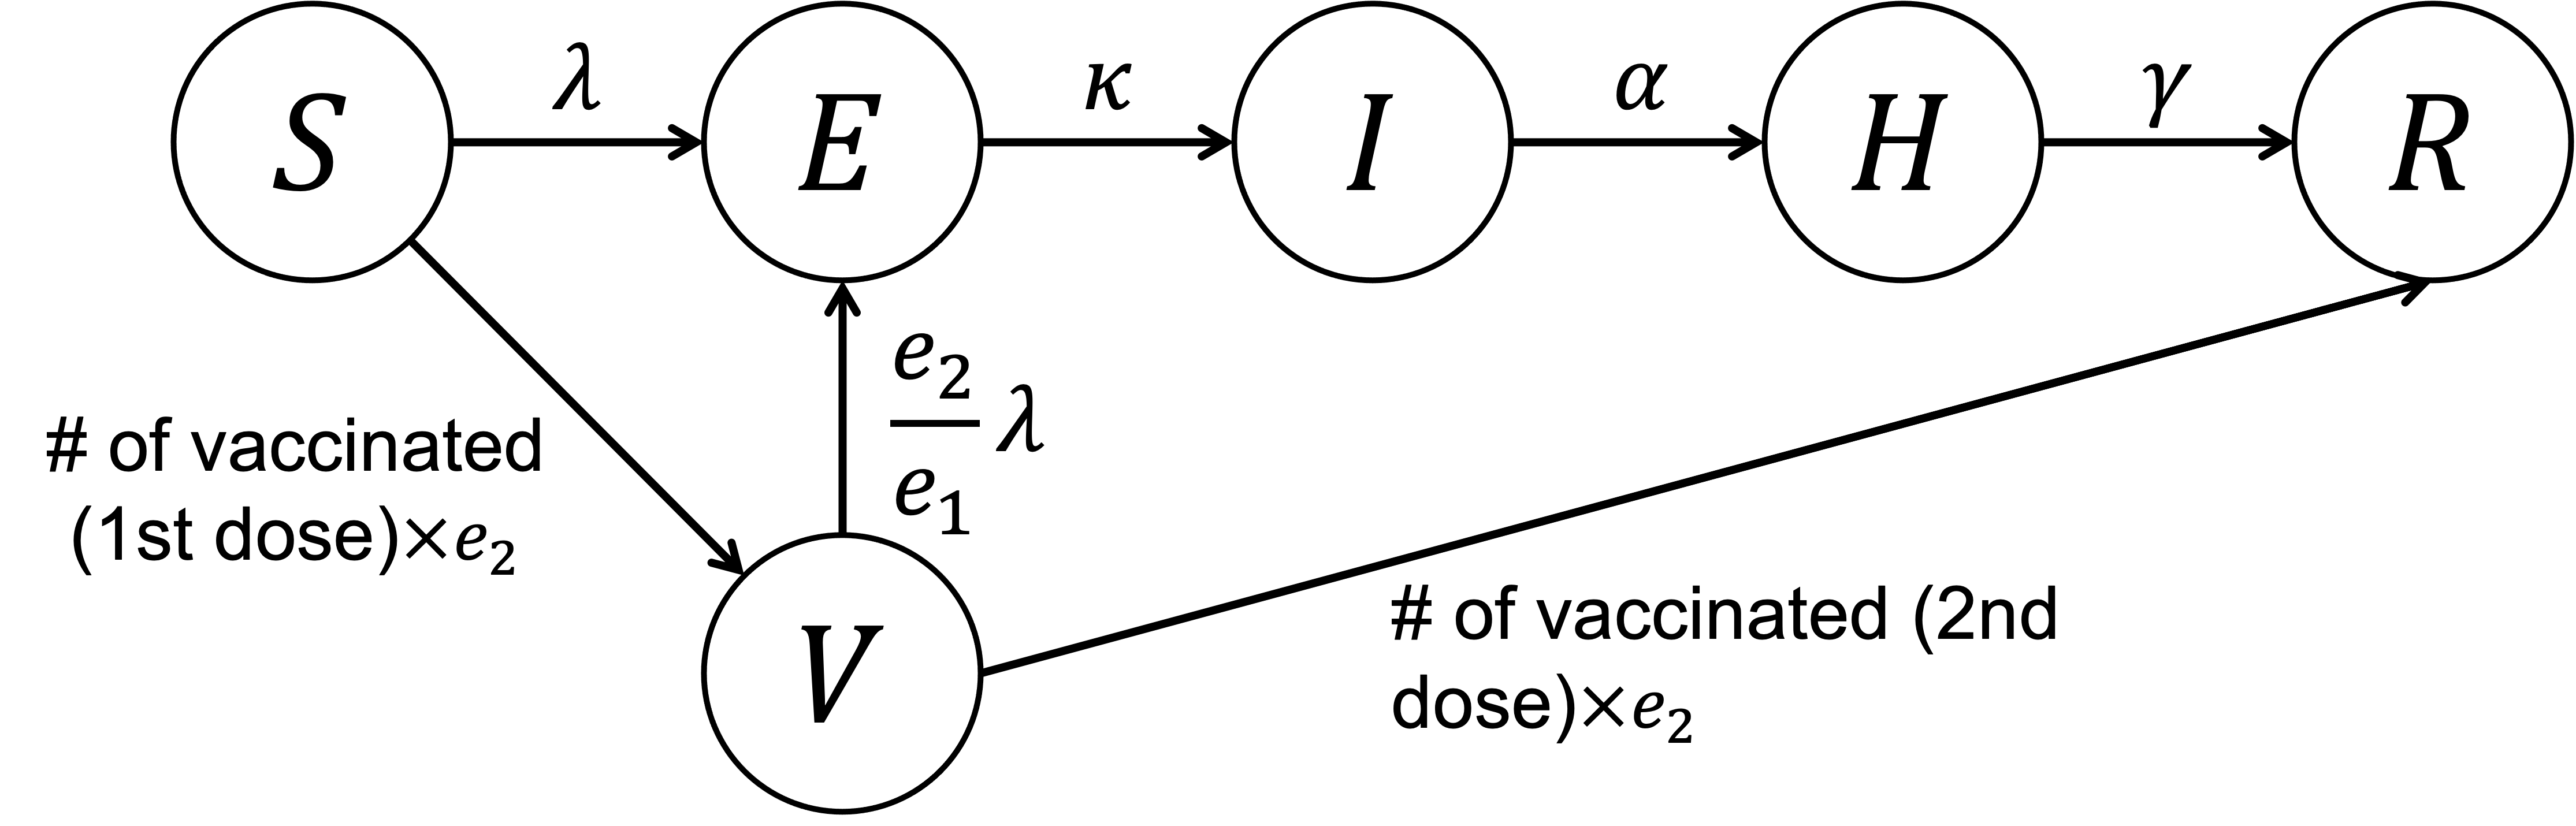
\includegraphics[width=12cm]{diagram.png}
	    	\caption{Diagram of age-structured model for SARS-CoV-2.}
	    \end{figure}
	\end{frame}

	\begin{frame}\frametitle{Model}
	    \begin{table}
	    	\begin{tabular}{cr}
	    		\toprule
	    		\textbf{Notation} & \textbf{Interpretation} \\
	    		\midrule
	    		$S$ & Susceptibles \\
	    		$E$ & Exposed \\
	    		$I$ & Infectious \\
	    		$H$ & Hospitalized \\
	    		$R$ & Removed (or recovered) \\
	    		$V$ & Vaccinated (between 1st dose and 2nd dose) \\
	    		$\lambda$ & Force of infection \\
	    		$\kappa$ & Latent period \\
	    		$\alpha$ & Infectious period \\
	    		$\gamma$ & Hospitalization period \\
	    		$e_1$ & Vaccine efficacy for 1st dose \\
	    		$e_2$ & Vaccine efficacy for 2nd dose \\
	    		\bottomrule
	    	\end{tabular}
	    	\caption{Definition of states and parameters.}
	    \end{table}
	\end{frame}

	\begin{frame}\frametitle{Social distancing}
		\textbf{Social distance level}
		\begin{itemize}
			\item 0.5단계 감소: transmission rate 전단계 대비 83.22\% 증가
			\item 0.5단계 증가: transmission rate 전단계 대비 30\% 감소
			\item 1단계 증가: transmission rate 전단계 대비 65\% 감소
		\end{itemize}
	    \begin{table}
	    	\begin{tabular}{ccr}
	    		\toprule
	    		\textbf{Date} & \textbf{Social distancing level} & \textbf{Change of transmission rate} \\
	    		\midrule
	    		2021/02/15-2021/06/30 & 2 &  \\
	    		2021/07/01-2021/07/11 & 1.5 & $\times 1.8322$ \\
	    		2021/07/12-2021/09/01 & 4 (assumed as 3 or 2.5 or 2) & $\times 0.699 \times 0.35$, $\times 0.35$, $\times 0.699$ \\
	    		\bottomrule
	    	\end{tabular}
	    	\caption{The change of transmission rate according to the social distancing level from 2021/02/15 to 2021/09/01.}
	    \end{table}
	\end{frame}

	\begin{frame}\frametitle{Definition of $\lambda$}
		\textbf{Motivation}
	    \begin{itemize}
	    	\item In general, $\lambda(t)$ is defined by $W \times I(t)$ where $W$ is the WAIFW matrix, and $I(t)$ is the number of infectious at time $t$.
	    	\item To reflect the non-pharmaceutical intervention, we consider time-dependent $W(t)$.
	    \end{itemize}
	    \vspace{0.5cm}
	    Let $p(t)$ and $SD(t)$ be the proportion of $\delta$ variant and proportionate of the corresponding social distancing level at time $t$.
	    \begin{enumerate}
	    	\item $W(t) = \left((1 - p(t) + p(t) \delta\right) \times \beta \times SD(t) \times C$
	    \end{enumerate}
	\end{frame}

	\begin{frame}\frametitle{Experiment}
		\textbf{Social distancing (2021/07/01-2021/07/11)}
	    \begin{itemize}
	    	\item 1.8322
	    	\item $1.4161 (:=1+0.8322/2)$
	    \end{itemize}
	    \vspace{0.5cm}
	    \textbf{Social distancing (2021/07/12-)}
	    \begin{itemize}
	    	\item 0.699 $\times$ 0.35
	    	\item 0.699
	    	\item 0.35
	    	\item $0.5245 (:= (0.699+0.35)/2)$
	    \end{itemize}
	\end{frame}

	\begin{frame}\frametitle{Experiment 1: 1st stage = $\beta \times 1.8322$, 2st stage = $\beta \times 1.8322 \times 0.699 \times 0.35$}
	    \begin{table}
	    	\begin{tabular}{crr}
	    		\toprule
	    		\textbf{Parameter} & \textbf{Initial} & \textbf{Estimate} \\
	    		\midrule
	    		$\delta$ & 1.0000e+00 & 2.4596e+00 \\
Cost & 7.4796e+04 & 2.0524e+04 \\
Time & 0.0000e+00 & 3.0104e+01 \\

	    		\bottomrule
	    	\end{tabular}
	    	\caption{Parameter estimates obtained by maximum likelihood estimation.}
	    \end{table}
	\end{frame}

	\begin{frame}\frametitle{Experiment 1: 1st stage = $\beta \times 1.8322$, 2st stage = $\beta \times 1.8322 \times 0.699 \times 0.35$}
	    \begin{figure}
	    	\centering
	    	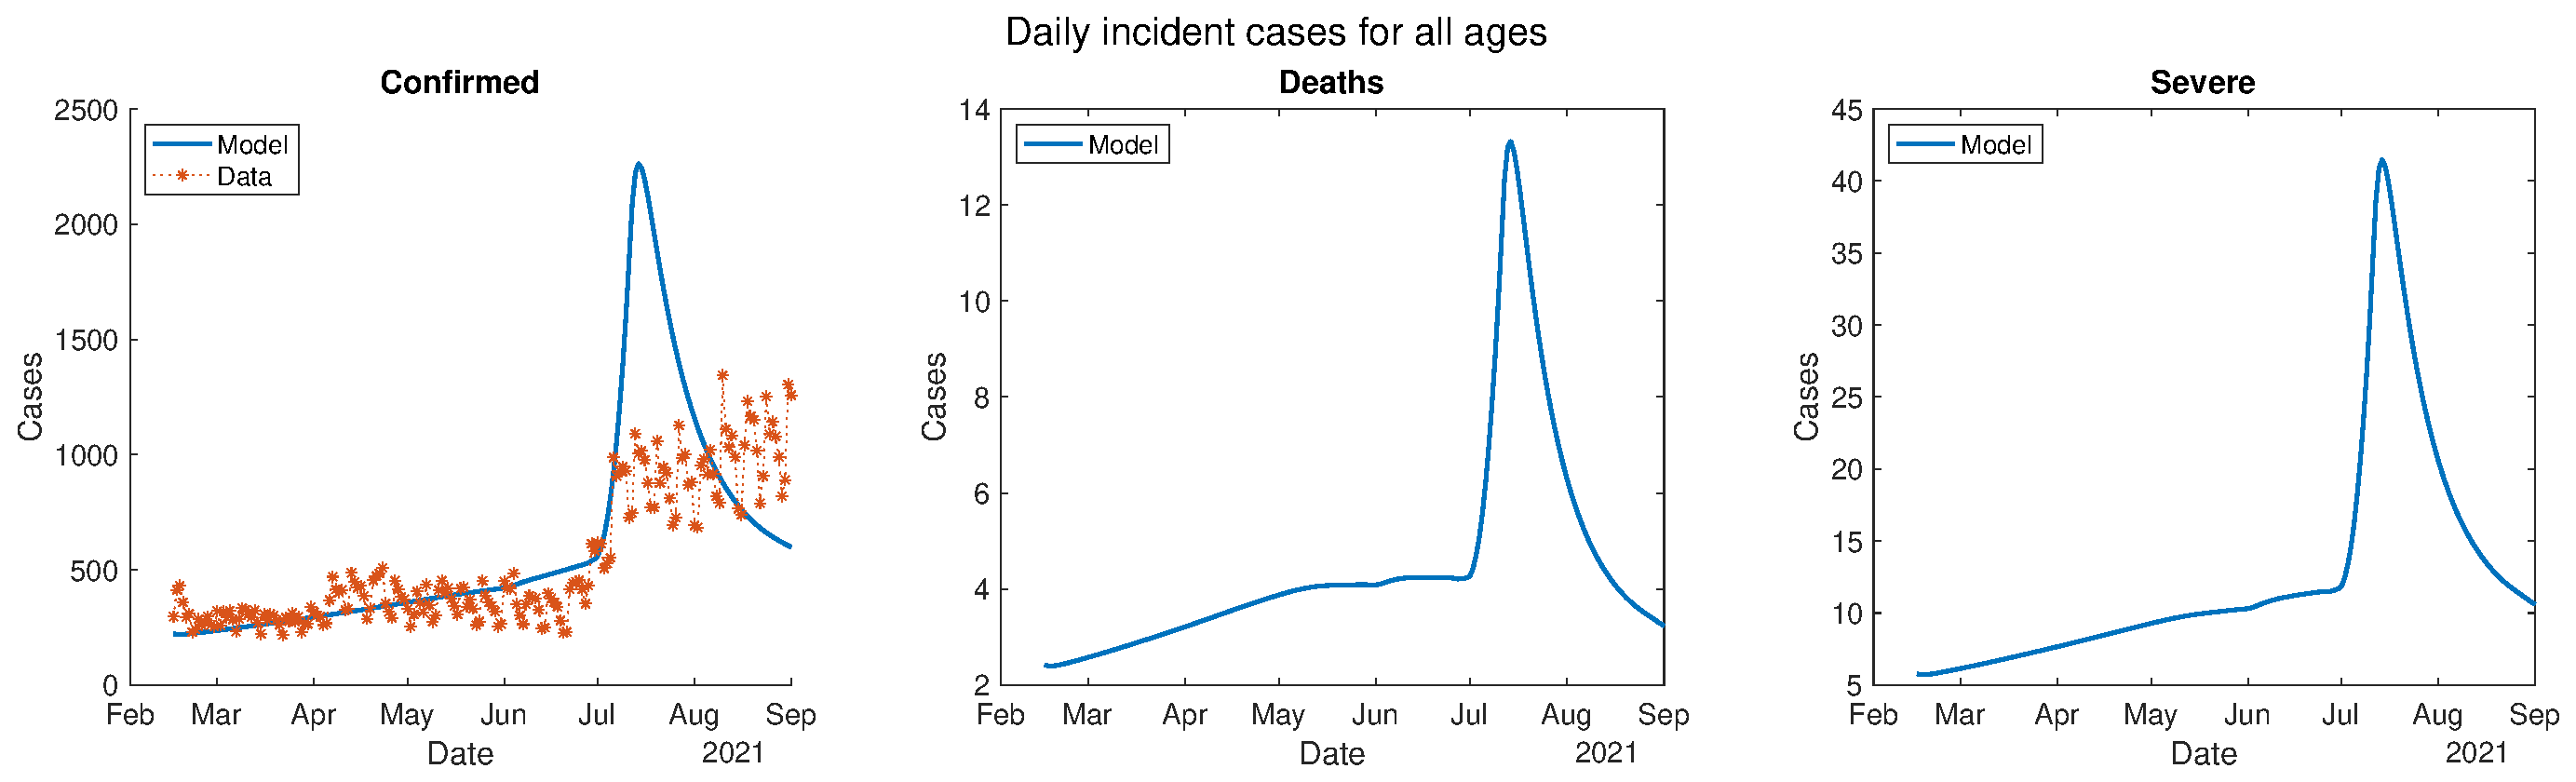
\includegraphics[width=11cm]{../results/estimate_sd_1st_1_2nd_1/daily_all_age.eps}
	    	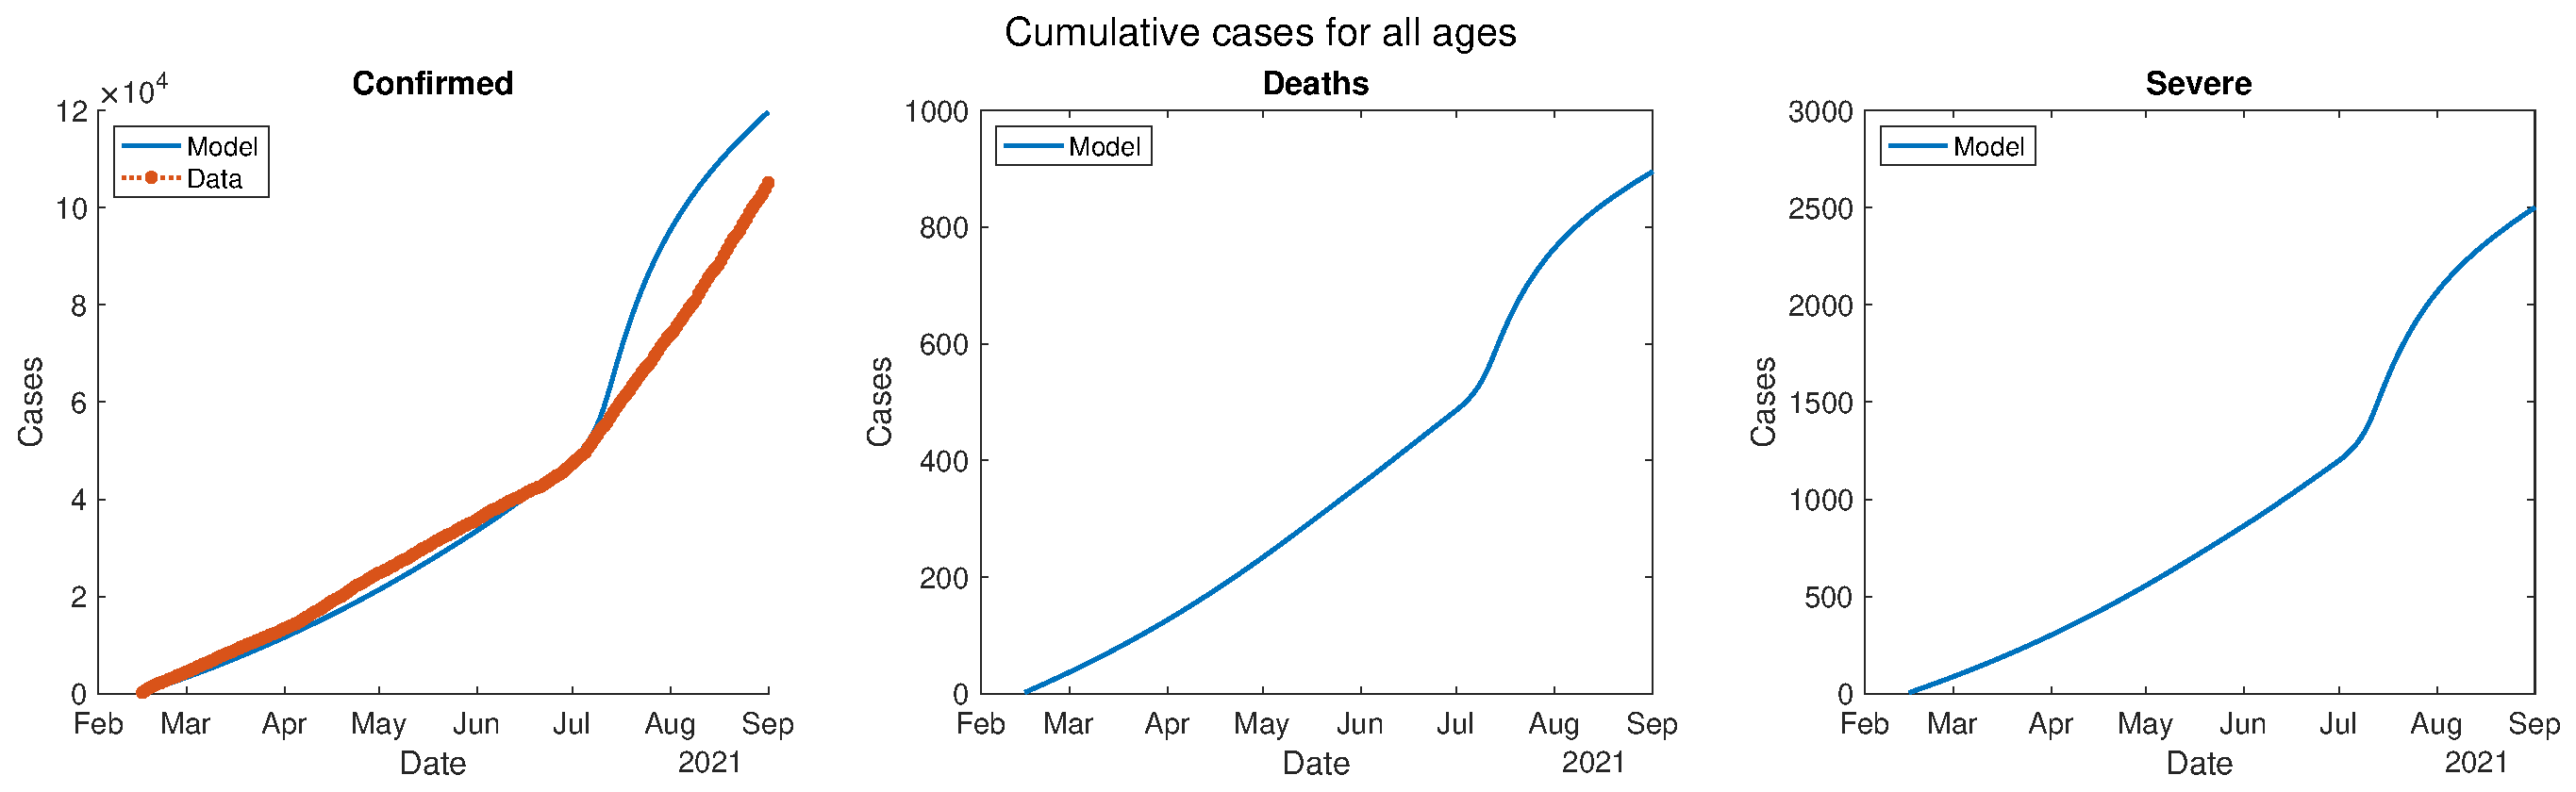
\includegraphics[width=11cm]{../results/estimate_sd_1st_1_2nd_1/cumul_all_age.eps}
	    	\caption{The model prediction and data for daily confirmed cases (top) and cumulative confirmed cases (bottom).}
	    \end{figure}
	\end{frame}

	\begin{frame}\frametitle{Experiment 1: 1st stage = $\beta \times 1.8322$, 2st stage = $\beta \times 1.8322 \times 0.699 \times 0.35$}
	    \begin{figure}
	    	\centering
	    	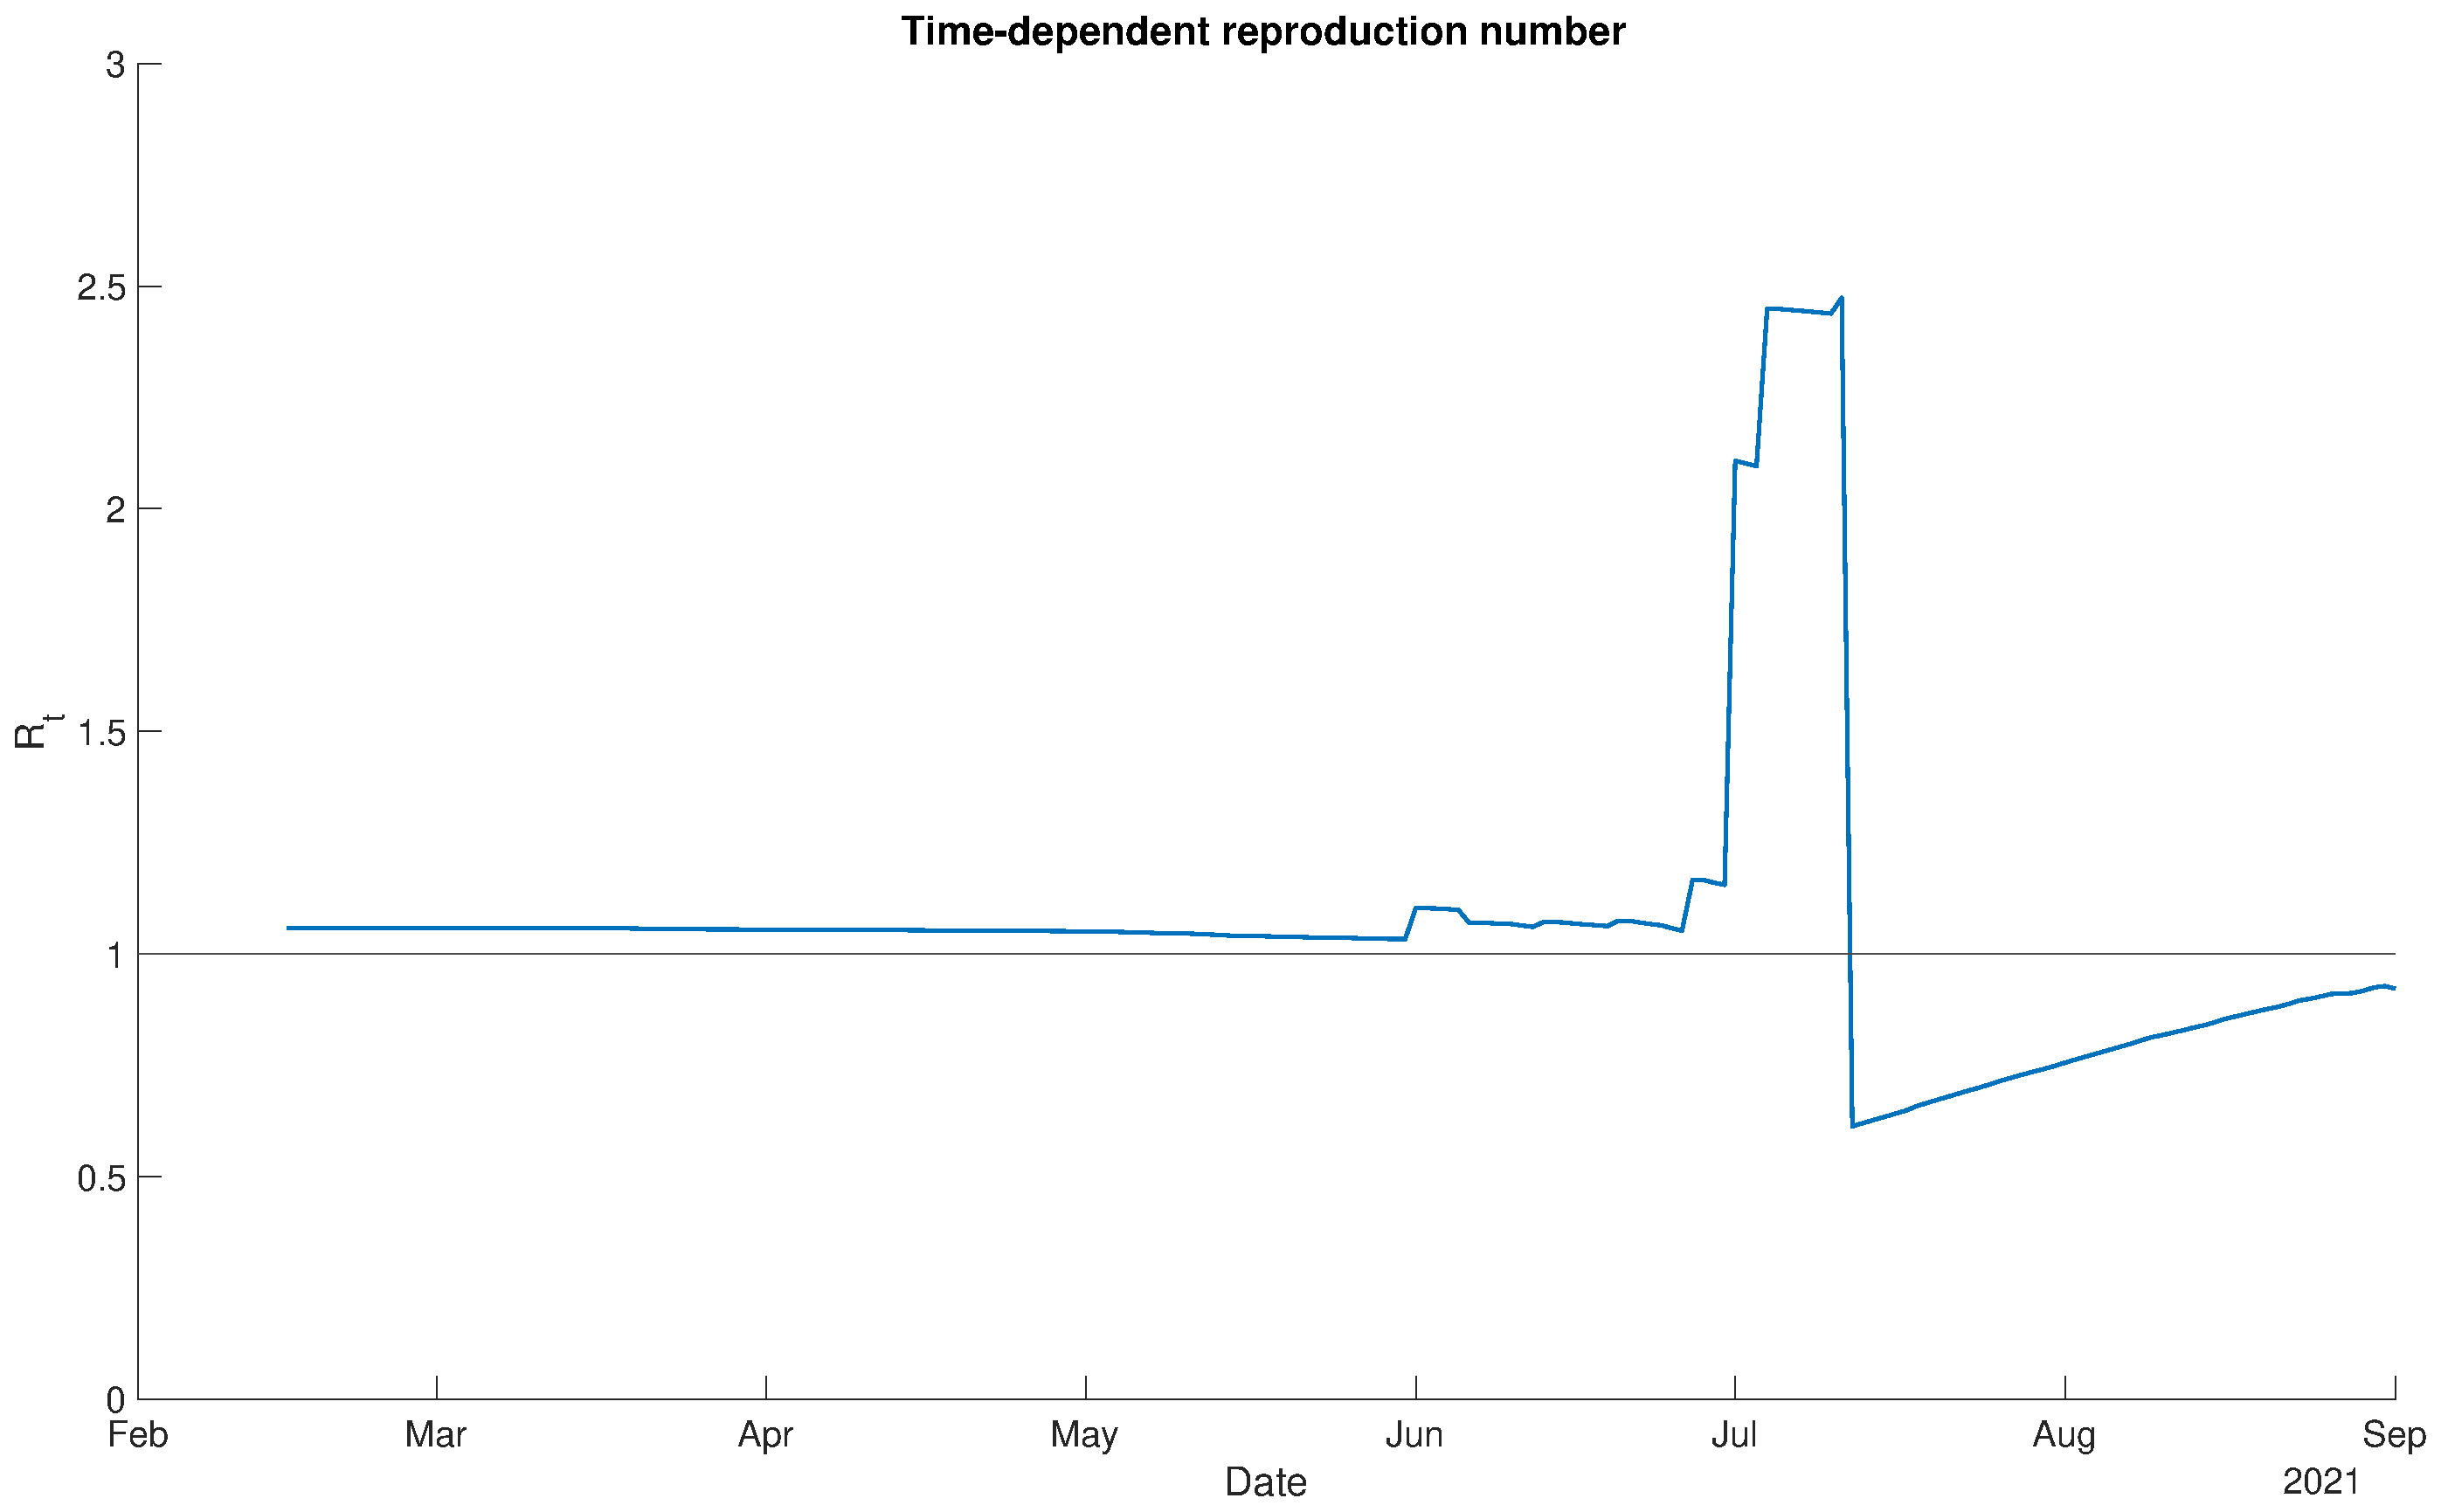
\includegraphics[width=10cm]{../results/estimate_sd_1st_1_2nd_1/rep_num.eps}
	    	\caption{The estimated reproduction number from 2021/02/15 to 2021/09/01.}
	    \end{figure}
	\end{frame}

	\begin{frame}\frametitle{Experiment 2: 1st stage = $\beta \times 1.8322$, 2st stage = $\beta \times 1.8322 \times 0.699$}
	    \begin{table}
	    	\begin{tabular}{crr}
	    		\toprule
	    		\textbf{Parameter} & \textbf{Initial} & \textbf{Estimate} \\
	    		\midrule
	    		$\delta$ & 1.0000e+00 & 1.0000e+00 \\
Cost & 3.5653e+04 & 3.5653e+04 \\
Time & 0.0000e+00 & 7.8846e+00 \\

	    		\bottomrule
	    	\end{tabular}
	    	\caption{Parameter estimates obtained by maximum likelihood estimation.}
	    \end{table}
	\end{frame}

	\begin{frame}\frametitle{Experiment 2: 1st stage = $\beta \times 1.8322$, 2st stage = $\beta \times 1.8322 \times 0.699$}
	    \begin{figure}
	    	\centering
	    	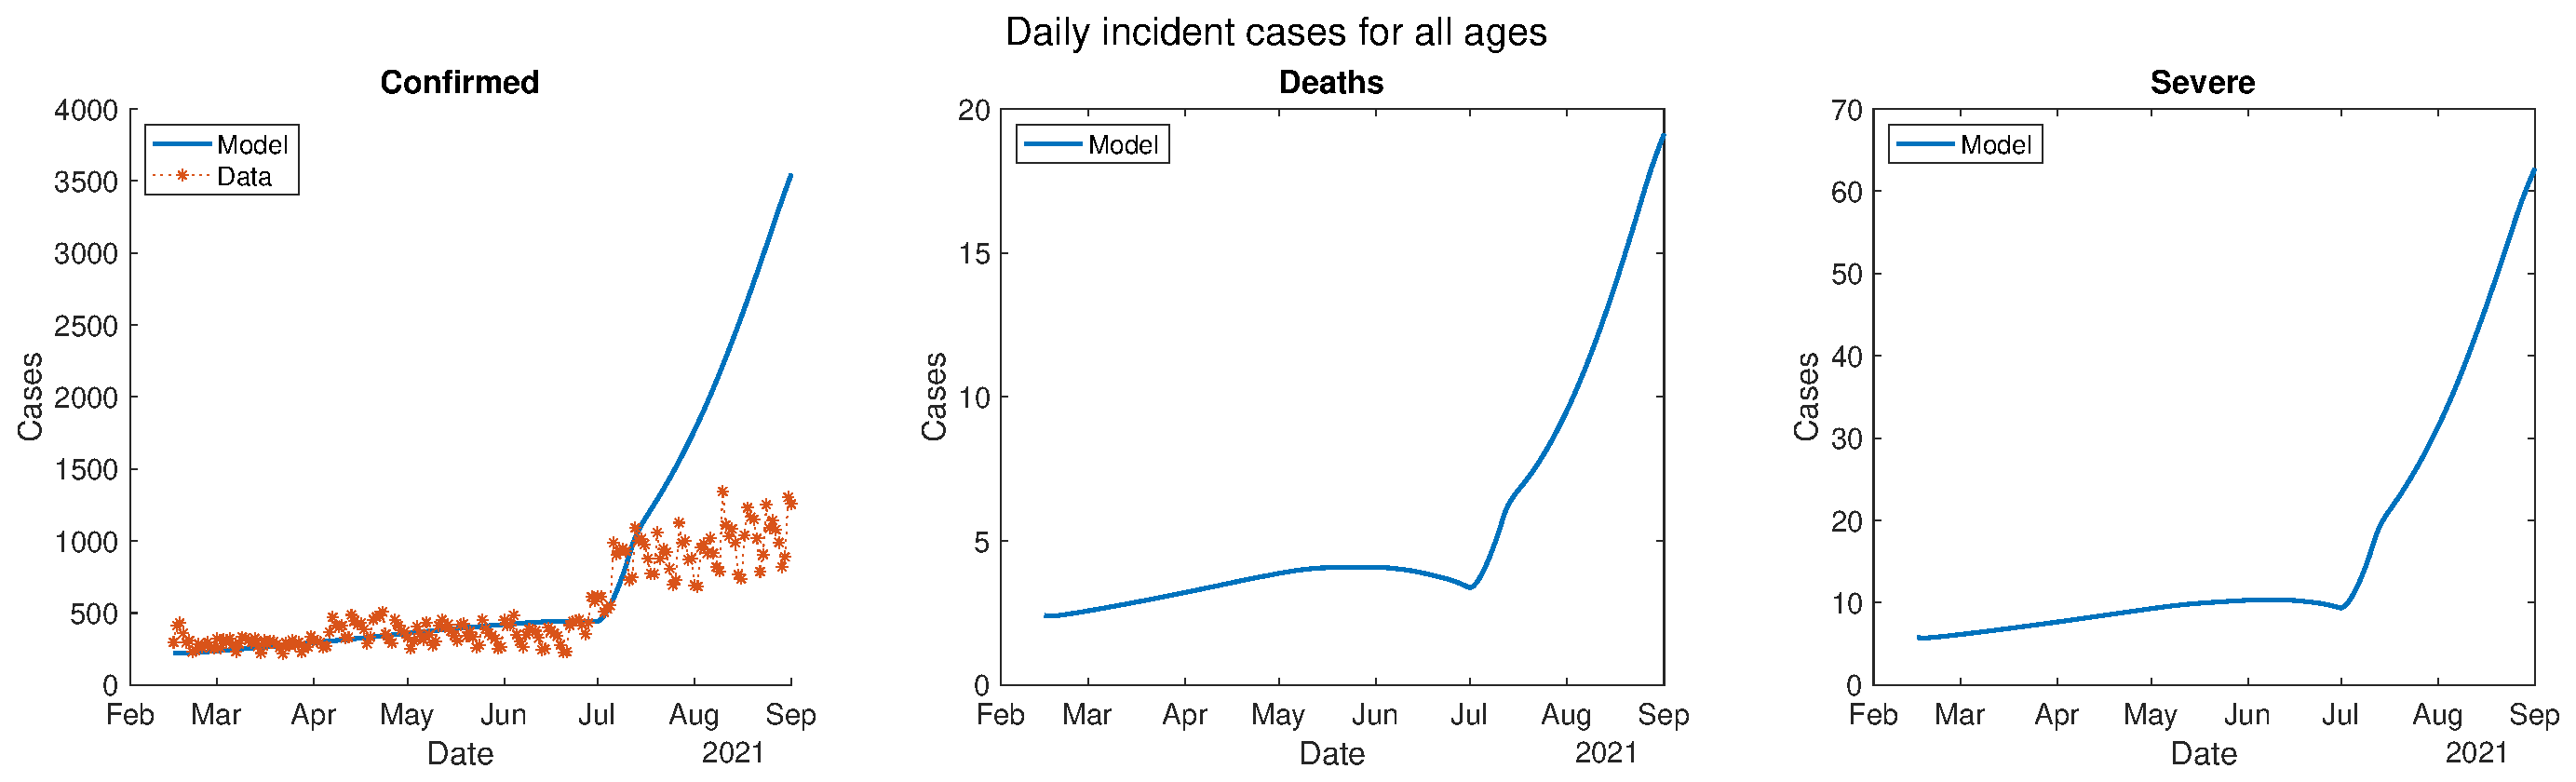
\includegraphics[width=11cm]{../results/estimate_sd_1st_1_2nd_2/daily_all_age.eps}
	    	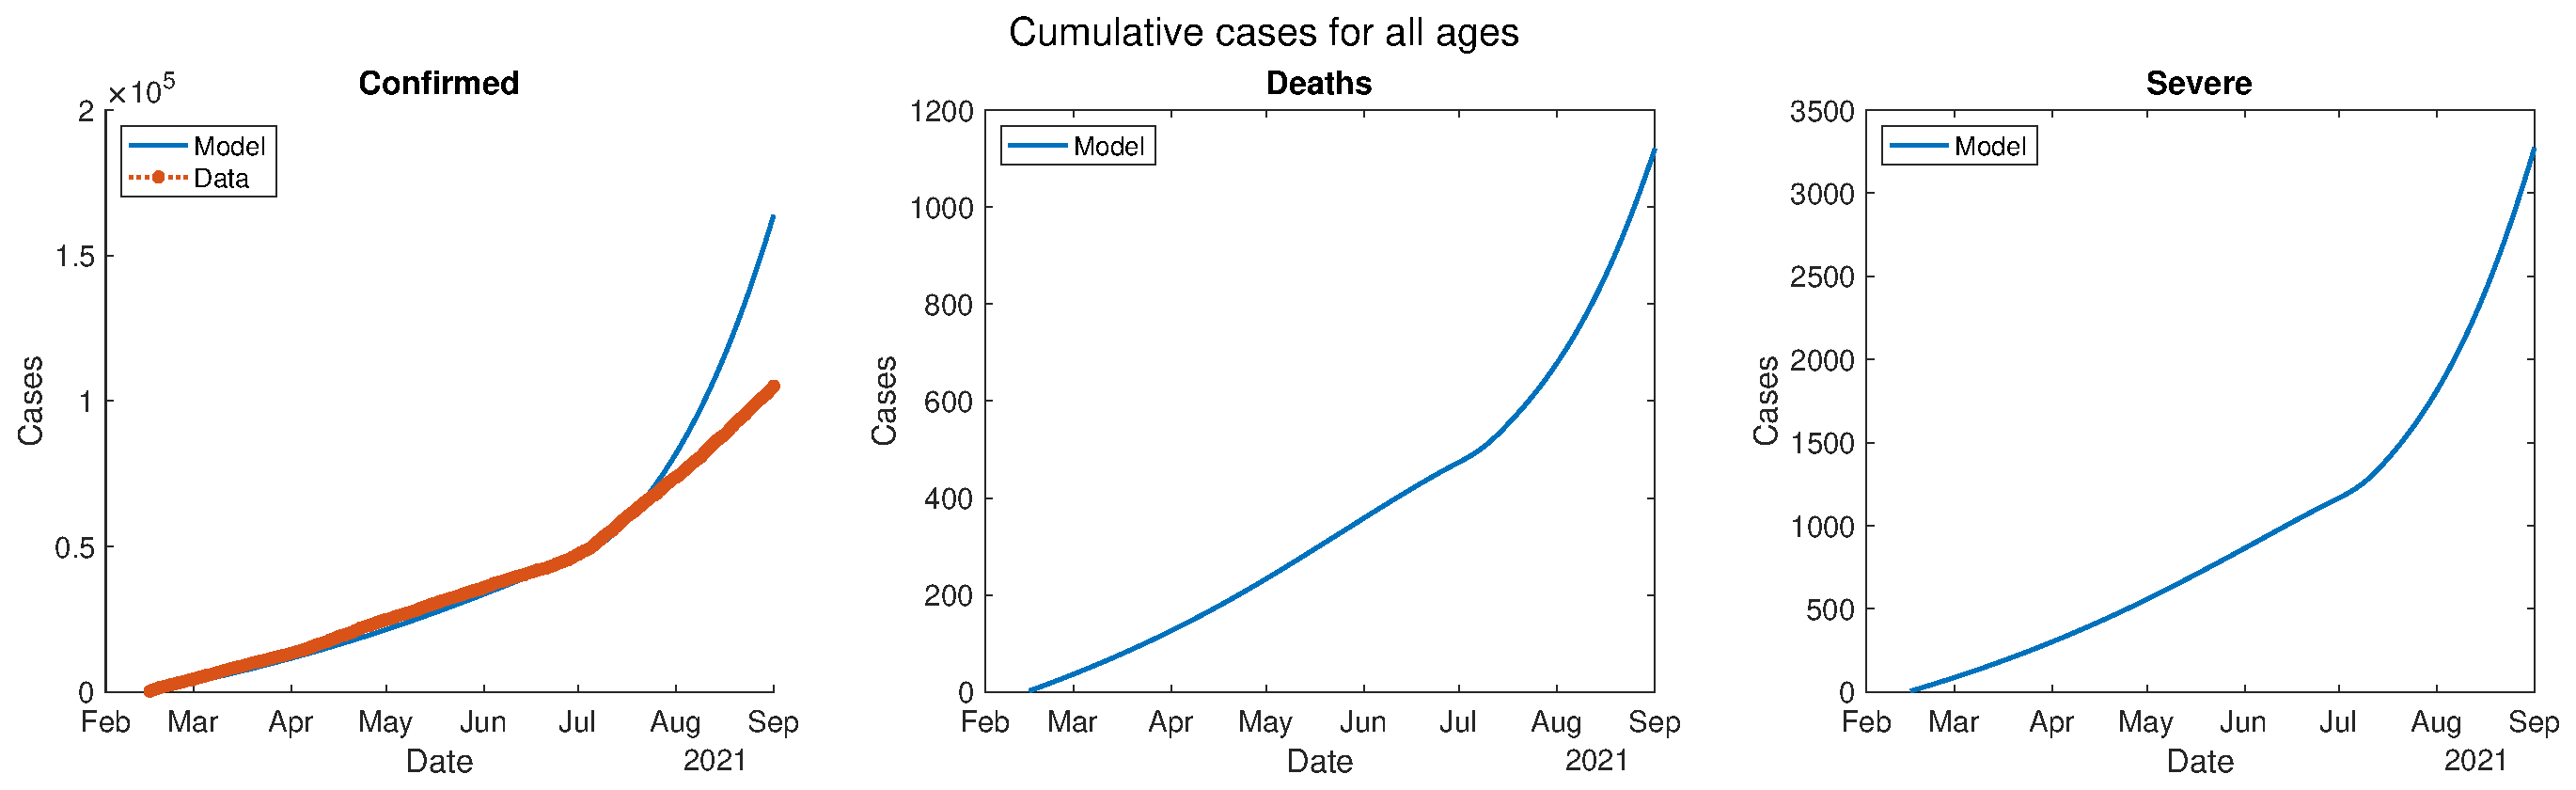
\includegraphics[width=11cm]{../results/estimate_sd_1st_1_2nd_2/cumul_all_age.eps}
	    	\caption{The model prediction and data for daily confirmed cases (top) and cumulative confirmed cases (bottom).}
	    \end{figure}
	\end{frame}

	\begin{frame}\frametitle{Experiment 2: 1st stage = $\beta \times 1.8322$, 2st stage = $\beta \times 1.8322 \times 0.699$}
	    \begin{figure}
	    	\centering
	    	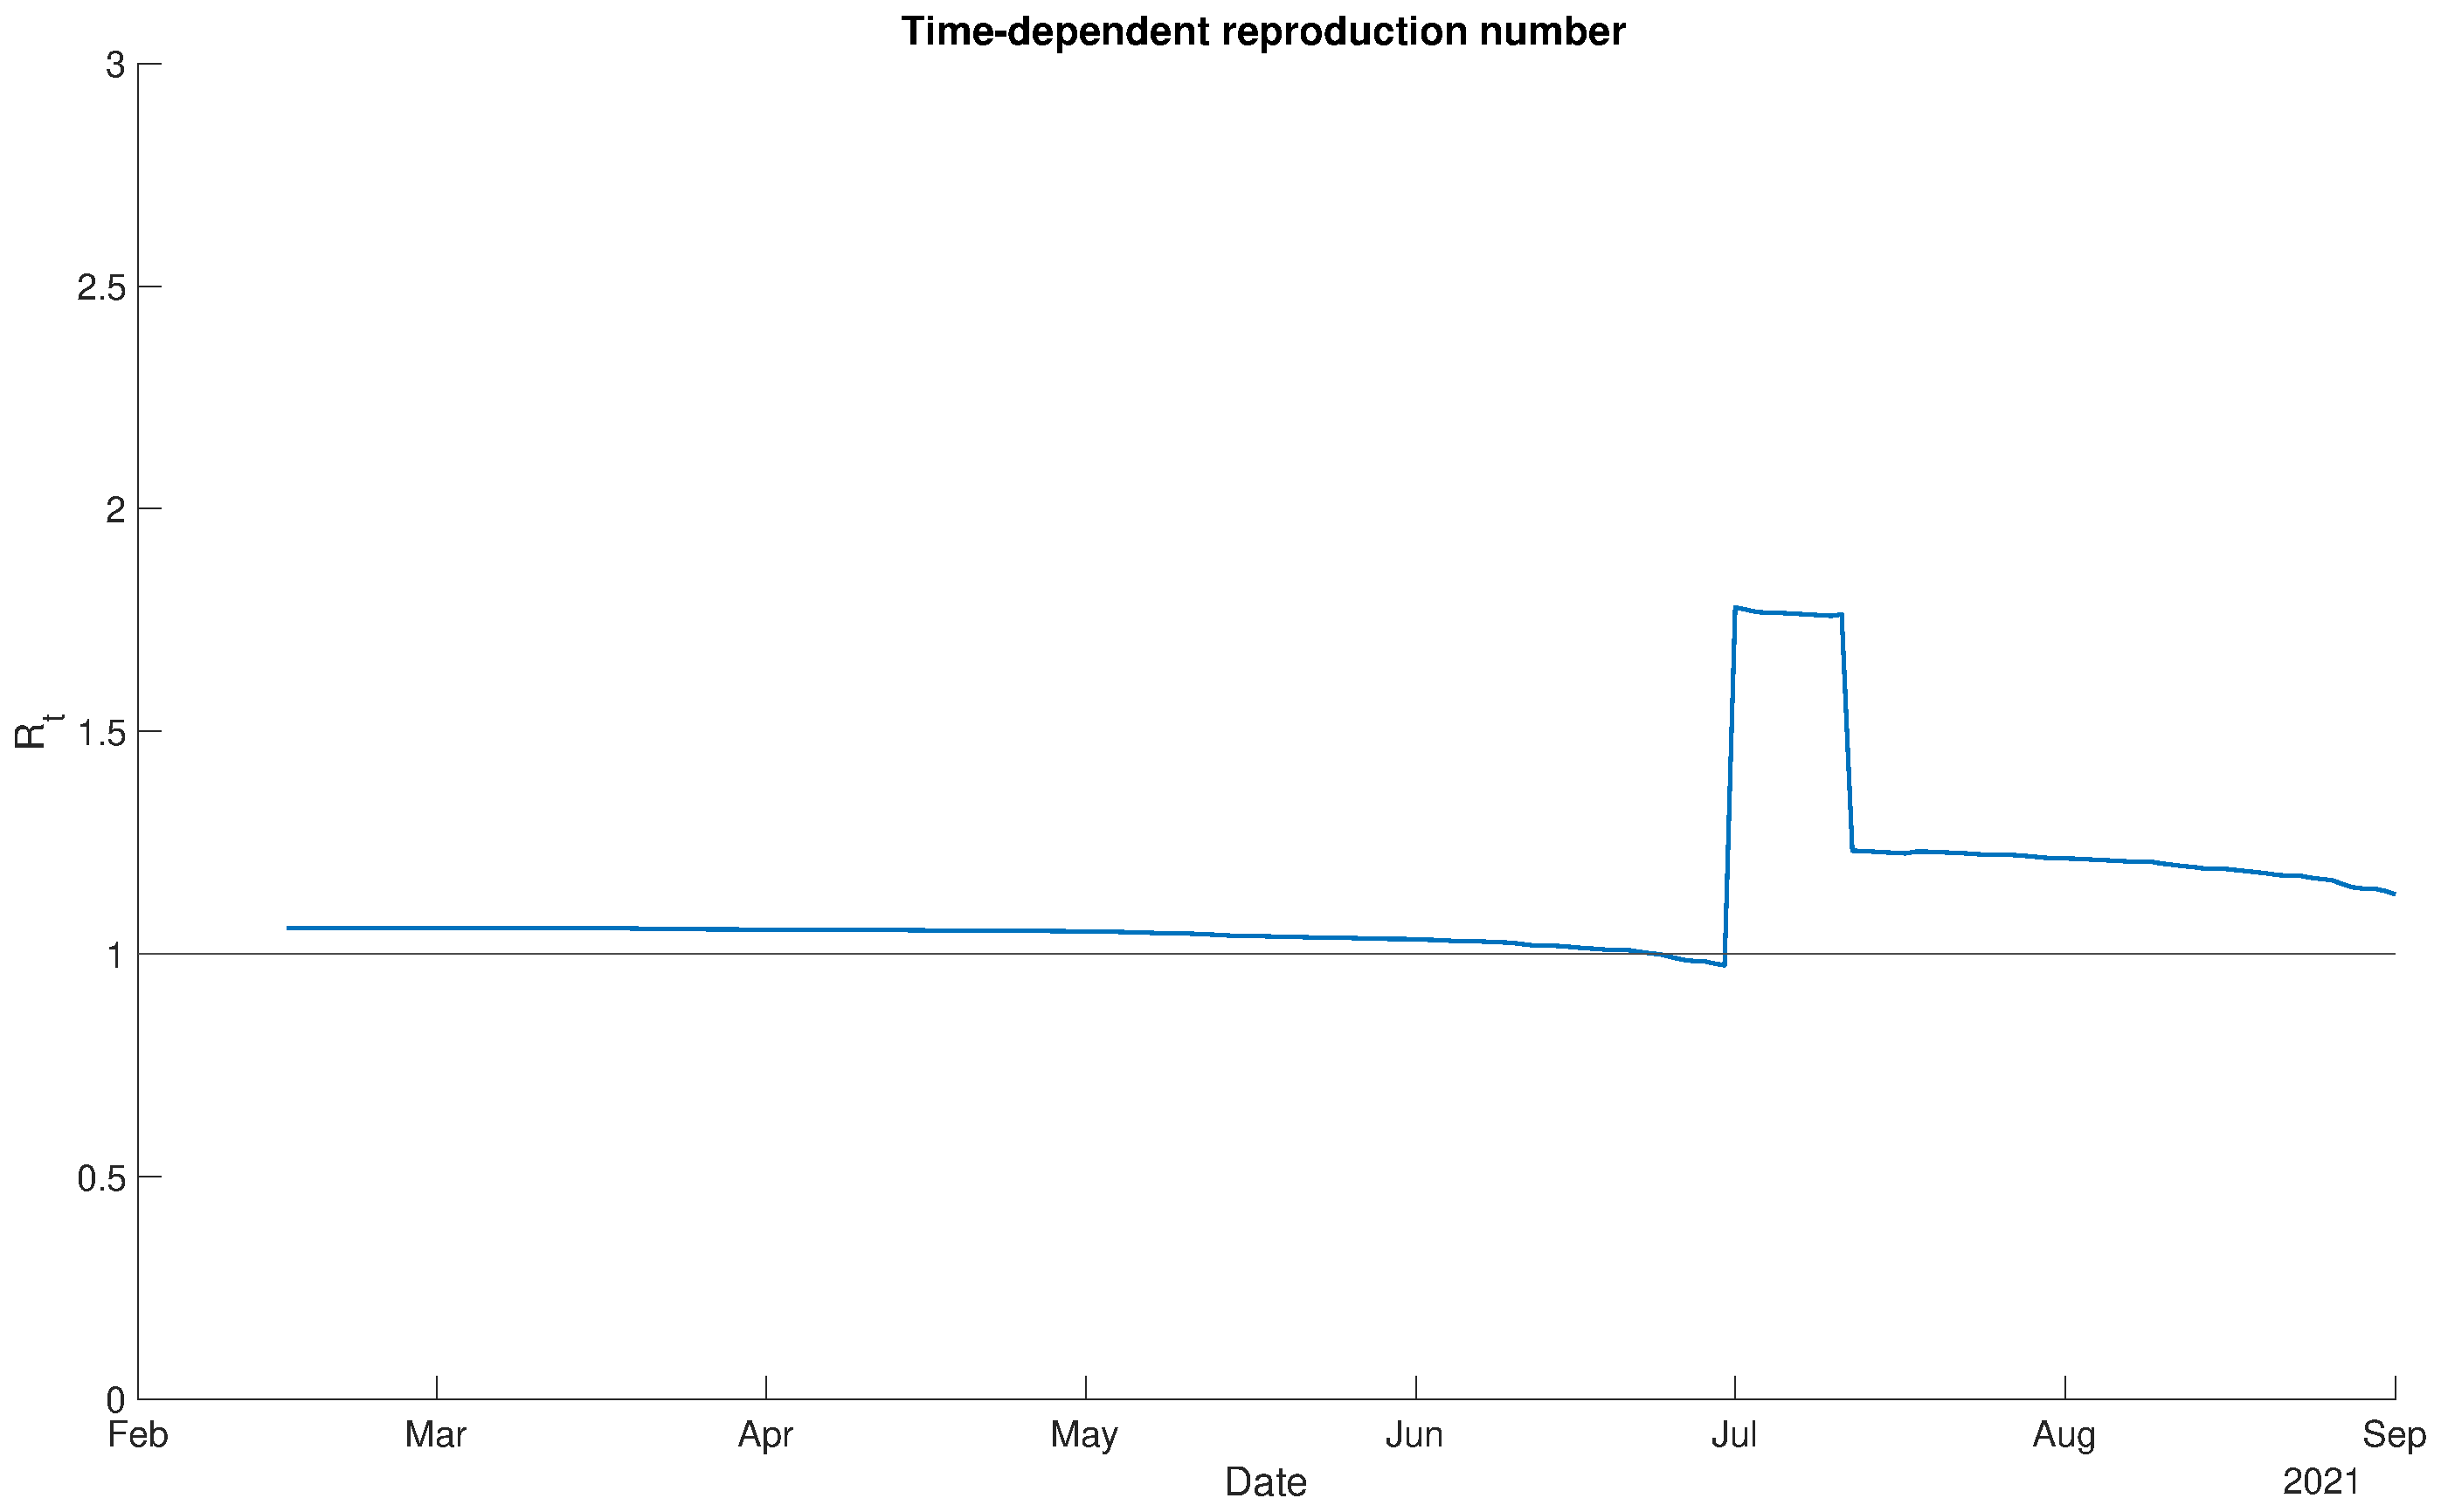
\includegraphics[width=10cm]{../results/estimate_sd_1st_1_2nd_2/rep_num.eps}
	    	\caption{The estimated reproduction number from 2021/02/15 to 2021/09/01.}
	    \end{figure}
	\end{frame}

	\begin{frame}\frametitle{Experiment 3: 1st stage = $\beta \times 1.8322$, 2st stage = $\beta \times 1.8322 \times 0.35$}
	    \begin{table}
	    	\begin{tabular}{crr}
	    		\toprule
	    		\textbf{Parameter} & \textbf{Initial} & \textbf{Estimate} \\
	    		\midrule
	    		$\delta$ & 1.0000e+00 & 1.7928e+00 \\
Cost & 4.5014e+04 & 1.5073e+04 \\
Time & 0.0000e+00 & 2.7888e+01 \\

	    		\bottomrule
	    	\end{tabular}
	    	\caption{Parameter estimates obtained by maximum likelihood estimation.}
	    \end{table}
	\end{frame}

	\begin{frame}\frametitle{Experiment 3: 1st stage = $\beta \times 1.8322$, 2st stage = $\beta \times 1.8322 \times 0.35$}
	    \begin{figure}
	    	\centering
	    	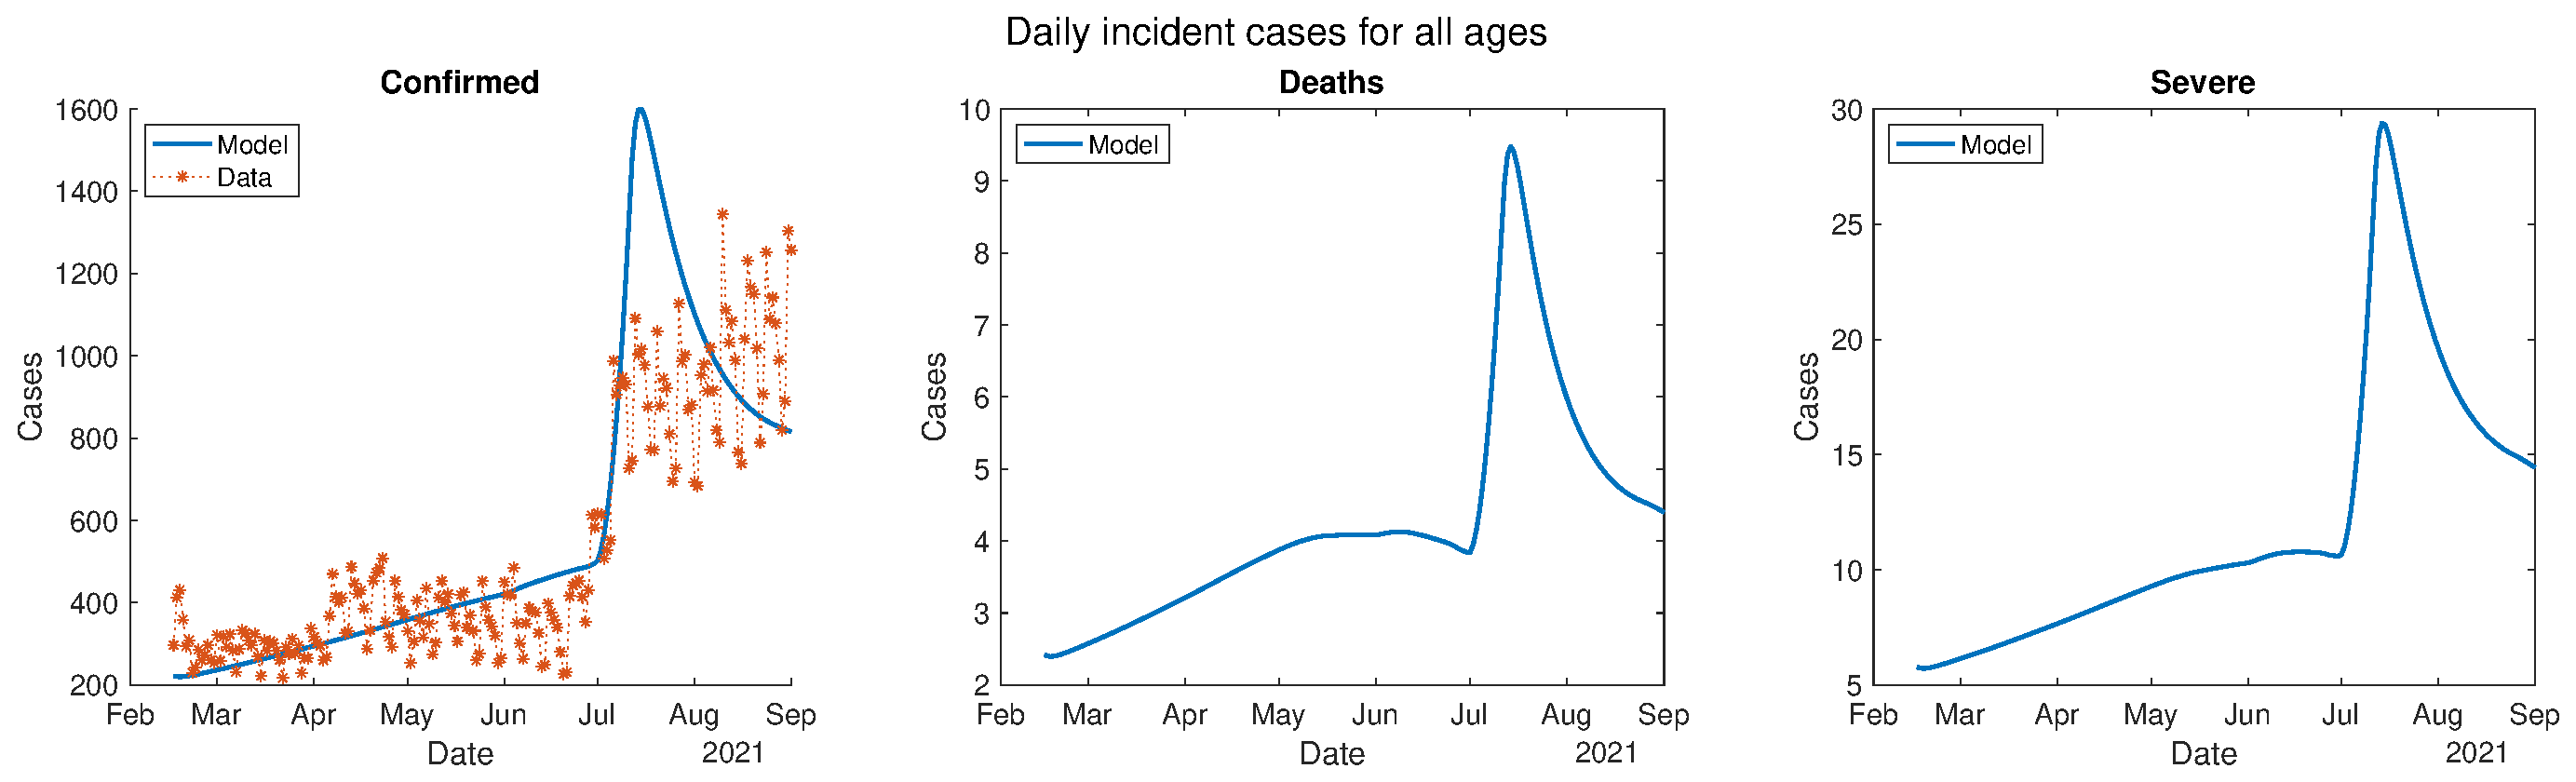
\includegraphics[width=11cm]{../results/estimate_sd_1st_1_2nd_3/daily_all_age.eps}
	    	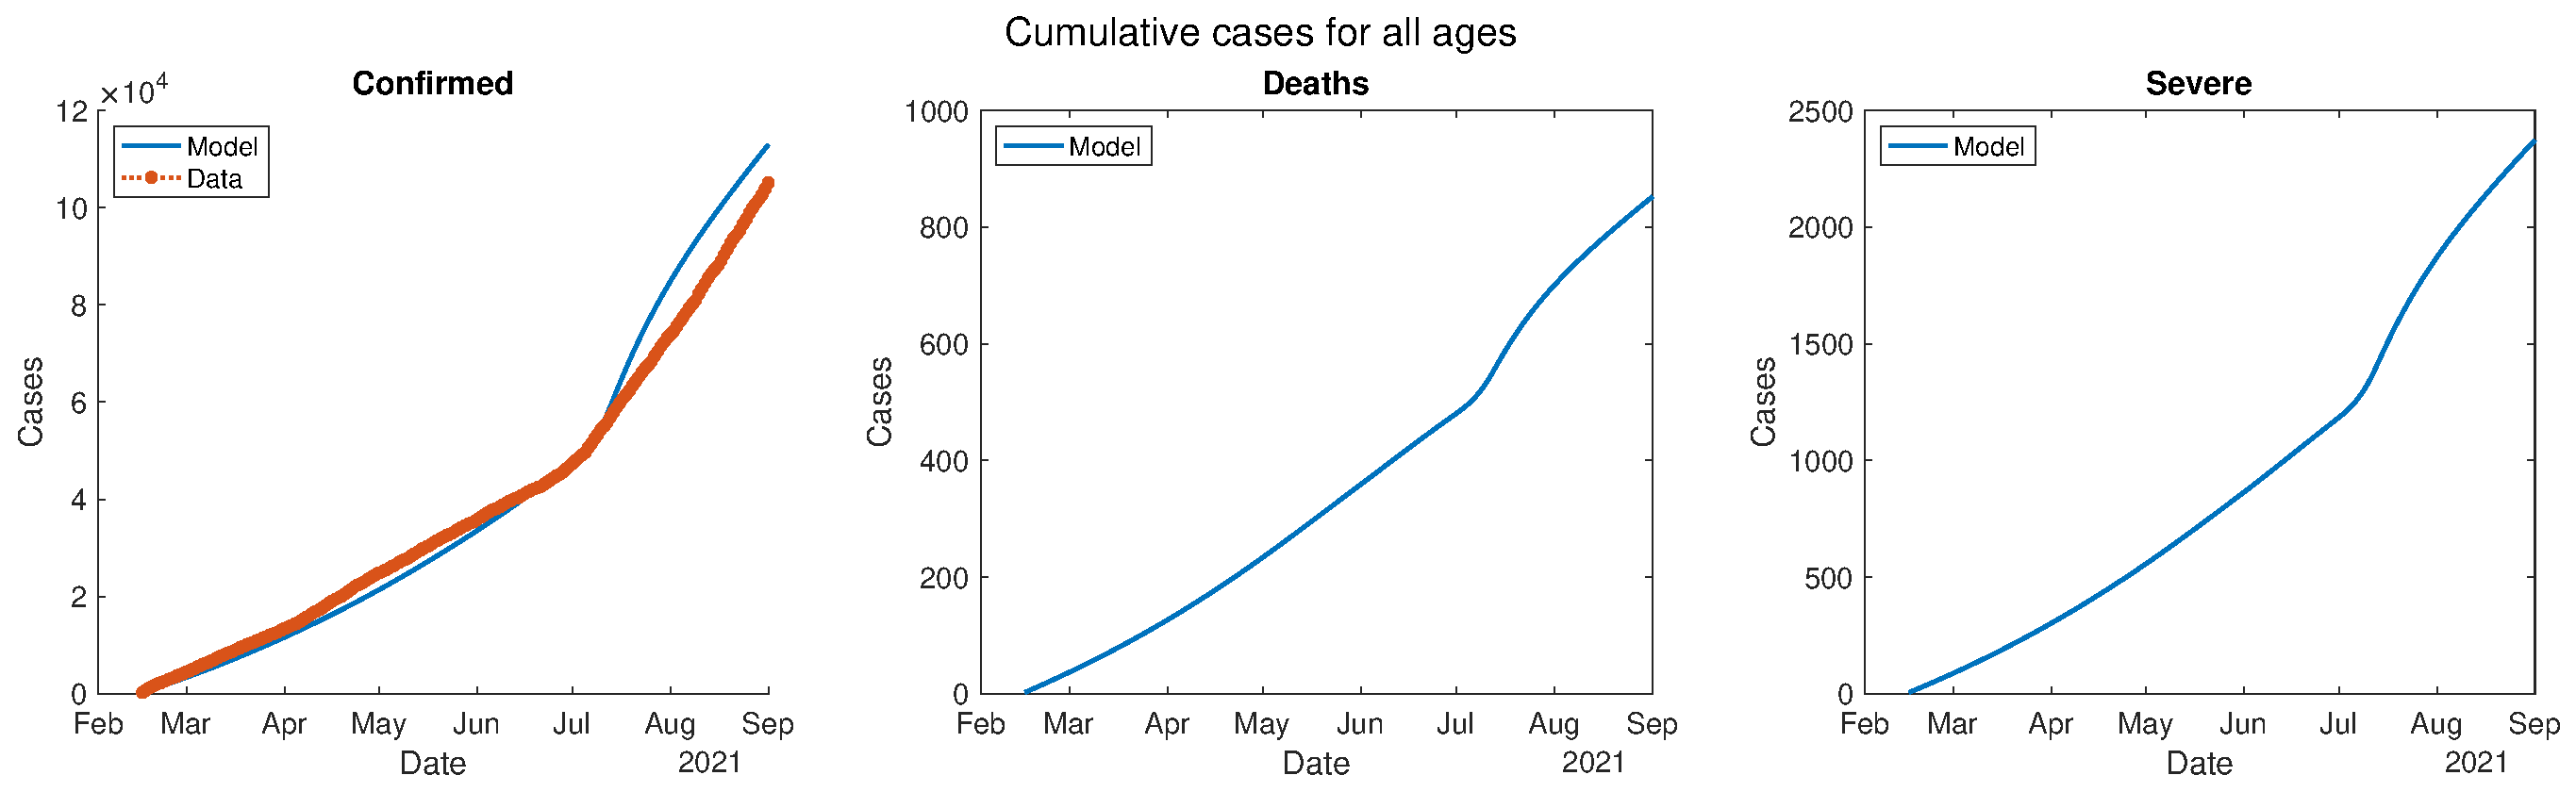
\includegraphics[width=11cm]{../results/estimate_sd_1st_1_2nd_3/cumul_all_age.eps}
	    	\caption{The model prediction and data for daily confirmed cases (top) and cumulative confirmed cases (bottom).}
	    \end{figure}
	\end{frame}

	\begin{frame}\frametitle{Experiment 3: 1st stage = $\beta \times 1.8322$, 2st stage = $\beta \times 1.8322 \times 0.35$}
	    \begin{figure}
	    	\centering
	    	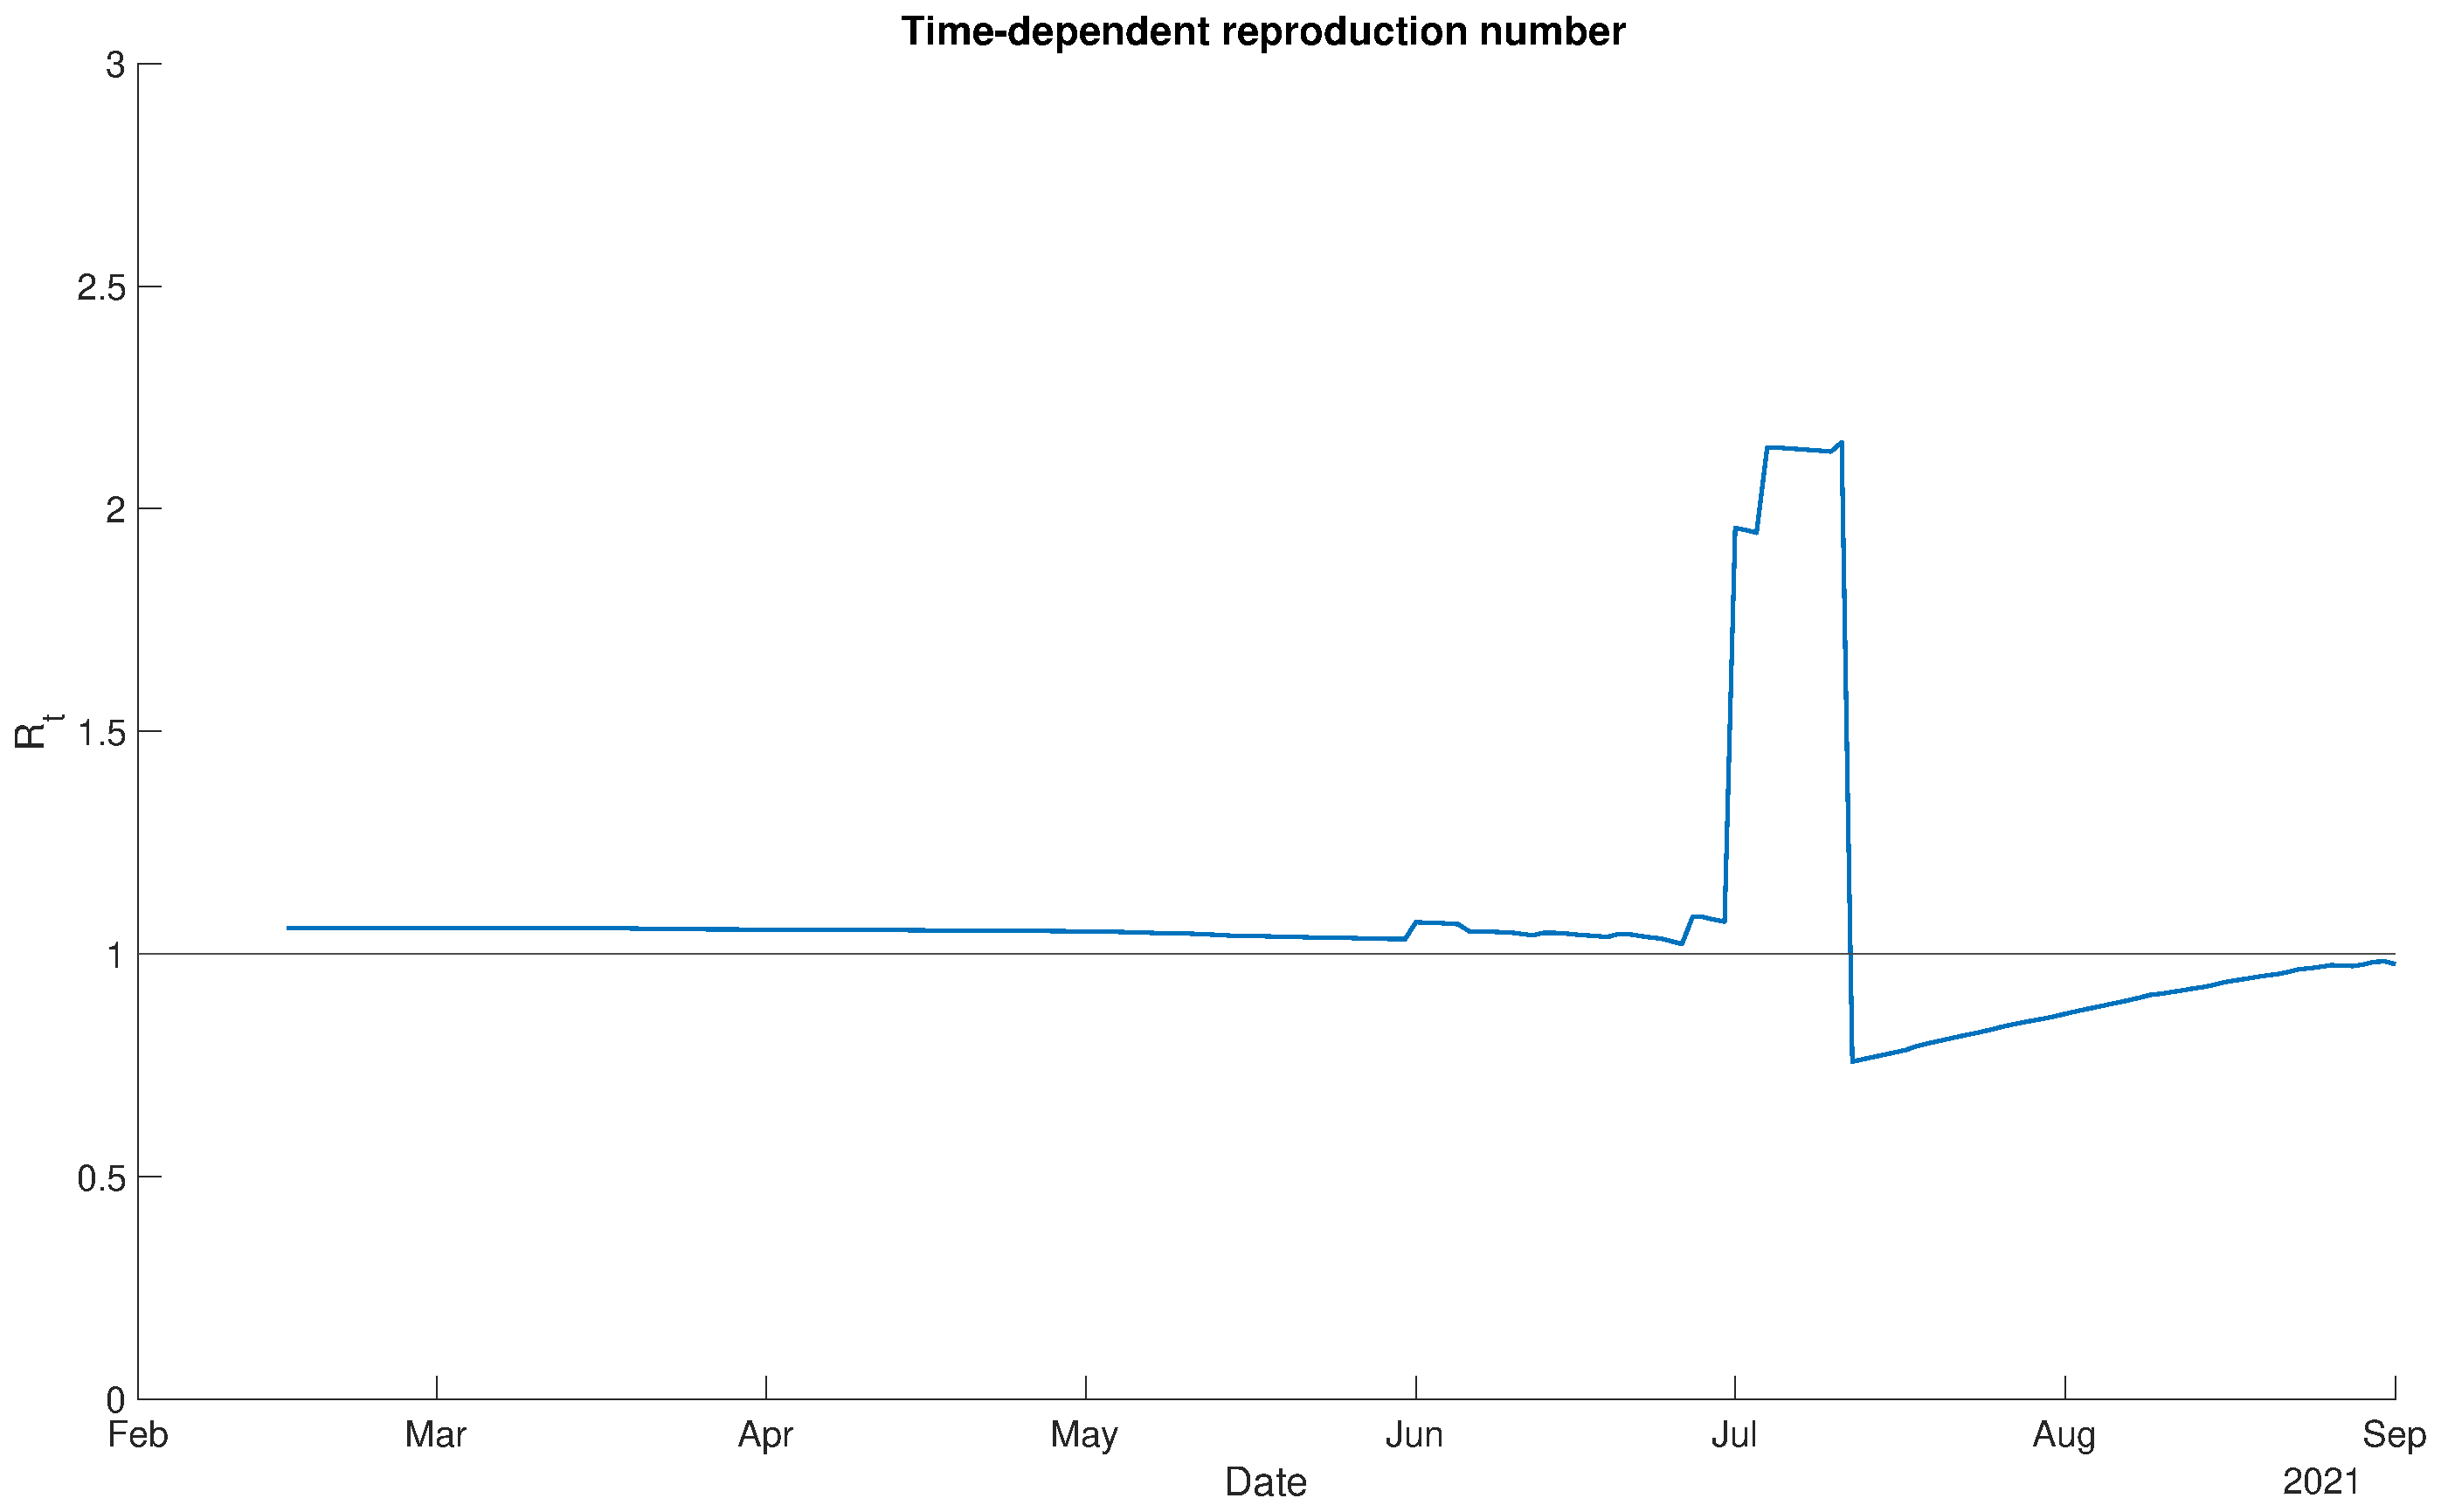
\includegraphics[width=10cm]{../results/estimate_sd_1st_1_2nd_3/rep_num.eps}
	    	\caption{The estimated reproduction number from 2021/02/15 to 2021/09/01.}
	    \end{figure}
	\end{frame}

	\begin{frame}\frametitle{Experiment 4: 1st stage = $\beta \times 1.8322$, 2st stage = $\beta \times 1.8322 \times 0.5245$}
	    \begin{table}
	    	\begin{tabular}{crr}
	    		\toprule
	    		\textbf{Parameter} & \textbf{Initial} & \textbf{Estimate} \\
	    		\midrule
	    		$\delta$ & 1.0000e+00 & 1.1112e+00 \\
Cost & 1.4410e+04 & 1.3009e+04 \\
Time & 0.0000e+00 & 2.3580e+01 \\

	    		\bottomrule
	    	\end{tabular}
	    	\caption{Parameter estimates obtained by maximum likelihood estimation.}
	    \end{table}
	\end{frame}

	\begin{frame}\frametitle{Experiment 4: 1st stage = $\beta \times 1.8322$, 2st stage = $\beta \times 1.8322 \times 0.5245$}
	    \begin{figure}
	    	\centering
	    	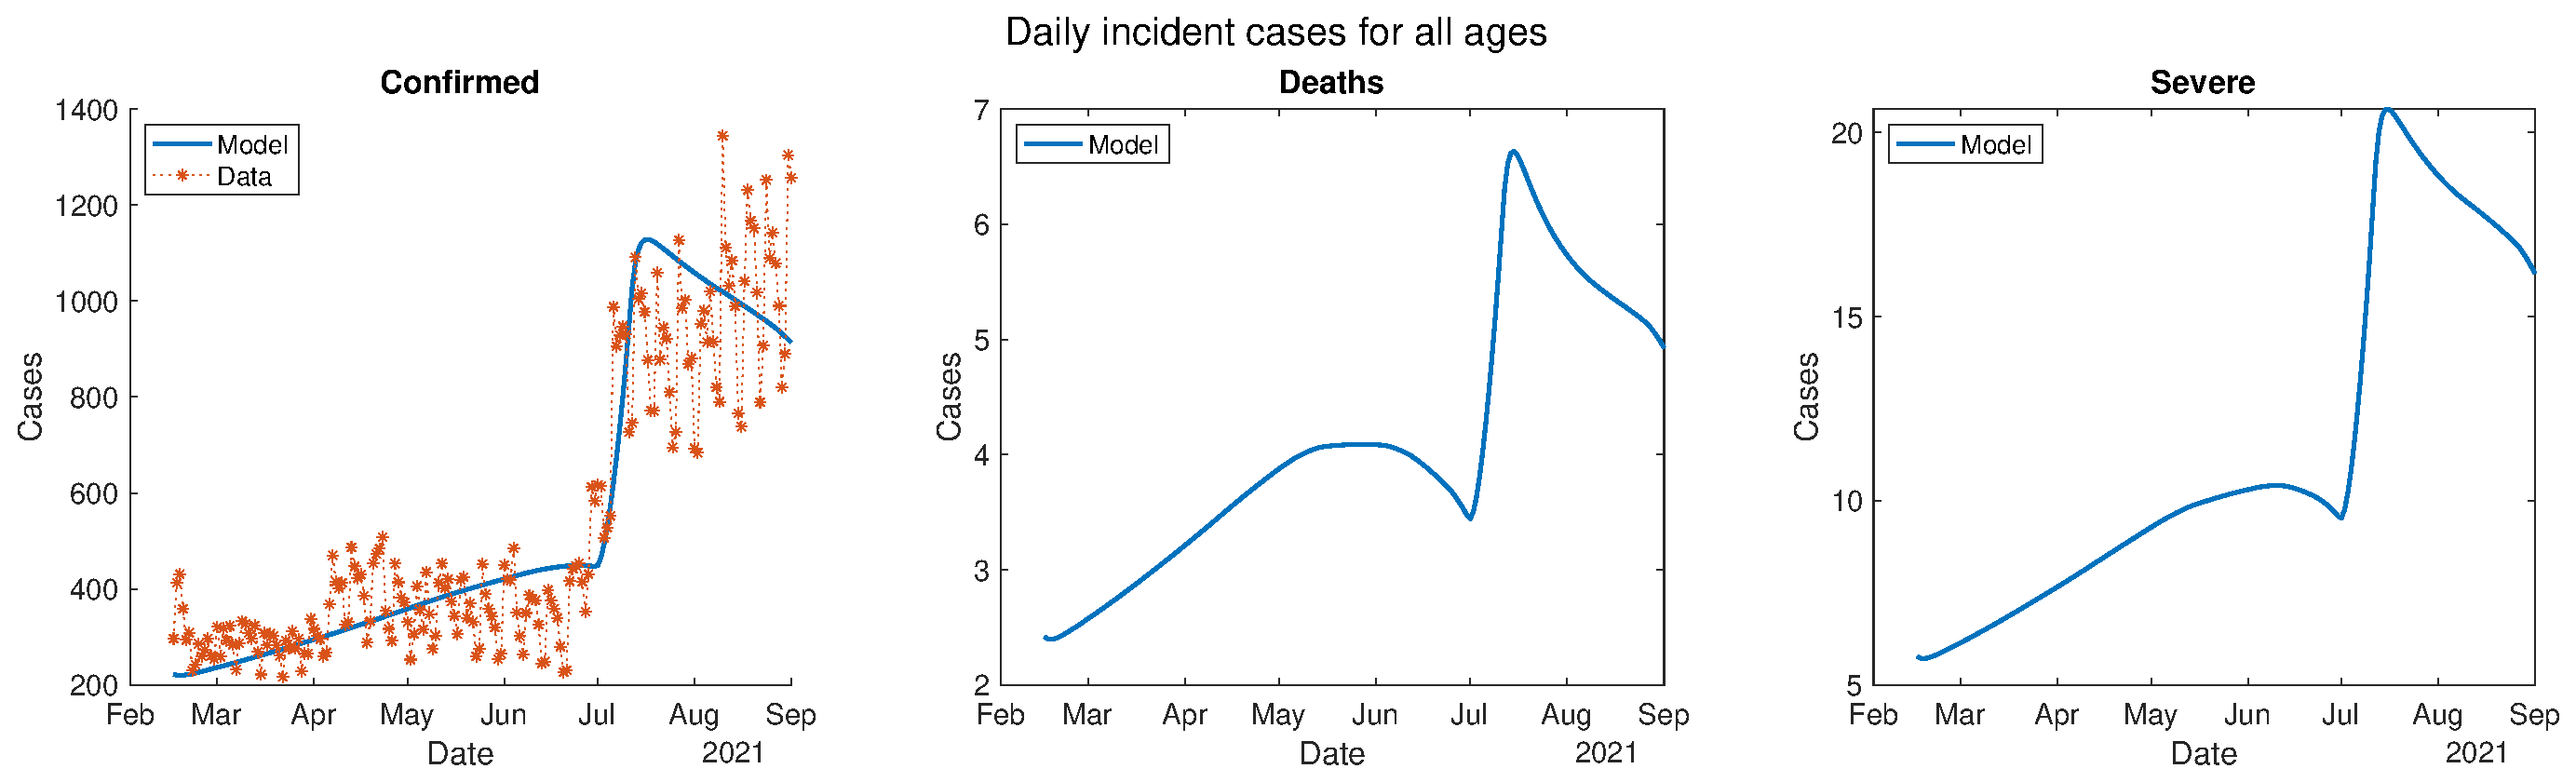
\includegraphics[width=11cm]{../results/estimate_sd_1st_1_2nd_4/daily_all_age.eps}
	    	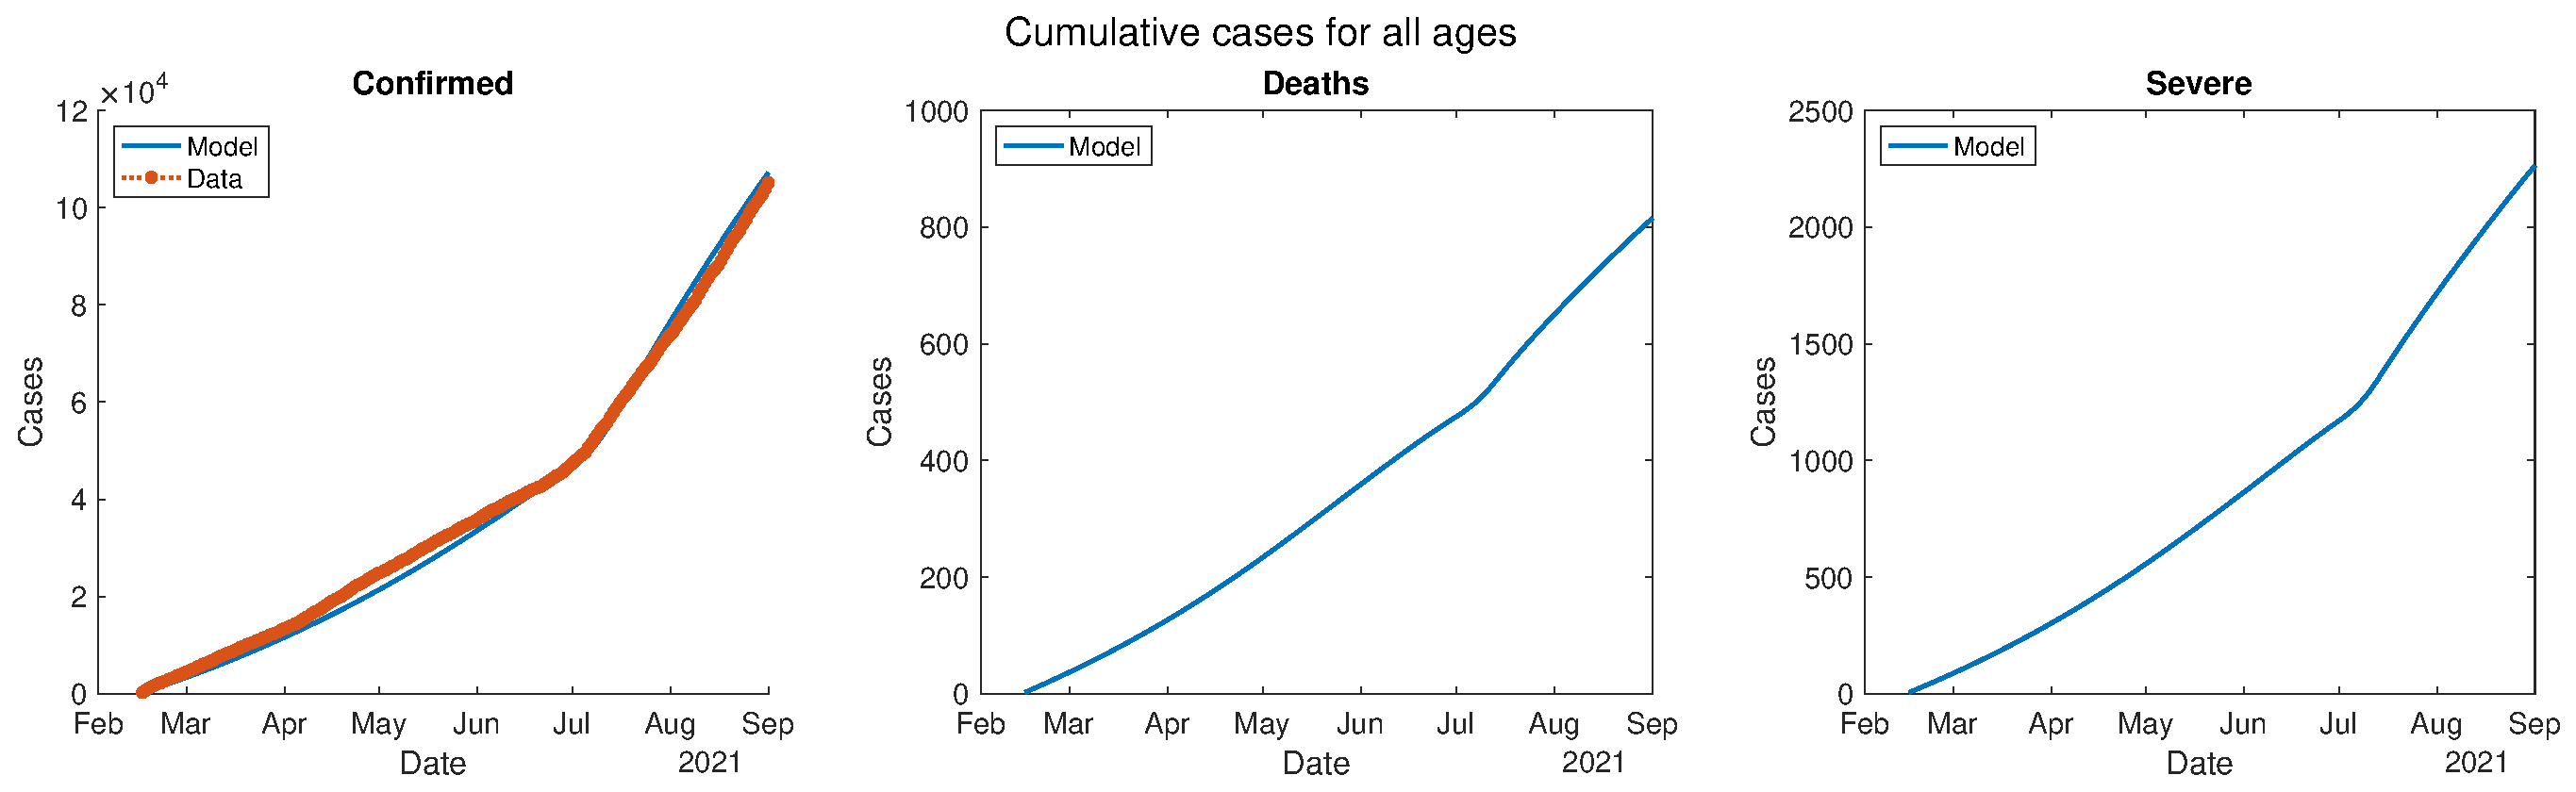
\includegraphics[width=11cm]{../results/estimate_sd_1st_1_2nd_4/cumul_all_age.eps}
	    	\caption{The model prediction and data for daily confirmed cases (top) and cumulative confirmed cases (bottom).}
	    \end{figure}
	\end{frame}

	\begin{frame}\frametitle{Experiment 4: 1st stage = $\beta \times 1.8322$, 2st stage = $\beta \times 1.8322 \times 0.5245$}
	    \begin{figure}
	    	\centering
	    	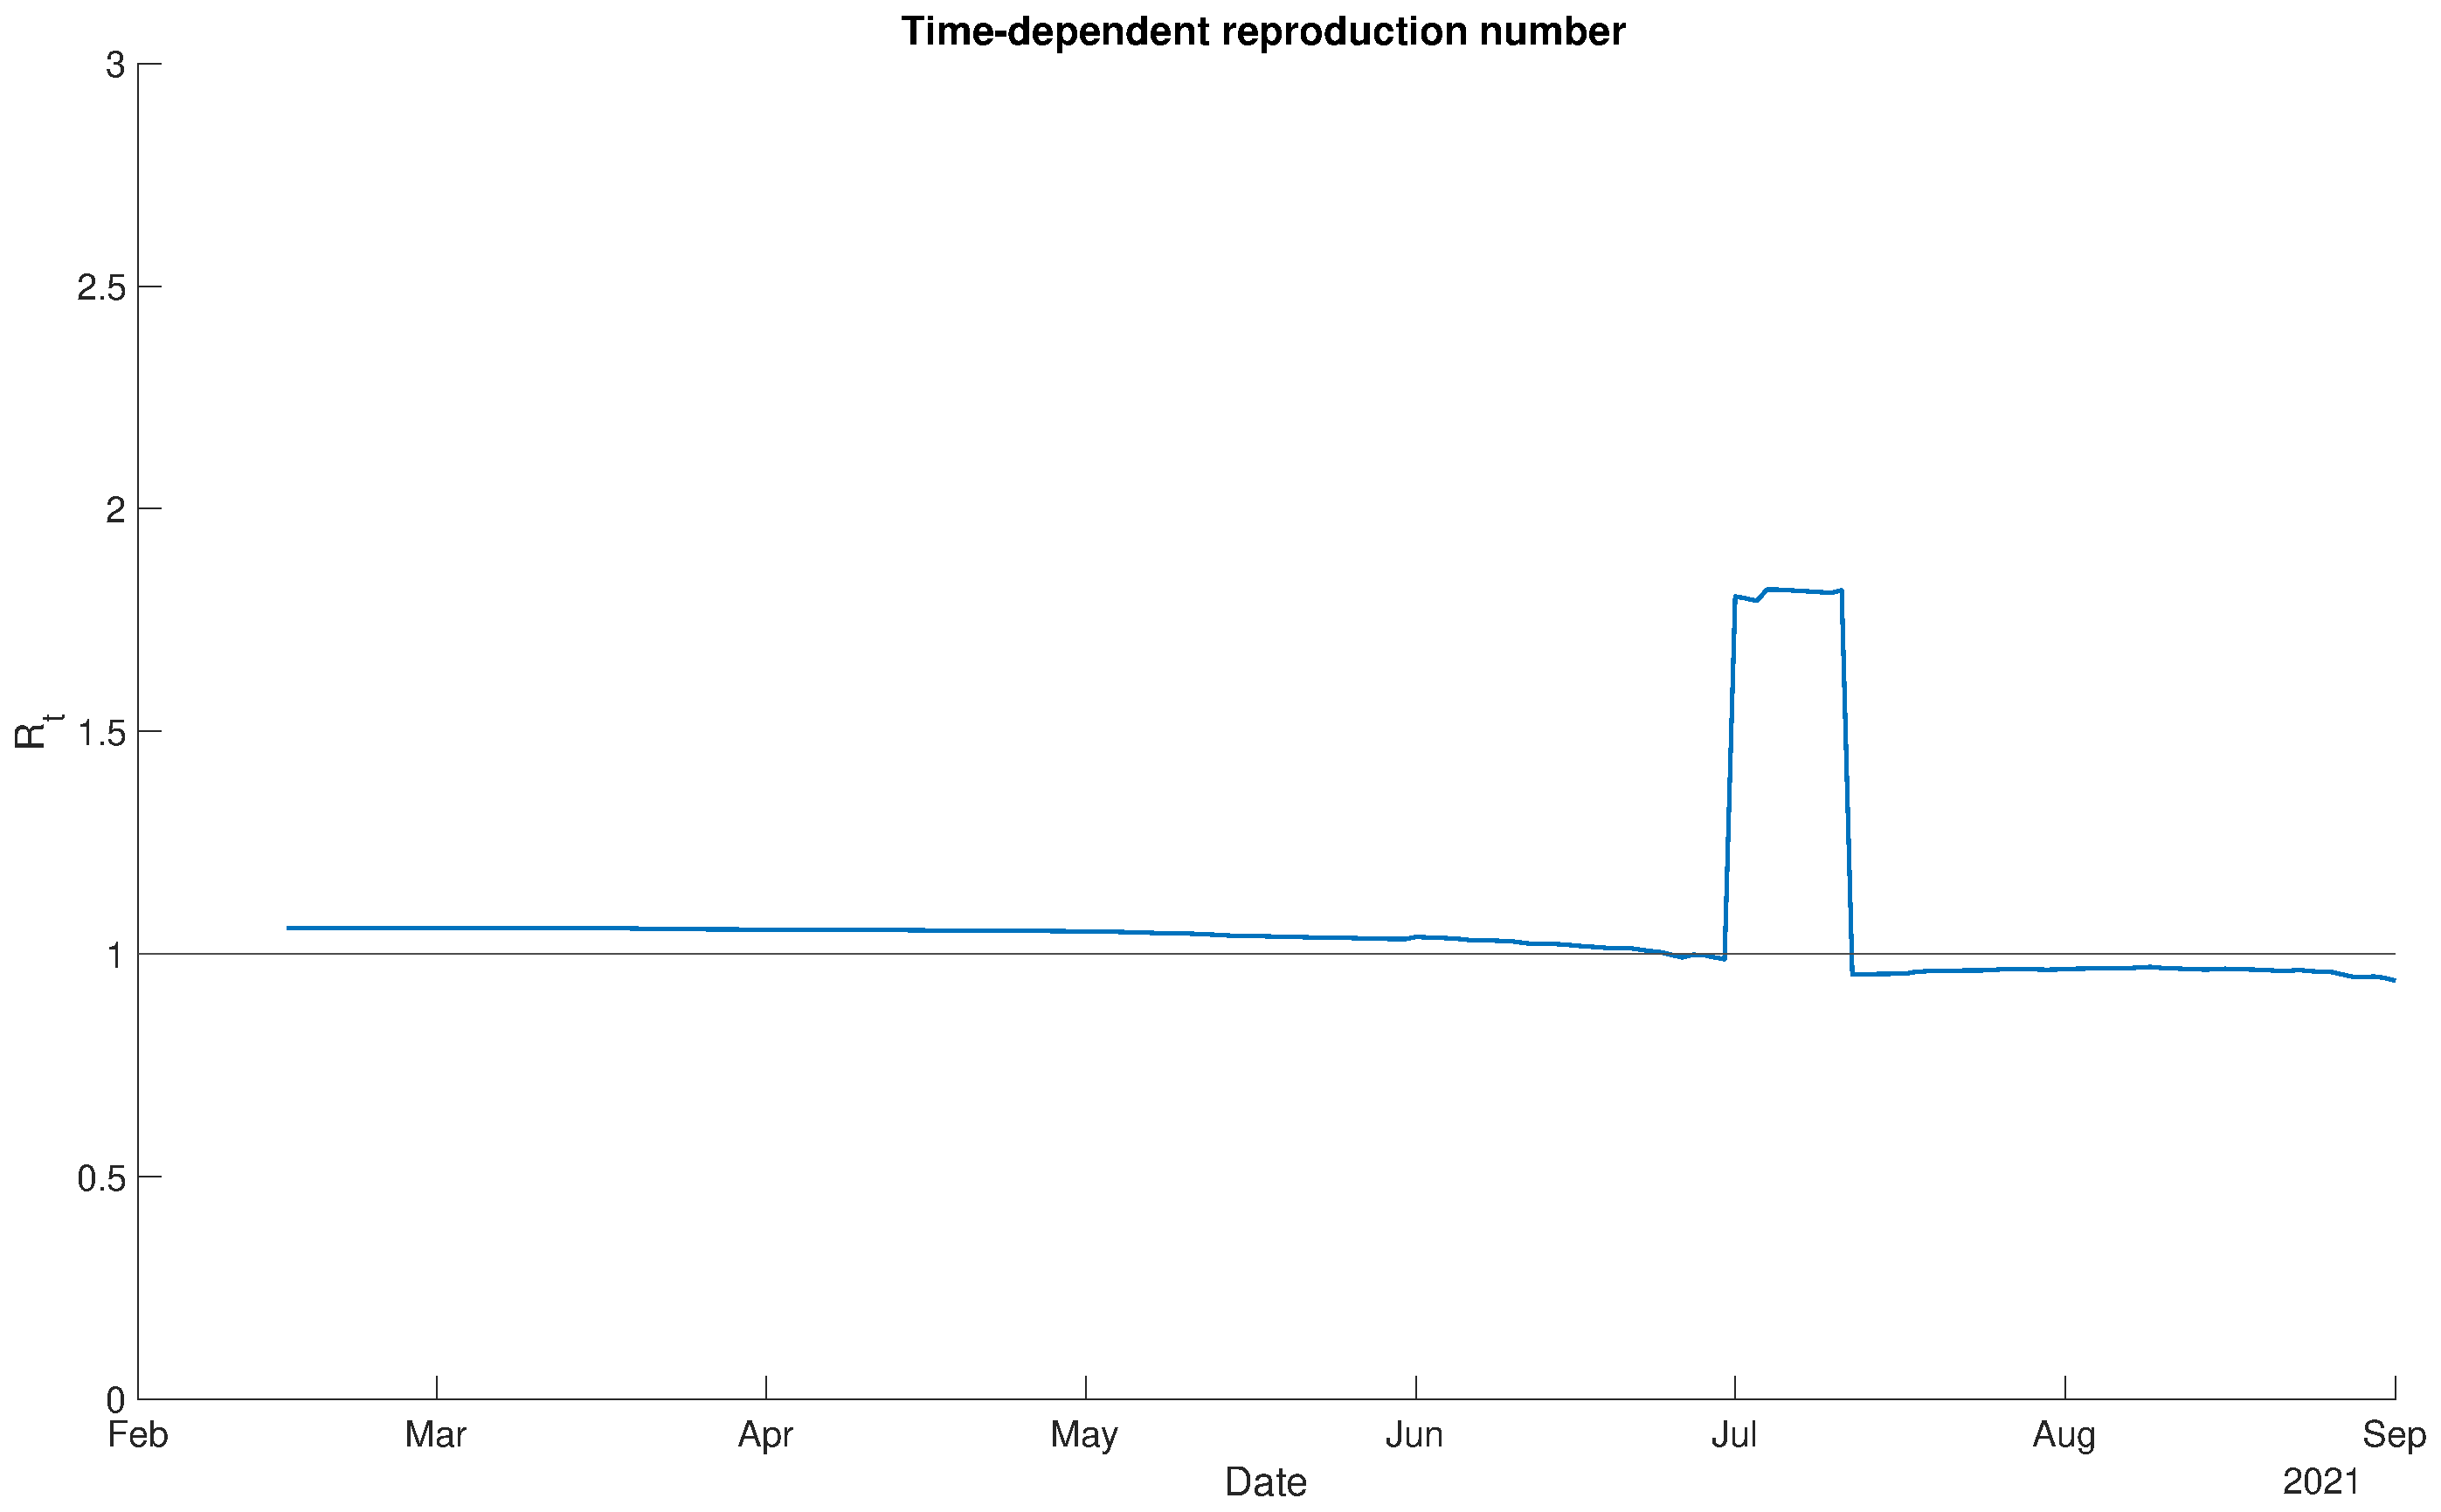
\includegraphics[width=10cm]{../results/estimate_sd_1st_1_2nd_4/rep_num.eps}
	    	\caption{The estimated reproduction number from 2021/02/15 to 2021/09/01.}
	    \end{figure}
	\end{frame}

	\begin{frame}\frametitle{Experiment 5: 1st stage = $\beta \times 1.4161$, 2st stage = $\beta \times 1.4161 \times 0.699 \times 0.35$}
	    \begin{table}
	    	\begin{tabular}{crr}
	    		\toprule
	    		\textbf{Parameter} & \textbf{Initial} & \textbf{Estimate} \\
	    		\midrule
	    		$\delta$ & 1.0000e+00 & 3.4985e+00 \\
Cost & 1.0711e+05 & 1.9969e+04 \\
Time & 0.0000e+00 & 3.0754e+01 \\

	    		\bottomrule
	    	\end{tabular}
	    	\caption{Parameter estimates obtained by maximum likelihood estimation.}
	    \end{table}
	\end{frame}

	\begin{frame}\frametitle{Experiment 5: 1st stage = $\beta \times 1.4161$, 2st stage = $\beta \times 1.4161 \times 0.699 \times 0.35$}
	    \begin{figure}
	    	\centering
	    	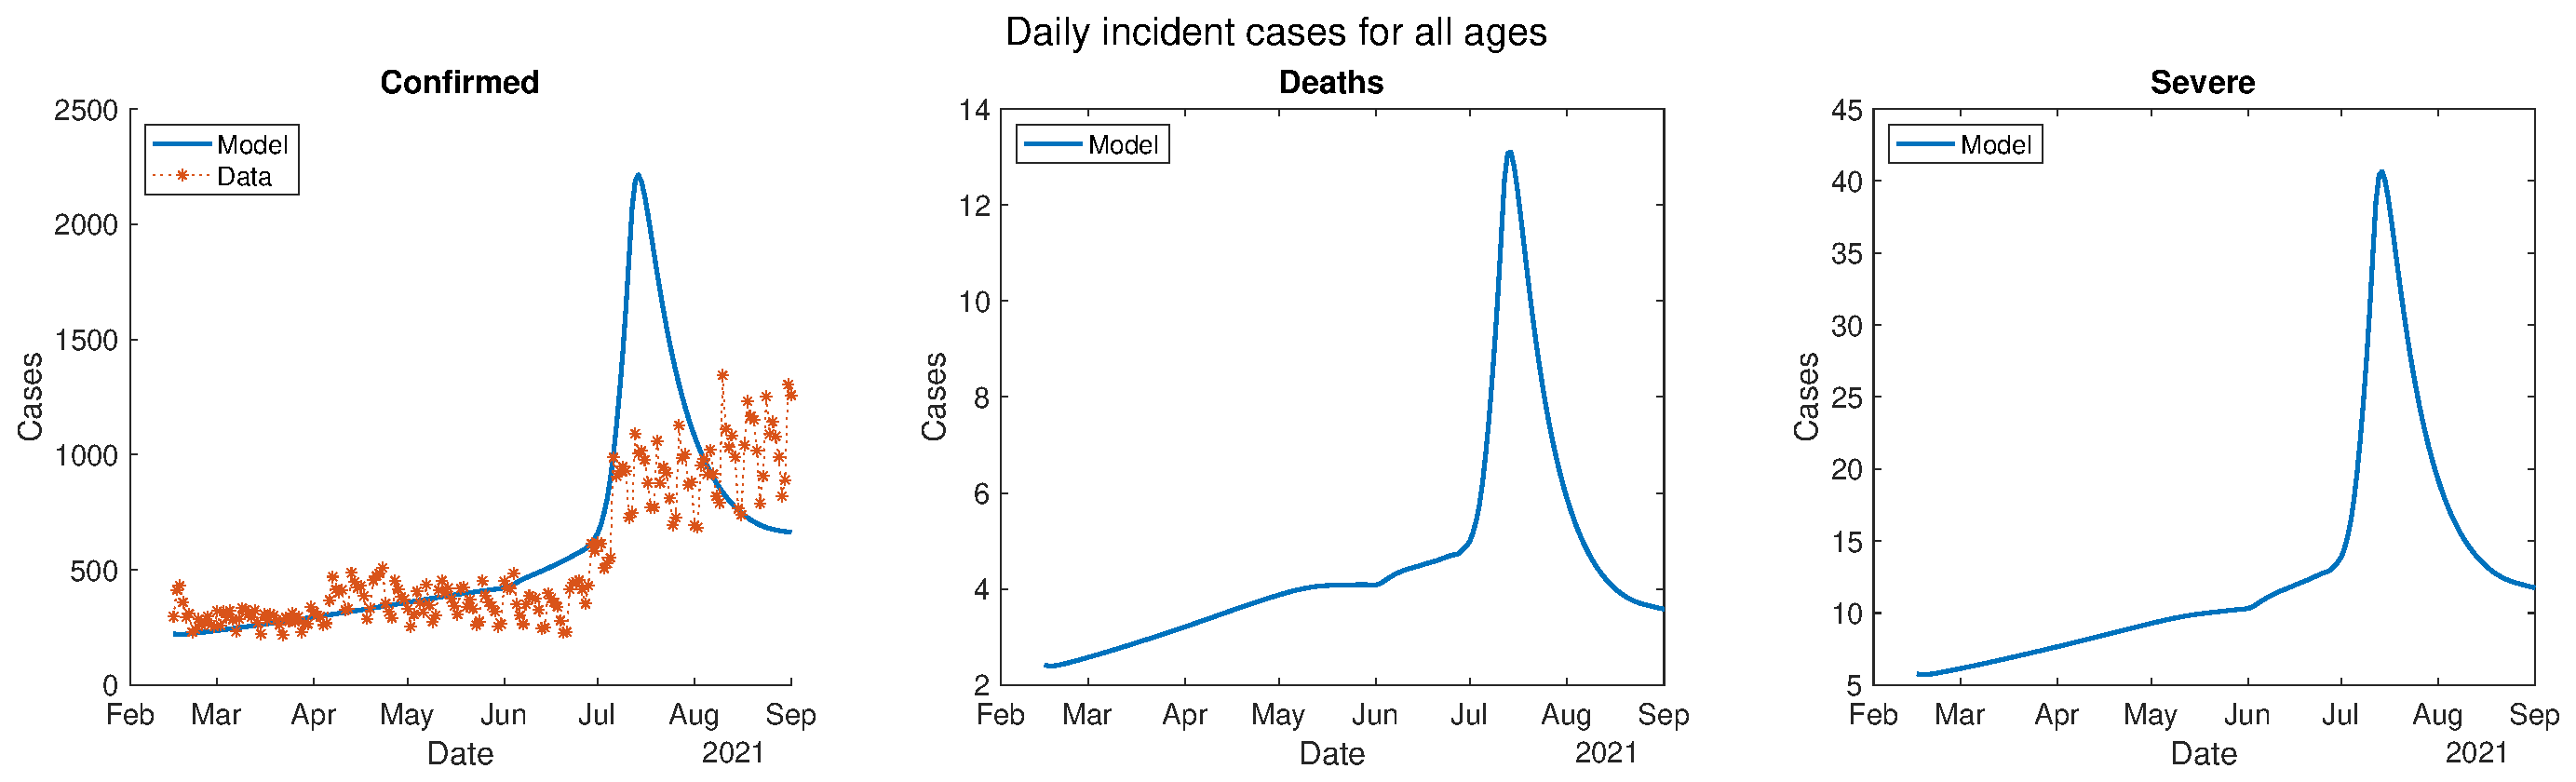
\includegraphics[width=11cm]{../results/estimate_sd_1st_2_2nd_1/daily_all_age.eps}
	    	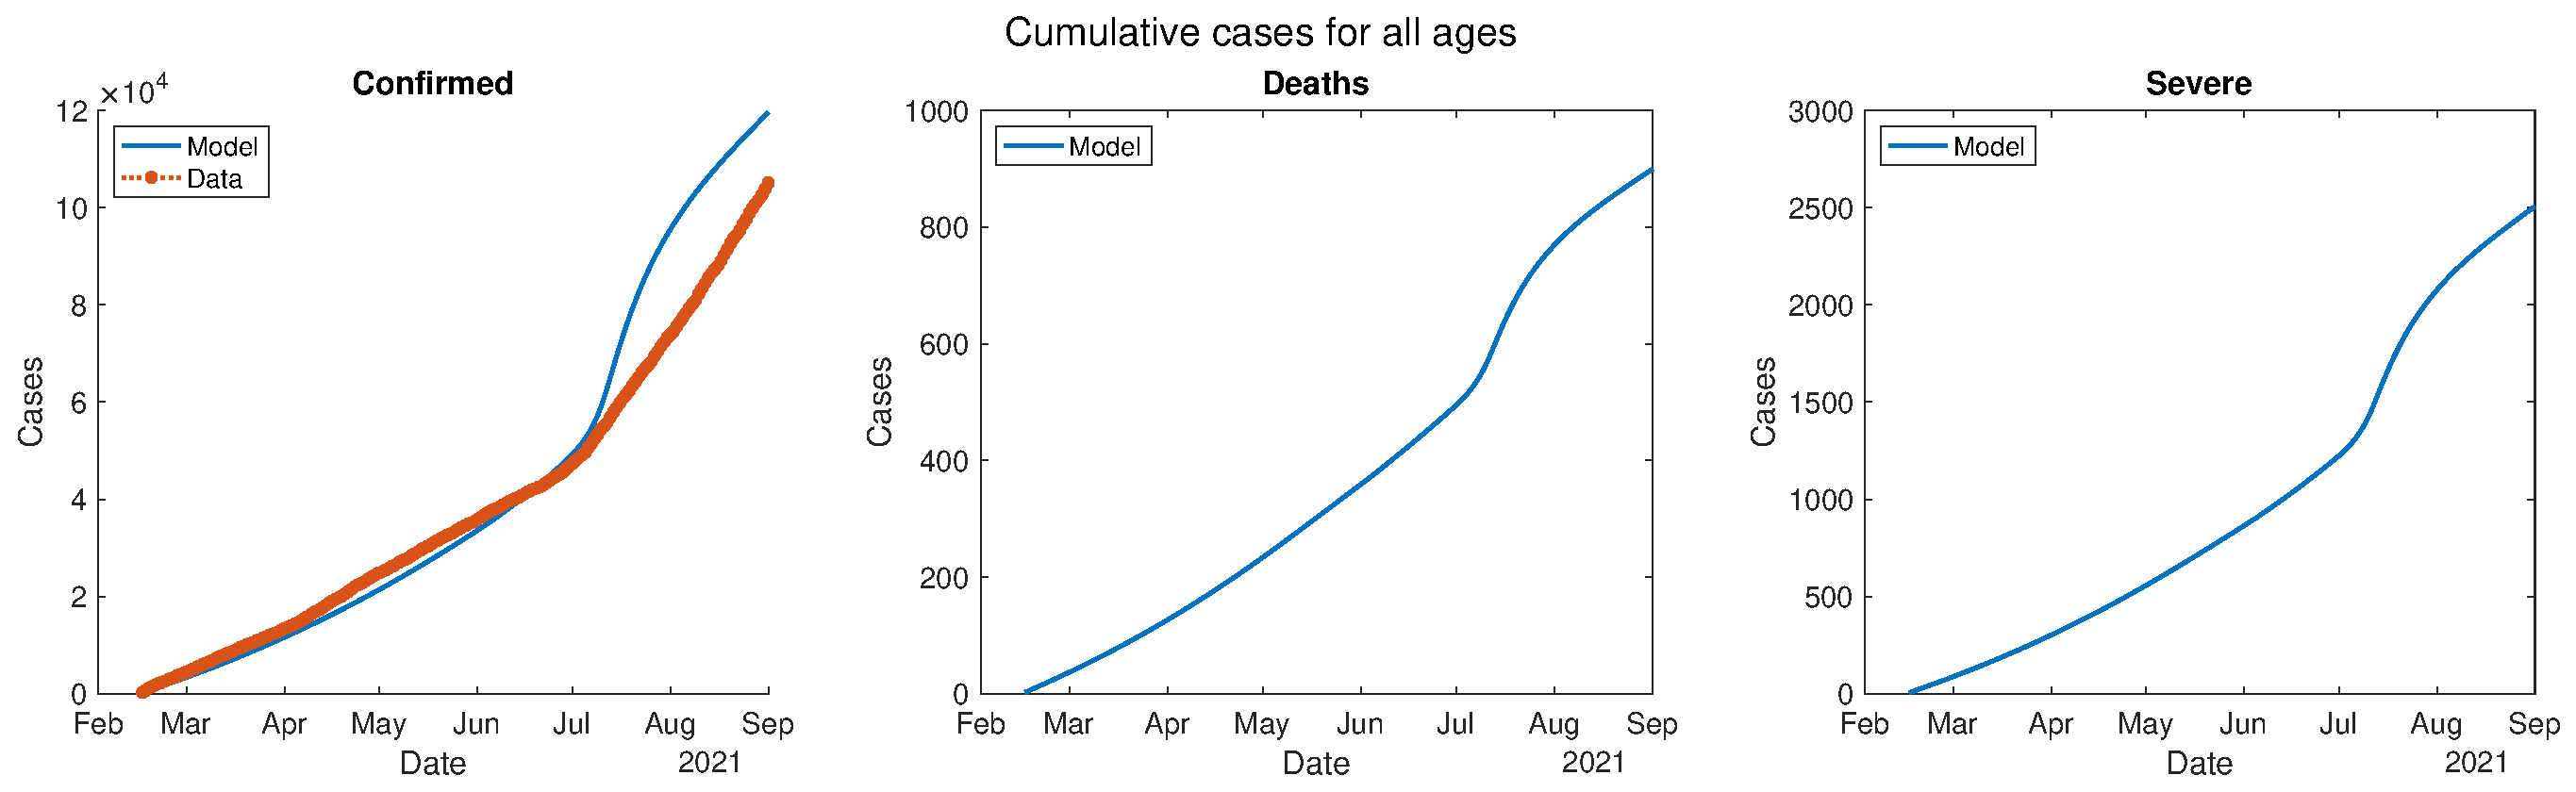
\includegraphics[width=11cm]{../results/estimate_sd_1st_2_2nd_1/cumul_all_age.eps}
	    	\caption{The model prediction and data for daily confirmed cases (top) and cumulative confirmed cases (bottom).}
	    \end{figure}
	\end{frame}

	\begin{frame}\frametitle{Experiment 5: 1st stage = $\beta \times 1.4161$, 2st stage = $\beta \times 1.4161 \times 0.699 \times 0.35$}
	    \begin{figure}
	    	\centering
	    	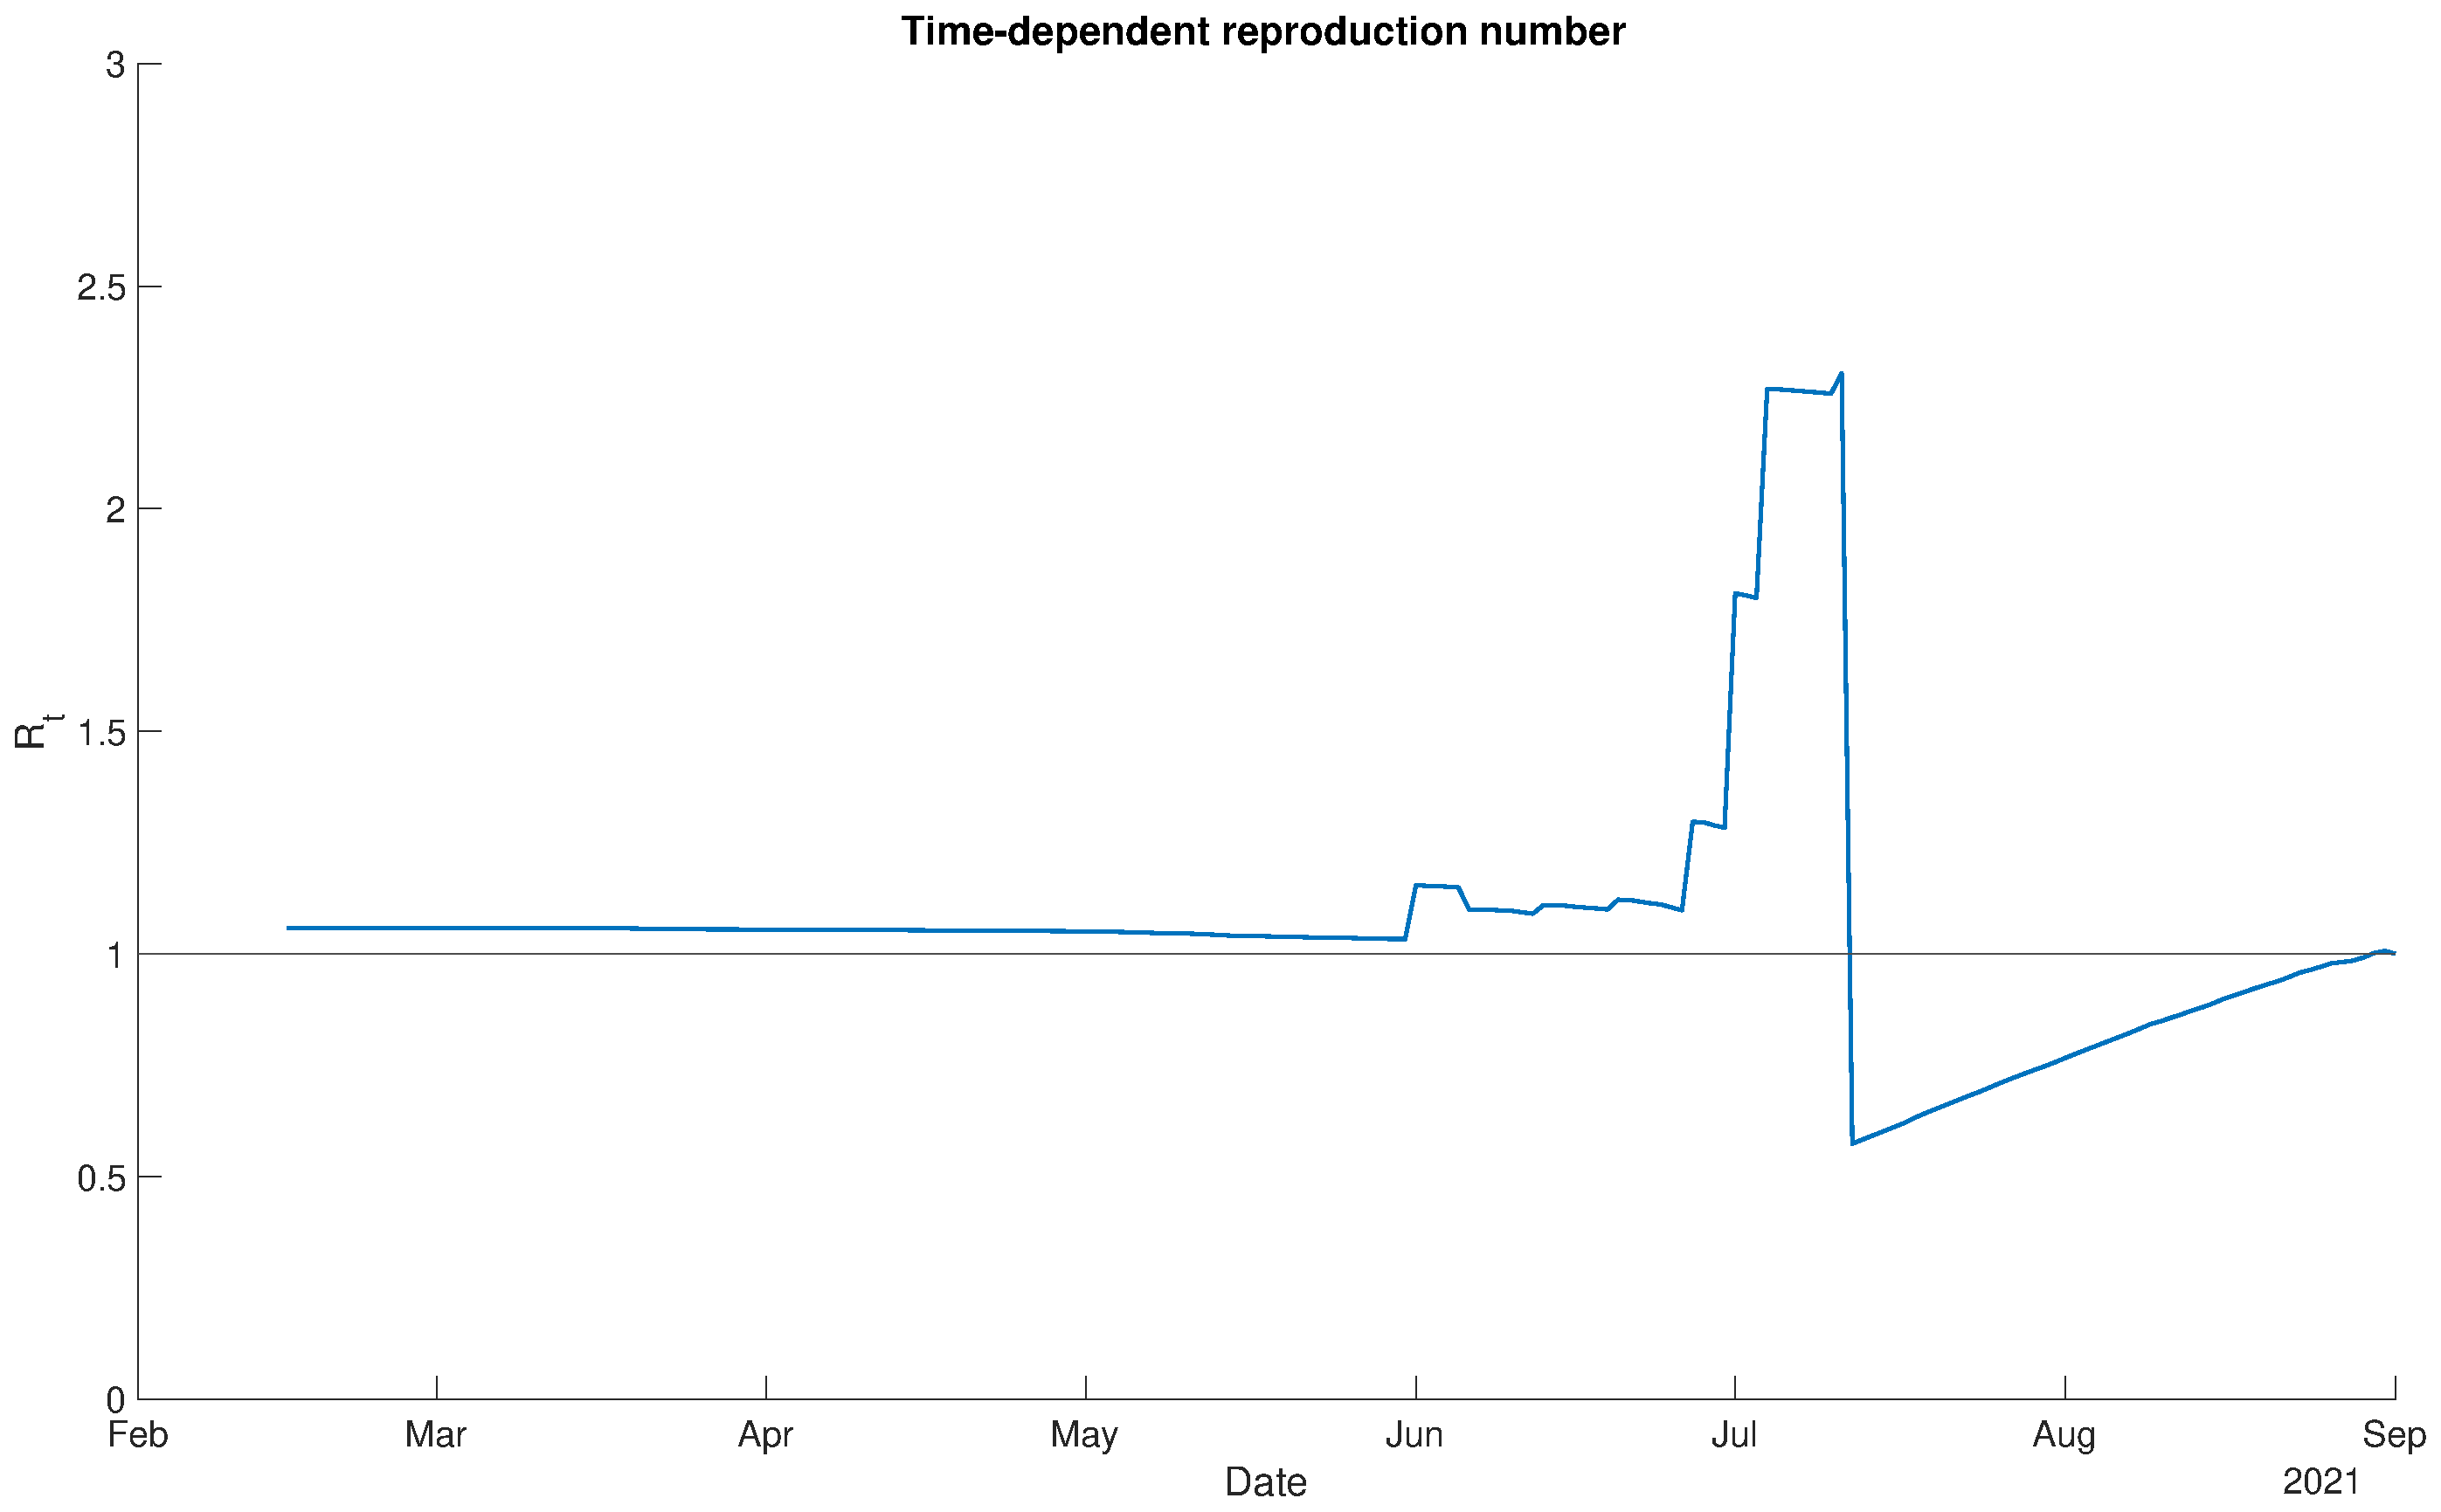
\includegraphics[width=10cm]{../results/estimate_sd_1st_2_2nd_1/rep_num.eps}
	    	\caption{The estimated reproduction number from 2021/02/15 to 2021/09/01.}
	    \end{figure}
	\end{frame}

	\begin{frame}\frametitle{Experiment 6: 1st stage = $\beta \times 1.4161$, 2st stage = $\beta \times 1.4161 \times 0.699$}
	    \begin{table}
	    	\begin{tabular}{crr}
	    		\toprule
	    		\textbf{Parameter} & \textbf{Initial} & \textbf{Estimate} \\
	    		\midrule
	    		$\delta$ & 1.0000e+00 & 1.2532e+00 \\
Cost & 1.9417e+04 & 1.2841e+04 \\
Time & 0.0000e+00 & 2.6832e+01 \\

	    		\bottomrule
	    	\end{tabular}
	    	\caption{Parameter estimates obtained by maximum likelihood estimation.}
	    \end{table}
	\end{frame}

	\begin{frame}\frametitle{Experiment 6: 1st stage = $\beta \times 1.4161$, 2st stage = $\beta \times 1.4161 \times 0.699$}
	    \begin{figure}
	    	\centering
	    	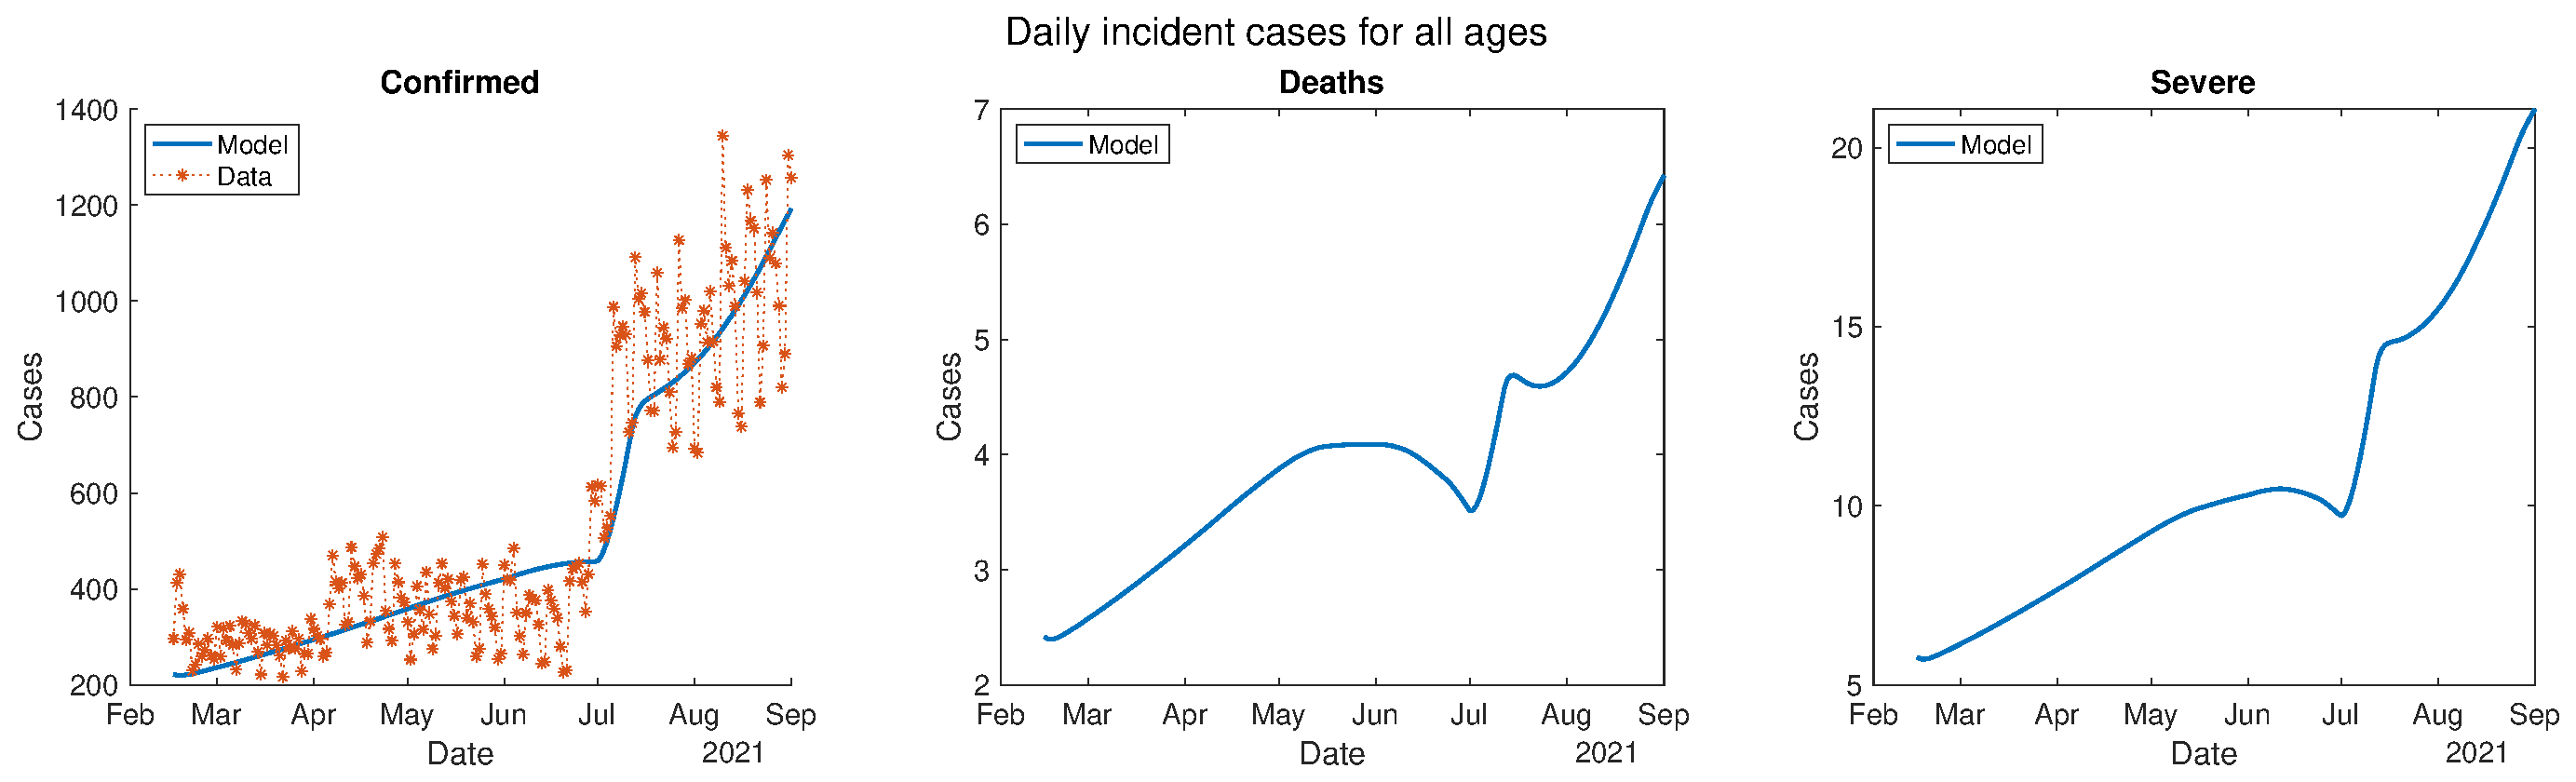
\includegraphics[width=11cm]{../results/estimate_sd_1st_2_2nd_2/daily_all_age.eps}
	    	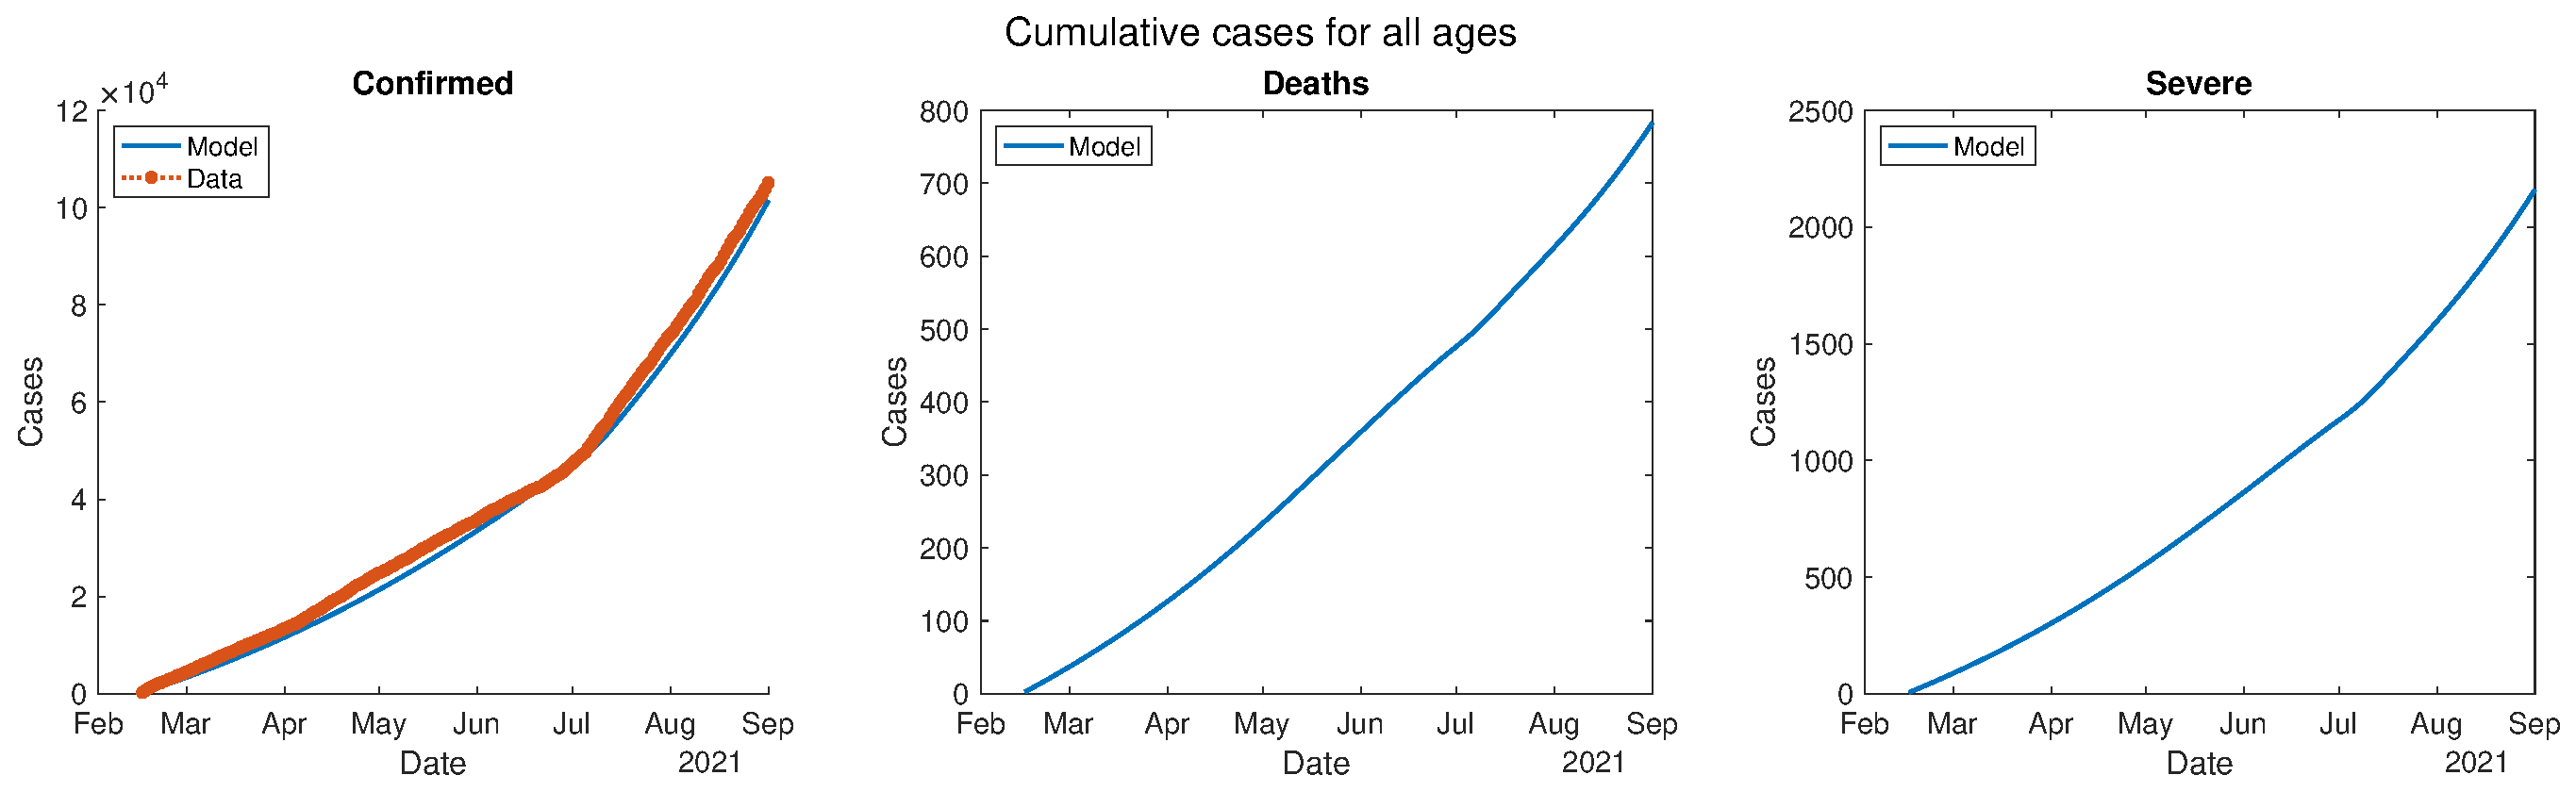
\includegraphics[width=11cm]{../results/estimate_sd_1st_2_2nd_2/cumul_all_age.eps}
	    	\caption{The model prediction and data for daily confirmed cases (top) and cumulative confirmed cases (bottom).}
	    \end{figure}
	\end{frame}

	\begin{frame}\frametitle{Experiment 6: 1st stage = $\beta \times 1.4161$, 2st stage = $\beta \times 1.4161 \times 0.699$}
	    \begin{figure}
	    	\centering
	    	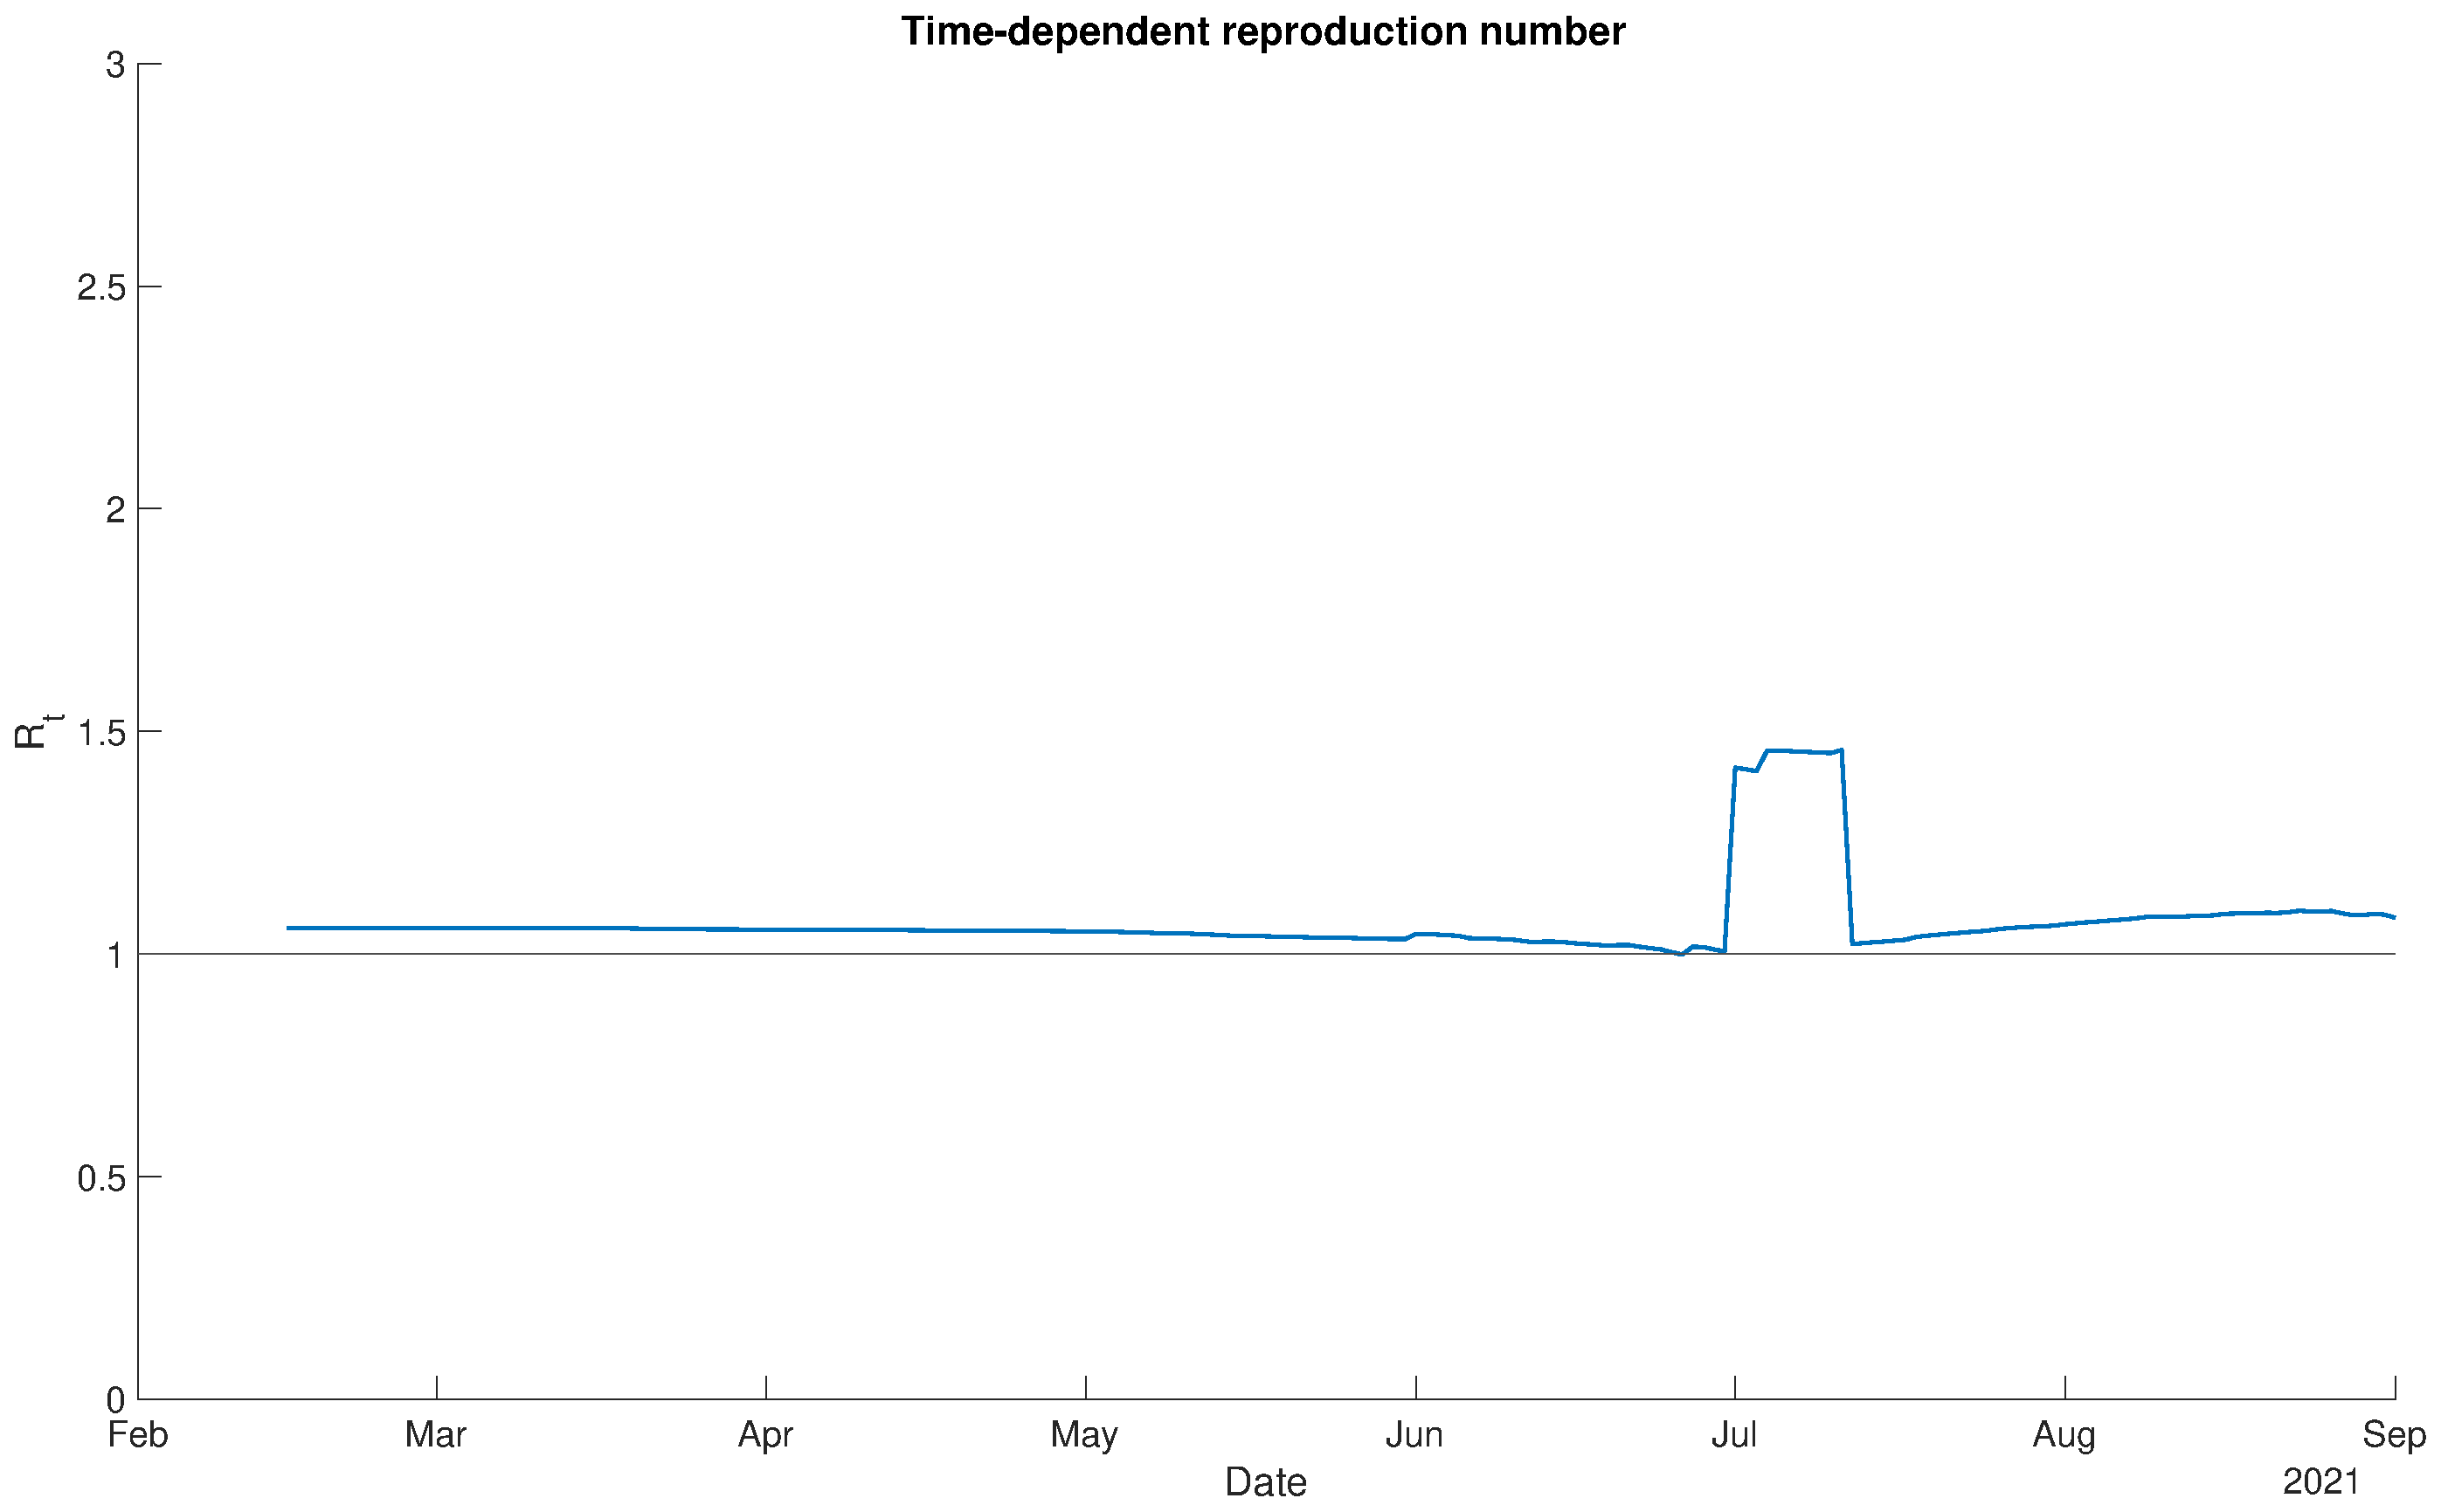
\includegraphics[width=10cm]{../results/estimate_sd_1st_2_2nd_2/rep_num.eps}
	    	\caption{The estimated reproduction number from 2021/02/15 to 2021/09/01.}
	    \end{figure}
	\end{frame}

	\begin{frame}\frametitle{Experiment 7: 1st stage = $\beta \times 1.4161$, 2st stage = $\beta \times 1.4161 \times 0.35$}
	    \begin{table}
	    	\begin{tabular}{crr}
	    		\toprule
	    		\textbf{Parameter} & \textbf{Initial} & \textbf{Estimate} \\
	    		\midrule
	    		$\delta$ & 1.0000e+00 & 2.6626e+00 \\
Cost & 8.3531e+04 & 1.4292e+04 \\
Time & 0.0000e+00 & 3.0413e+01 \\

	    		\bottomrule
	    	\end{tabular}
	    	\caption{Parameter estimates obtained by maximum likelihood estimation.}
	    \end{table}
	\end{frame}

	\begin{frame}\frametitle{Experiment 7: 1st stage = $\beta \times 1.4161$, 2st stage = $\beta \times 1.4161 \times 0.35$}
	    \begin{figure}
	    	\centering
	    	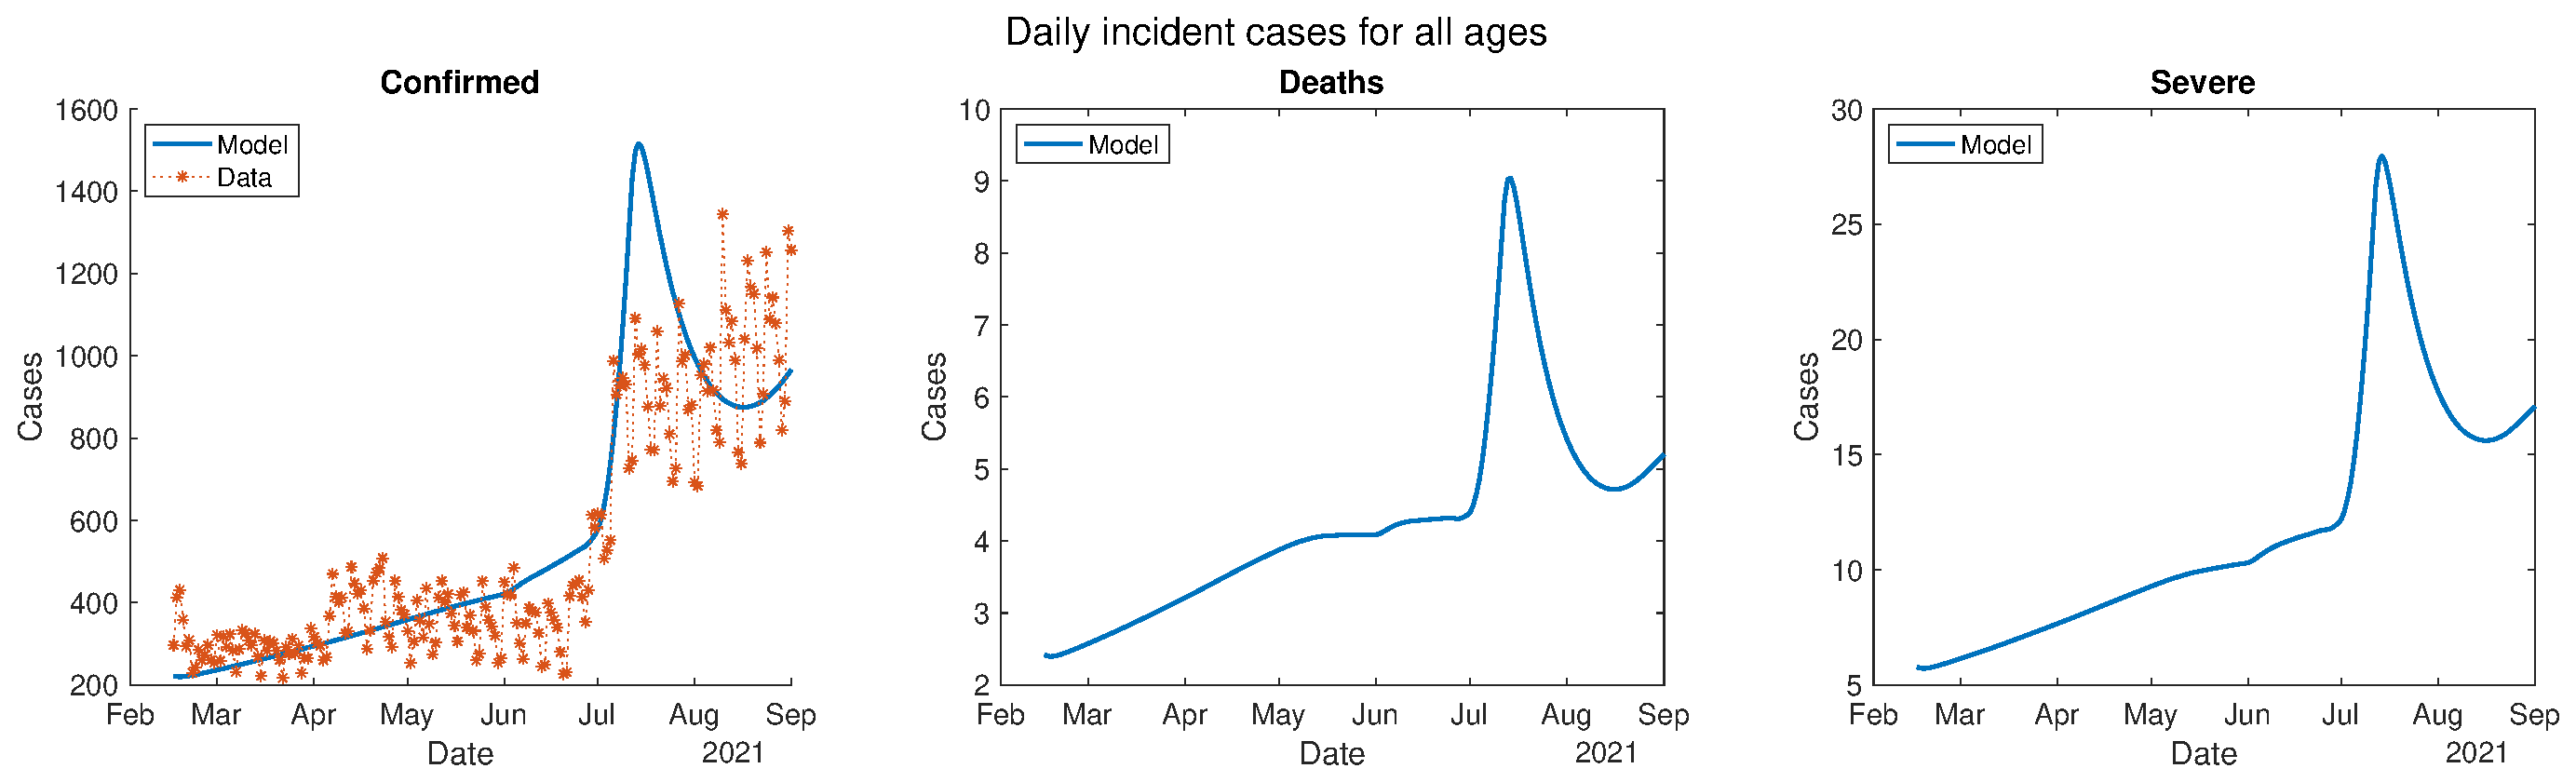
\includegraphics[width=11cm]{../results/estimate_sd_1st_2_2nd_3/daily_all_age.eps}
	    	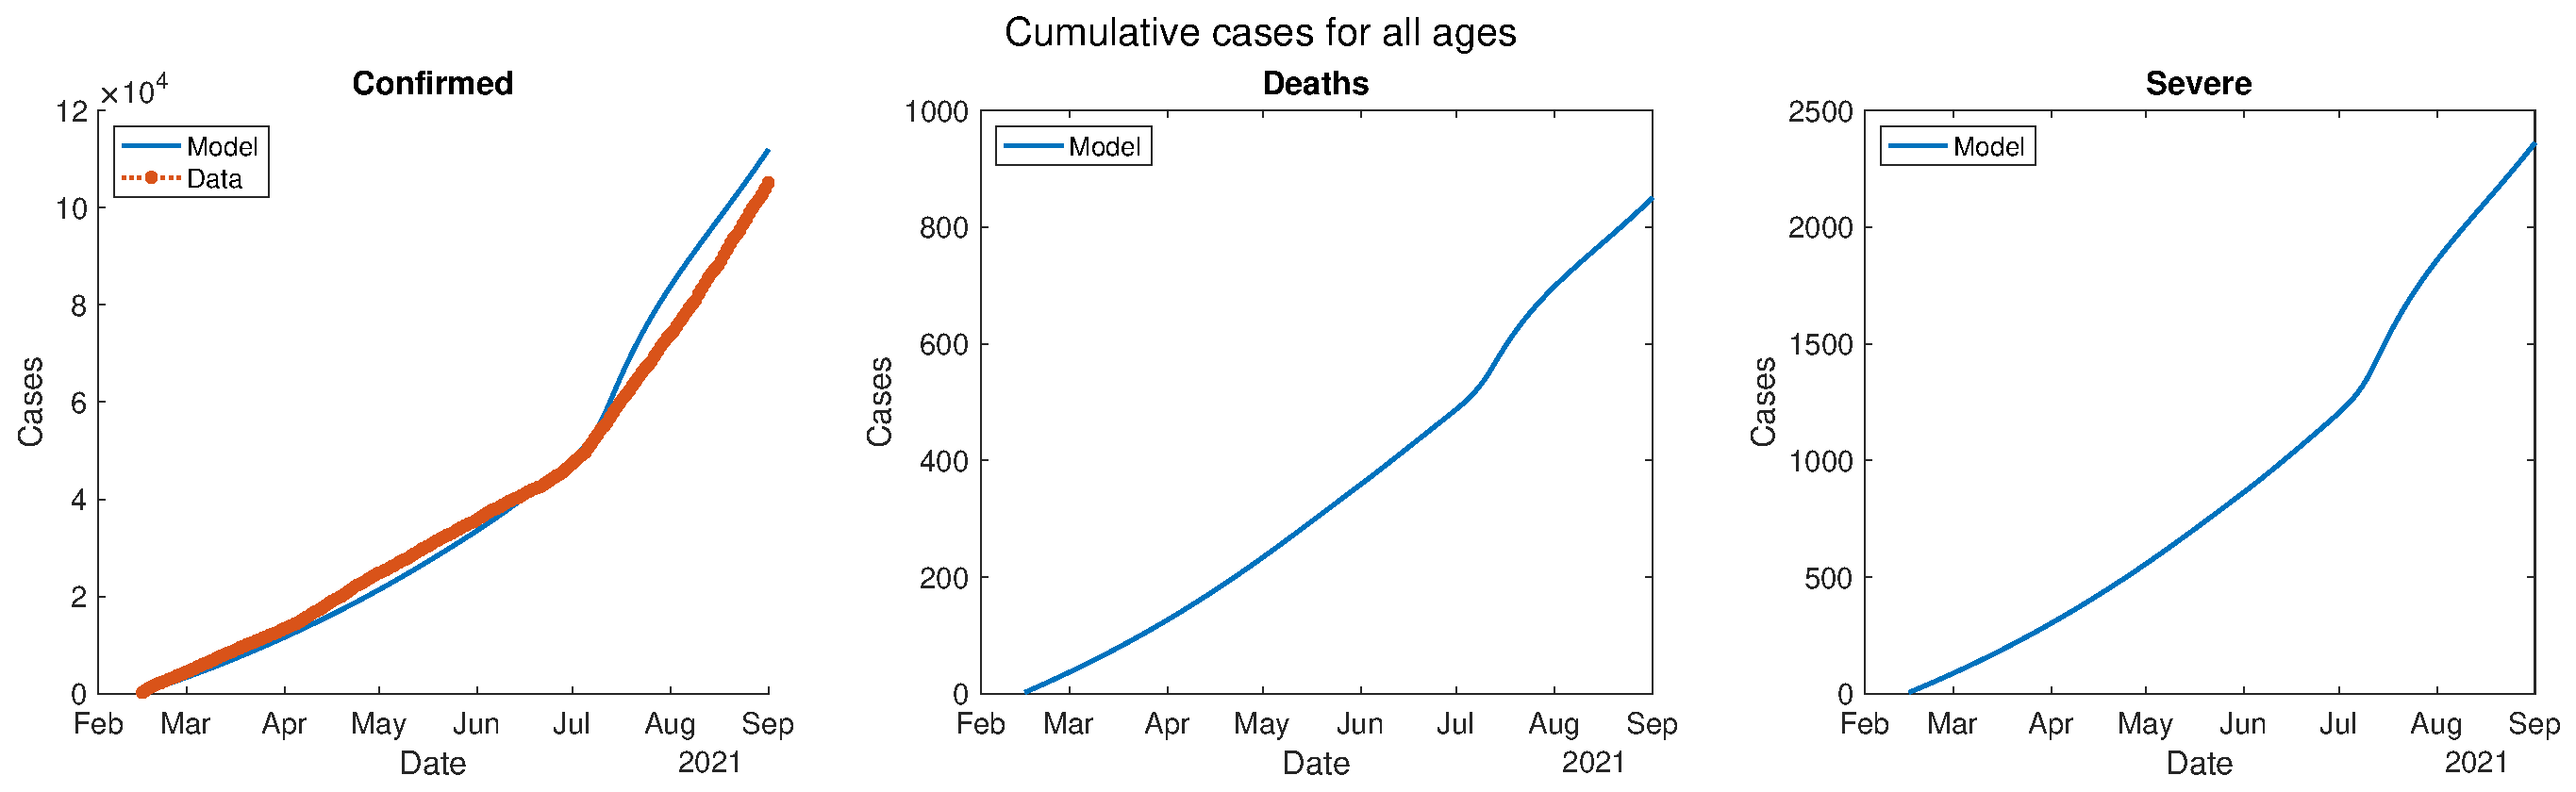
\includegraphics[width=11cm]{../results/estimate_sd_1st_2_2nd_3/cumul_all_age.eps}
	    	\caption{The model prediction and data for daily confirmed cases (top) and cumulative confirmed cases (bottom).}
	    \end{figure}
	\end{frame}

	\begin{frame}\frametitle{Experiment 7: 1st stage = $\beta \times 1.4161$, 2st stage = $\beta \times 1.4161 \times 0.35$}
	    \begin{figure}
	    	\centering
	    	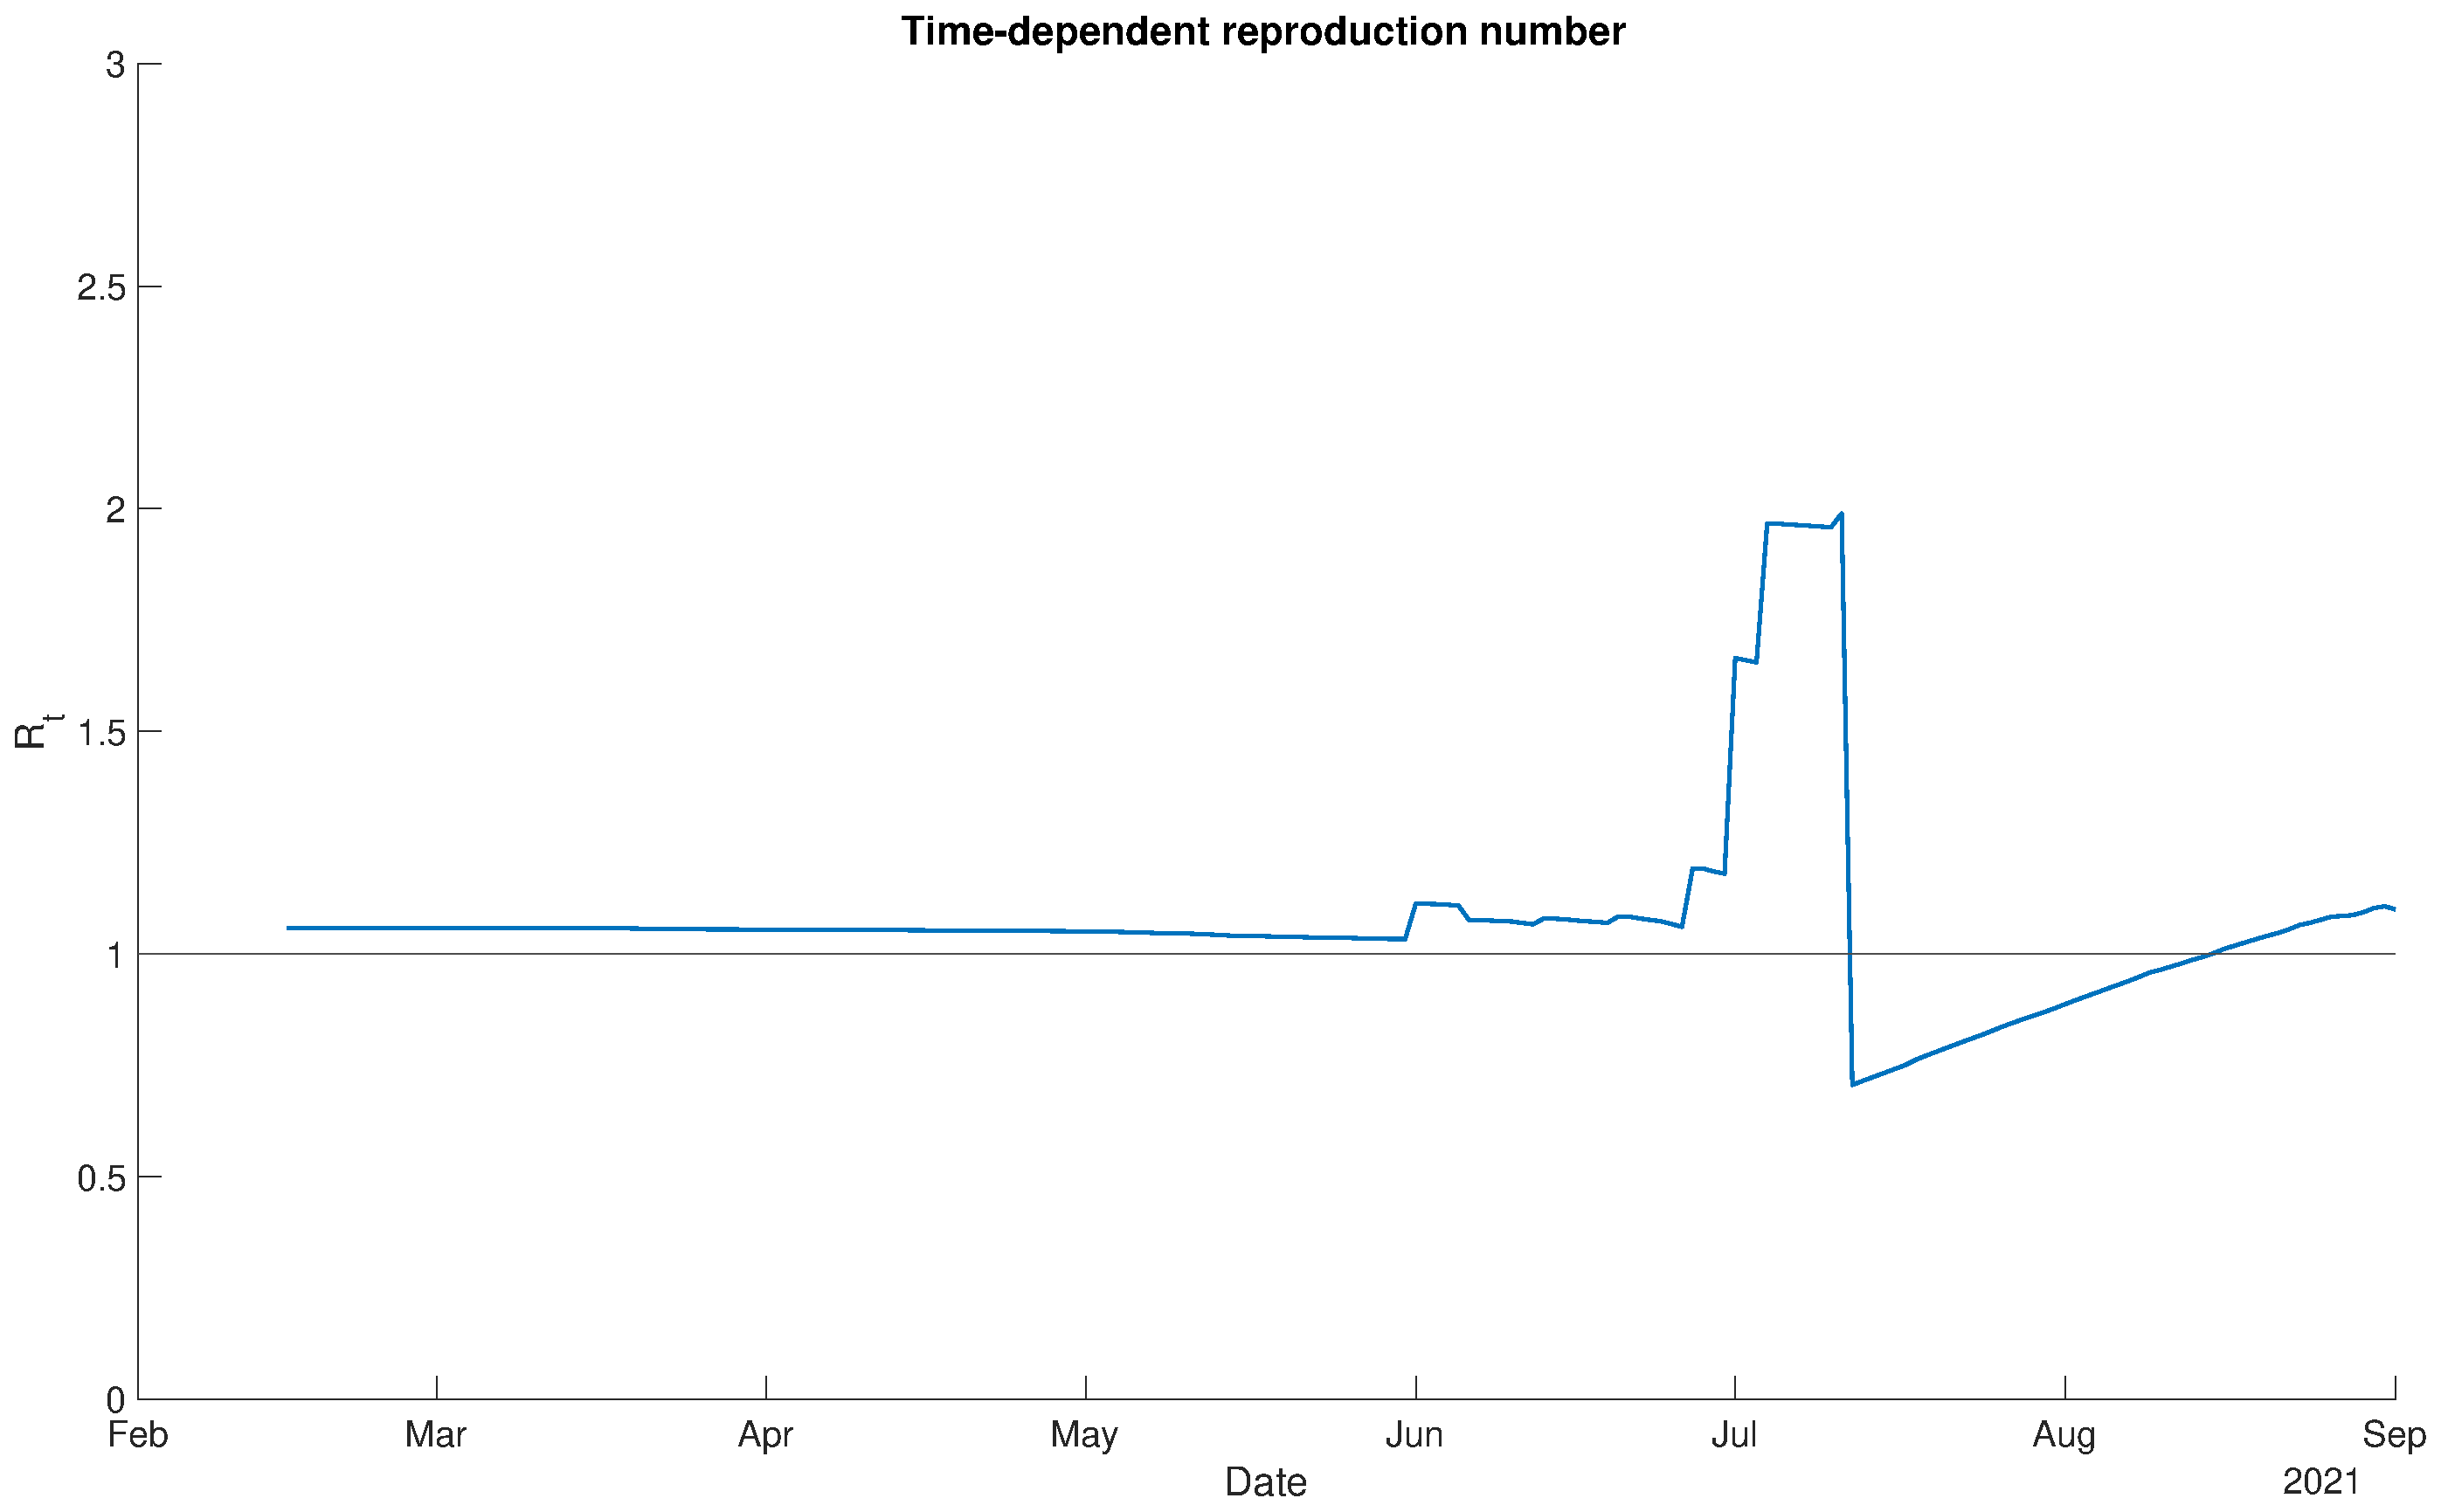
\includegraphics[width=10cm]{../results/estimate_sd_1st_2_2nd_3/rep_num.eps}
	    	\caption{The estimated reproduction number from 2021/02/15 to 2021/09/01.}
	    \end{figure}
	\end{frame}

	\begin{frame}\frametitle{Experiment 8: 1st stage = $\beta \times 1.4161$, 2st stage = $\beta \times 1.4161 \times 0.5245$}
	    \begin{table}
	    	\begin{tabular}{crr}
	    		\toprule
	    		\textbf{Parameter} & \textbf{Initial} & \textbf{Estimate} \\
	    		\midrule
	    		$\delta$ & 1.0000e+00 & 1.7865e+00 \\
Cost & 4.5783e+04 & 1.2556e+04 \\
Time & 0.0000e+00 & 2.8626e+01 \\

	    		\bottomrule
	    	\end{tabular}
	    	\caption{Parameter estimates obtained by maximum likelihood estimation.}
	    \end{table}
	\end{frame}

	\begin{frame}\frametitle{Experiment 8: 1st stage = $\beta \times 1.4161$, 2st stage = $\beta \times 1.4161 \times 0.5245$}
	    \begin{figure}
	    	\centering
	    	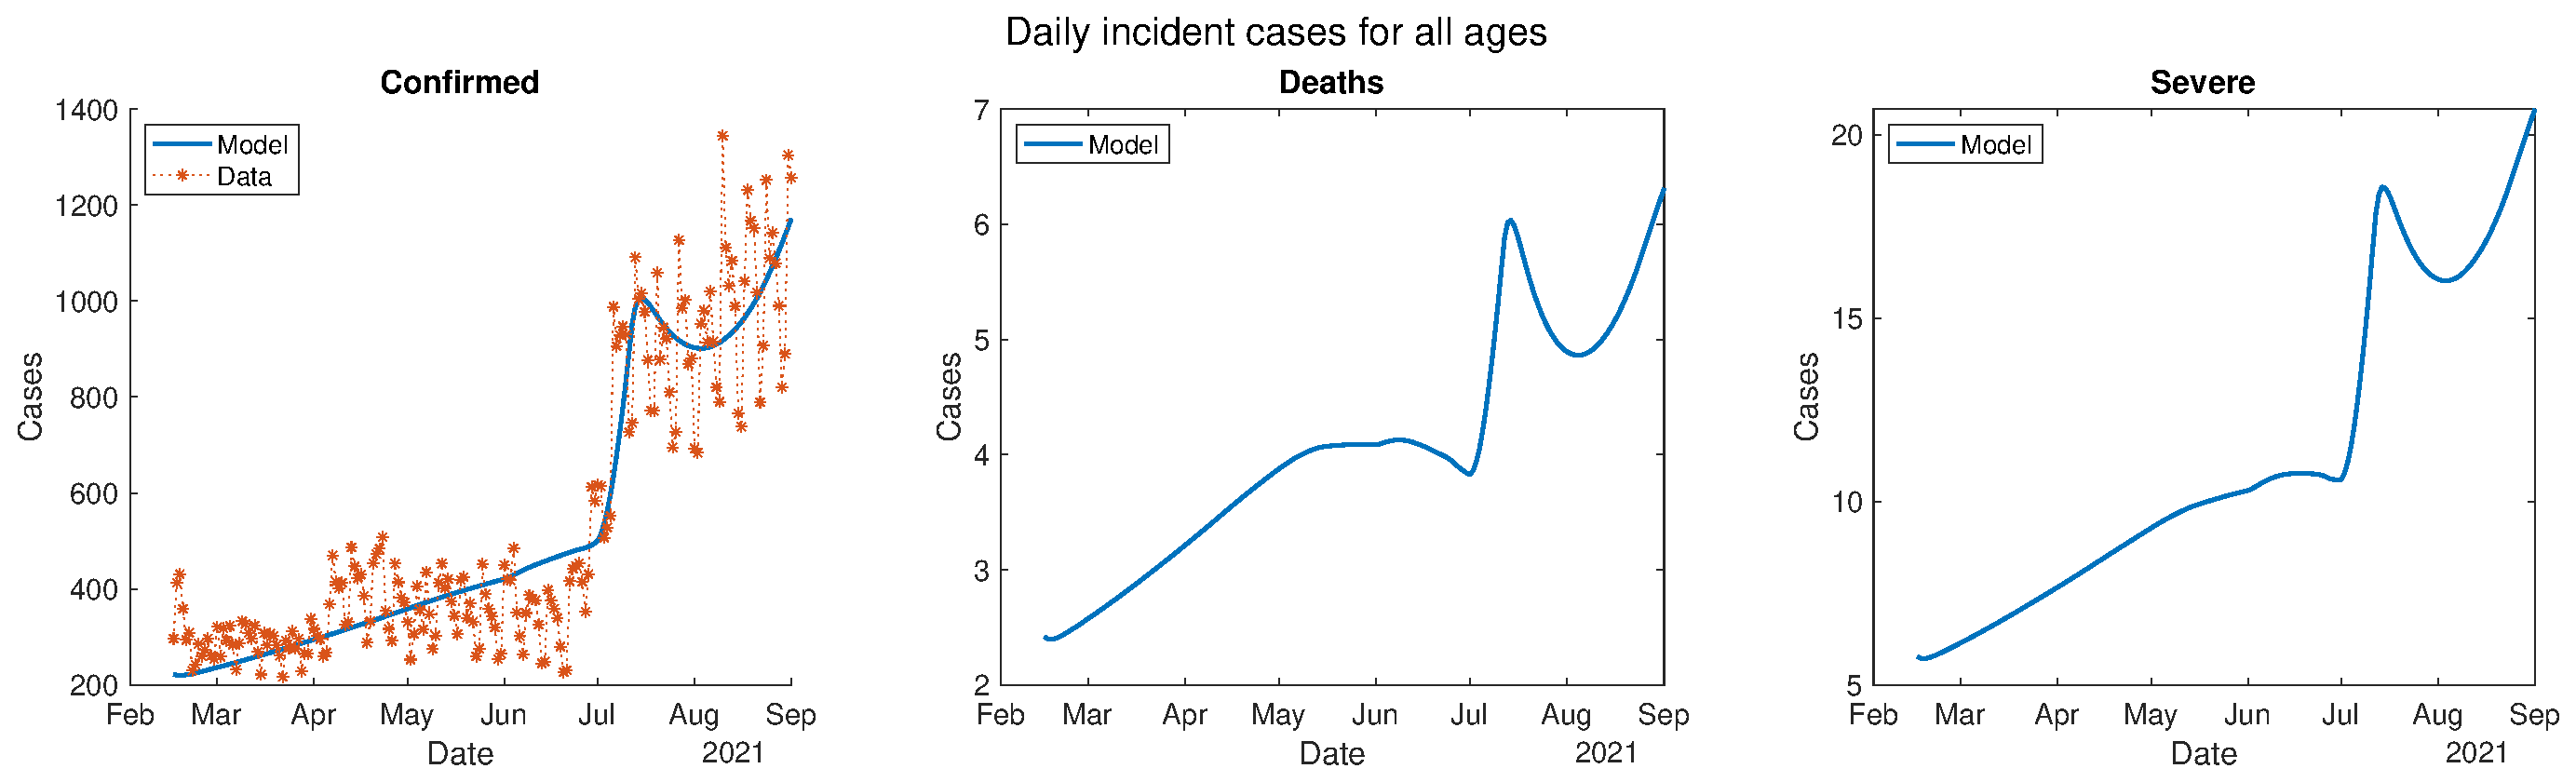
\includegraphics[width=11cm]{../results/estimate_sd_1st_2_2nd_4/daily_all_age.eps}
	    	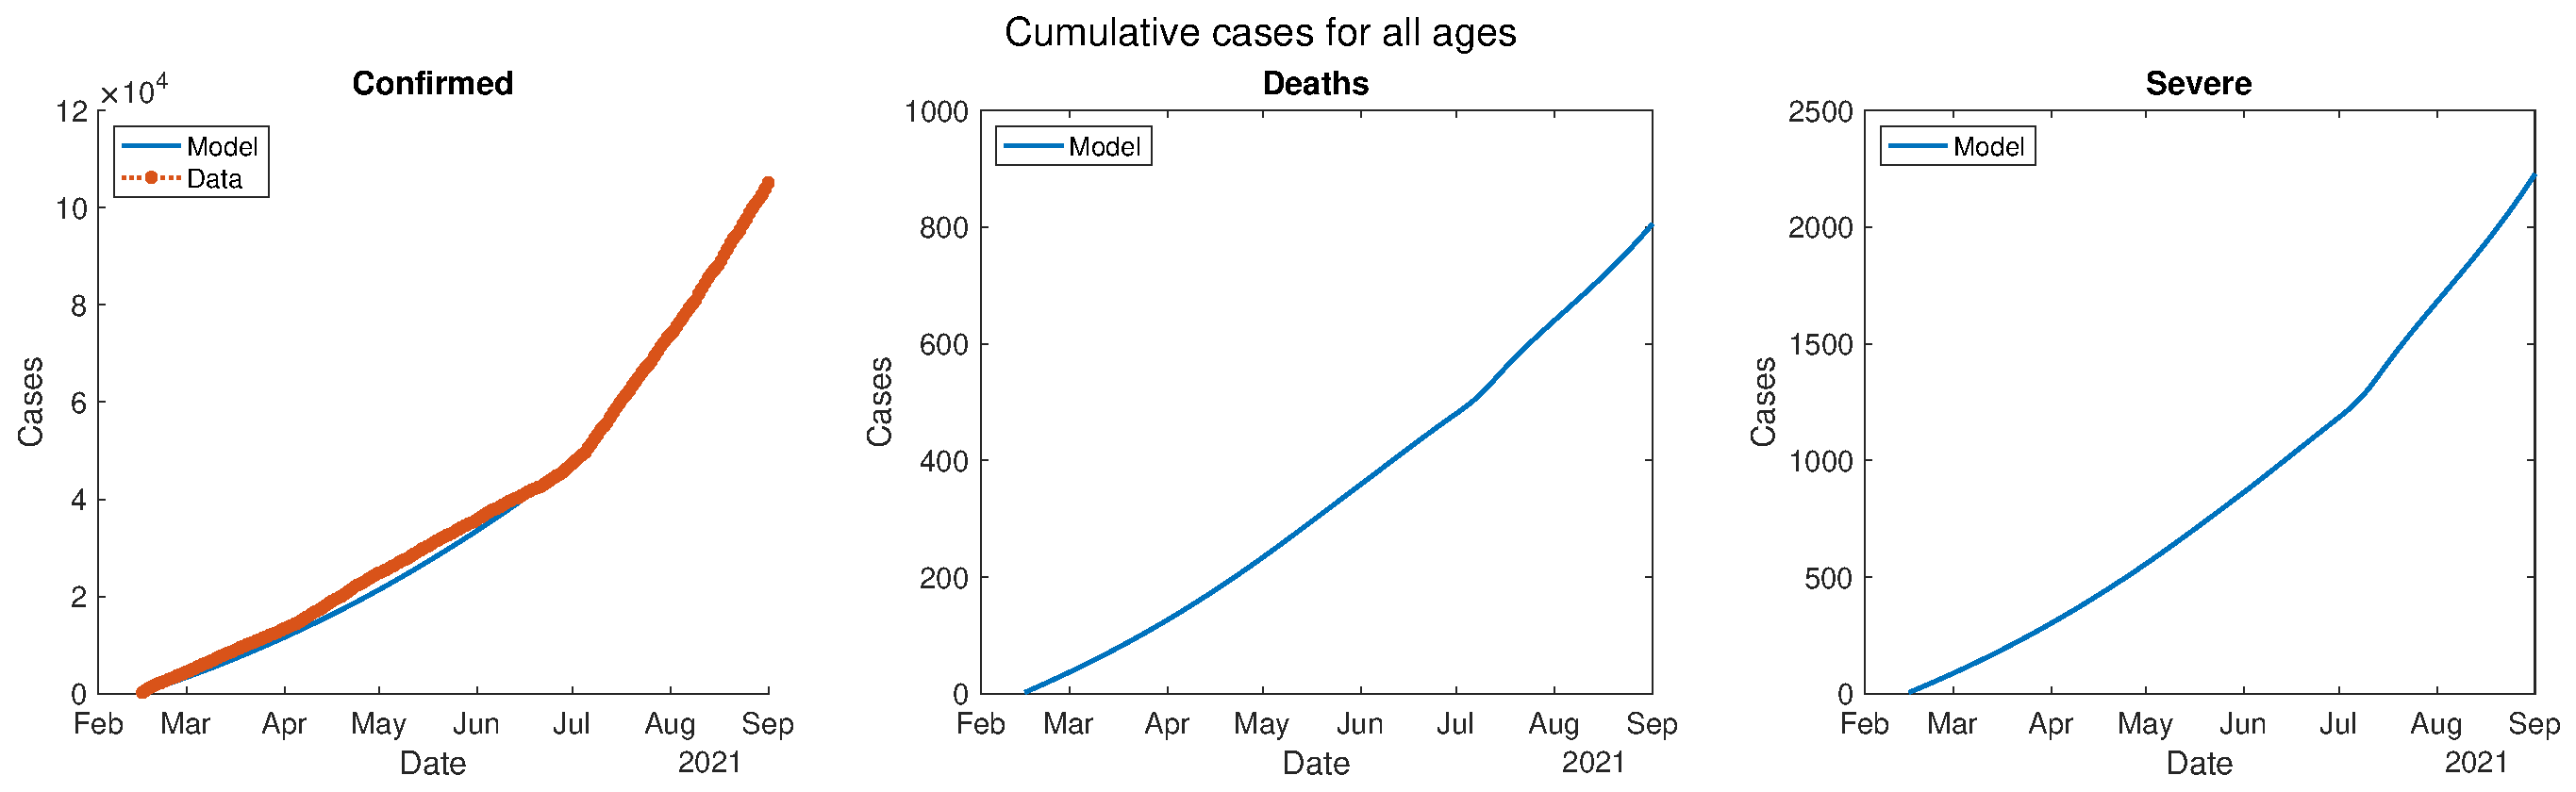
\includegraphics[width=11cm]{../results/estimate_sd_1st_2_2nd_4/cumul_all_age.eps}
	    	\caption{The model prediction and data for daily confirmed cases (top) and cumulative confirmed cases (bottom).}
	    \end{figure}
	\end{frame}

	\begin{frame}\frametitle{Experiment 8: 1st stage = $\beta \times 1.4161$, 2st stage = $\beta \times 1.4161 \times 0.5245$}
	    \begin{figure}
	    	\centering
	    	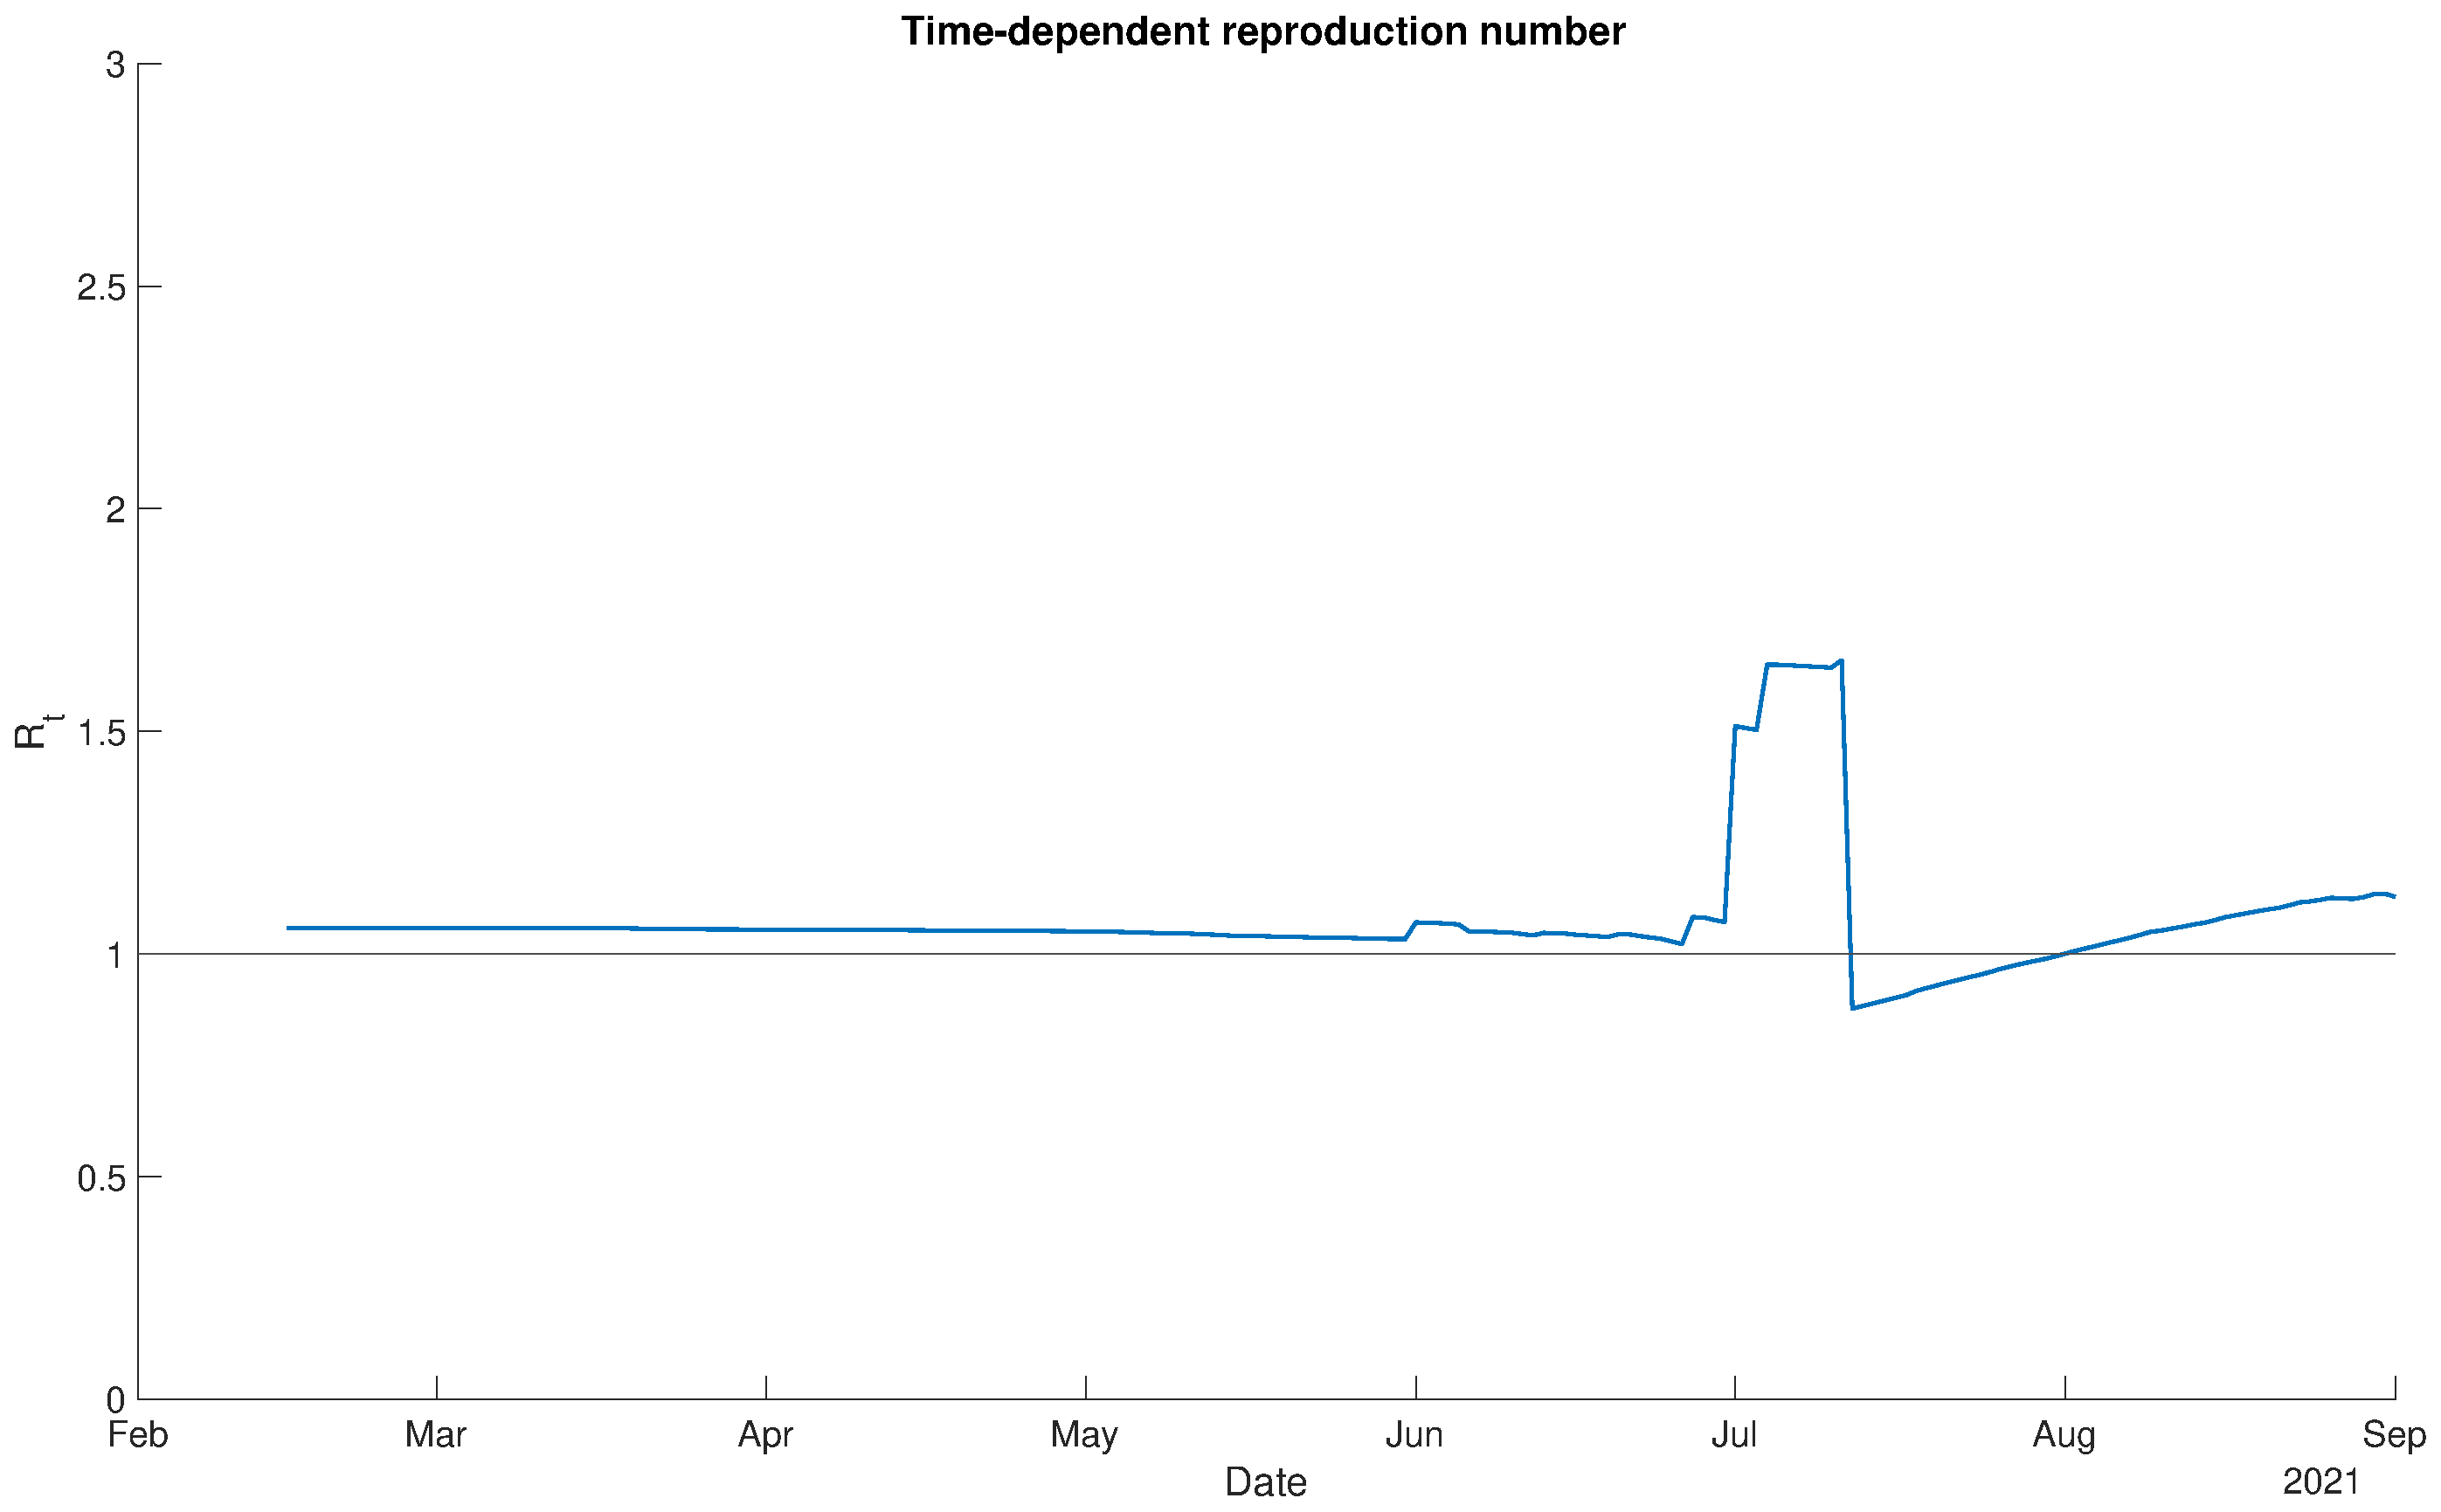
\includegraphics[width=10cm]{../results/estimate_sd_1st_2_2nd_4/rep_num.eps}
	    	\caption{The estimated reproduction number from 2021/02/15 to 2021/09/01.}
	    \end{figure}
	\end{frame}

	\begin{frame}\frametitle{Conclusion}
	    \begin{itemize}
	    	\item 1st stage = $\beta \times 1.4161$, 2nd stage = $\beta \times 1.4161 \times 0.5245$가 $\delta$값이나 피팅 면에서 가장 적합.
	    	\item 큰 $\delta$ 값이 나오기 위해서는 social distancing의 효과가 커야 함.
	    	\item Social distancing의 효과가 크면 산 형태의 dynamics가 나올 수 밖에 없음.
	    	\item 결론적으로 social distancing 효과와 $\delta$ 효과가 서로 compensate하는 관계
	    \end{itemize}	
	\end{frame}

\end{document}